\chapter{Nestor4: telemac2d, various types of reference levels }
%
%****************************************************
% - Purpose & Problem description:
%     These first two parts give reader short details about the test case,
%     the physical phenomena involved and specify how the numerical solution will be validated
%
\section{Purpose (Dig\_by\_time, Backfill\_to\_level. Save\_water\_level)}
%
Example for Nestor:\\
different types of reference levels and Nestor coupled with telemac2d\\
\\
Details about:
\begin{itemize}
  \item coupling Nestor with telemac2d
  \item Order of execution in case of multiple actions
  \item dredging and dumping of the previously dredged material (\texttt{Dig\_by\_time})
  \begin{itemize}
     \item whereby the dumping is controlled by
     \begin{itemize}
        \item a period of time (T$_{\rm{start}}$ - T$_{\rm{end}}$)
        \item a user defined dump rate (dz/dt)
     \end{itemize}
     \item dumping below different types of reference levels
  \end{itemize}
  \item saving a water level at a certain time to use it later as reference level (\texttt{Save\_water\_level})
  \item locally raising the bottom to a defined (arbitrary) shape (\texttt{Backfill\_to\_level})
\end{itemize}

% ***********************************
% **   Description of the problem  **
% ***********************************
\newpage
\section{Description of the problem}
This example is a synthetic test case to demonstrate the above-mentioned tasks.
It's a flat rectangle area (z=0\,m) with four quadratic rising grounds (z=1\,m) and four cone-shaped
depressions (deepest point = -5\,m) (fig.\,\ref{geom3D}).
Nestor is coupled directly with telemac2d

\begin{figure} [H]
 \centering
 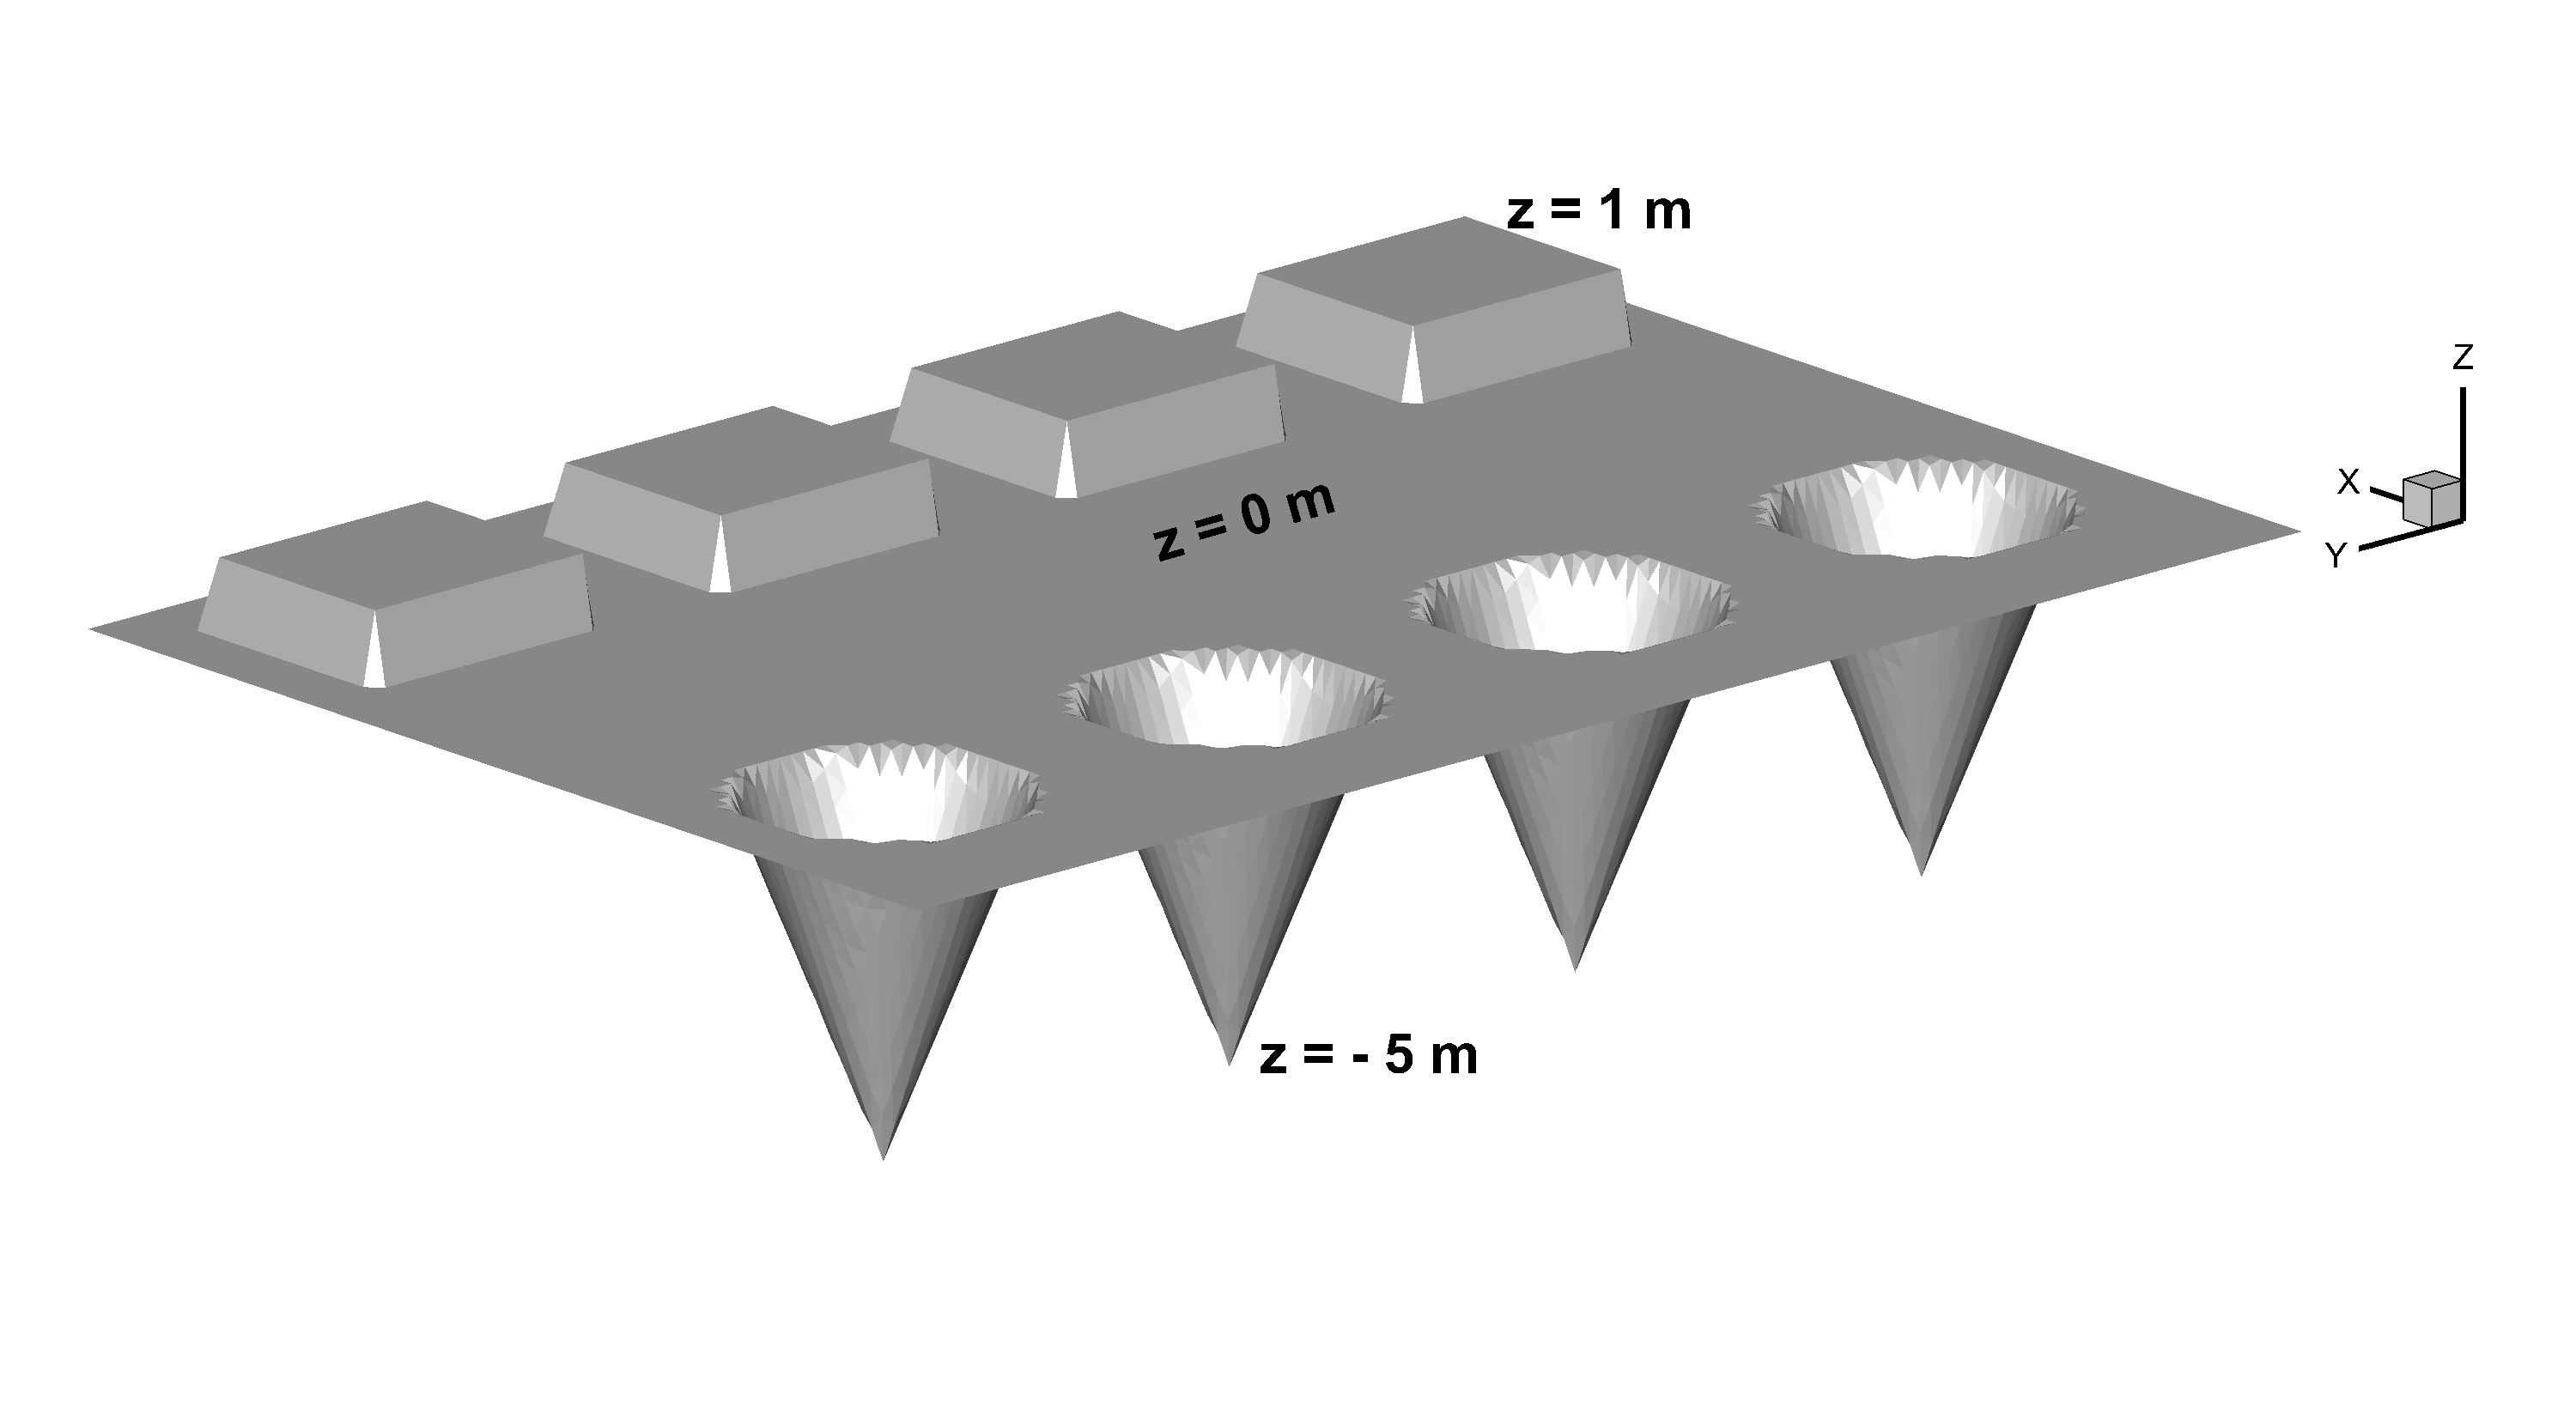
\includegraphics[scale=0.15]{img/Bild_BottomGeometrie_3D.png}
 \caption{Initial bottom geometry (vertical exaggeration 5x)}
 \label{geom3D}
\end{figure}

To run Nestor with telemac2d in the steering file (\texttt{t2d\_nestor4.cas})
settings for the Nestor related keywords are be done as shown below:
\\ \texttt{\small{NESTOR~~~~~~~~~~~~~~~~~~~~~~~~= YES}}
\\ \texttt{\small{NESTOR ACTION FILE~~~~~~~~~~~~= \_DigActions.dat}}
\\ \texttt{\small{NESTOR POLYGON FILE~~~~~~~~~~~= \_DigPolys.dat}}
\\ \texttt{\small{NESTOR SURFACE REFERENCE FILE~= \_DigRefLevel.dat}}
\\ \texttt{\small{ORIGINAL DATE OF TIME~~~~~~~~~= 2000;01;01~~~~/ year,~month,~~day}}
\\ \texttt{\small{ORIGINAL HOUR OF TIME~~~~~~~~~= 0;0;0~~~~~~~~~/ hours,minutes,seconds}} \\
\\
The example shows four dredge actions (\texttt{Dig\_by\_time}) in which the
mounds will be dredged away (more or less) and the dredged material
will be dumped in different ways into the depressions.
Additionally it shows how Nestor can be used to change the bottom to an arbitray shape (\texttt{Backfill\_to\_level}).
The actions are defined in the action file (Nestor steering file) \texttt{~\_DigActions.dat}.
The areas where the dredging and dumping will be done are defined by polygons (fig.\,\ref{geom2D})
which are stored in the file \texttt{\_DigPolys.dat}.\\
In case of \texttt{~DumpPlanar\,=\,TRUE~} a reference level is used for the dumping.
\\
\newpage
\subsubsection{Settings due to performance issues when run the example}
Because the examples are used to run in an automated test suite, same parameter
settings are done to obtain slim output files.
To obtain a result file which matches (by time) the images fig.\,\ref{Act1}, \,\ref{Act3} to\,\ref{Act6}, change the settings in the telemac steering file
as follows and run the example again.
\\ \texttt{\small{GRAPHIC PRINTOUT PERIOD = 3,  LISTING PRINTOUT PERIOD = 1}}

% ***********************************************
% **   order of execution   Nestor Graphic   ****
% ***********************************************
%\newpage
\subsection{Multiple actions and order of execution}\label{ssec:E4OrderExc}
If multiple actions are defined the internal numbering of the actions follows the order of appearance in the action file.\\
\\
\fcolorbox{green}{yellow}{
  \parbox{1.0\linewidth}{Order of execution in case there are multiple actions defined:
  \begin{itemize}
  \item{On the first level, the order of execution depends on the timeline.}
  \item{On the second level, if several actions are active at the same time or start at the same time,
        the numbering of the actions is significant to the order of execution during one time step.}
  \end{itemize}
}}
\textcolor{white}{force a empty line by white lettering}\\ %----- white line-----

% *********  Nestor Graphic  ***********************
During the first telemac (or sisyphe/gaia) time step, after Nestor finished the initialisation step,
the file \texttt{NestorGraphic\_data.dat} will be written in the work directory.\\
Executing \texttt{NestorGraphic\_show.py} will show a timetable of the actions (fig.\,\ref{TiTa})
to evaluate the content of the action file

\begin{figure} [H]
 \centering
 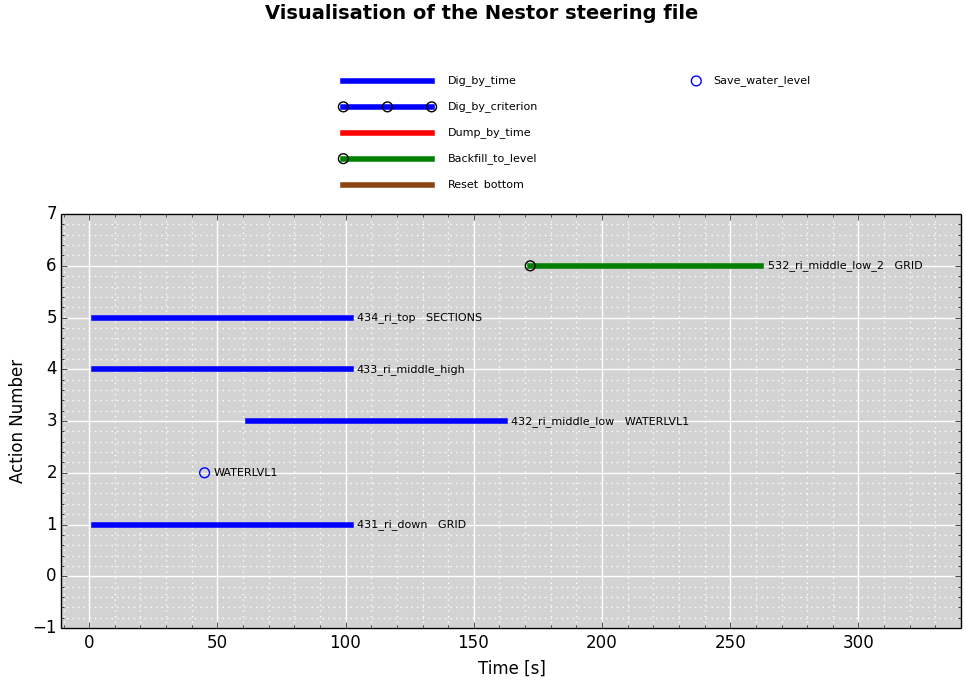
\includegraphics[width=0.95\textwidth]{img/TimeTableActions.png}
 \caption{Timetable of the actions.}
 \label{TiTa}
\end{figure}

\textcolor{white}{dummy line force dummy line by white lettering} %---- white line-----
\\
\\
%\\ \\
%\\ \\
%\\ \\
%\\ \\
% ******************************************************************
% **              DumpPlanar = TRUE/FALSE                         **
% ******************************************************************
\subsection{DumpPlanar details}\label{ssec:DumpPlanar}
\label{txt:DumpPlanar}
%
\textbf{Meaning of \texttt{DumpPlanar = TRUE} :}~~~The volume will be dumped only into the
lowest areas of the dump field. As a result all the nodes which were involved
will eventually have the same vertical distance to the reference surface.
In other words, after dumping the bottom locally has the shape as the reference level (fig.\,\ref{E4PlanT}).
The value of the distance will be calculated by Nestor due to the volume which is to dump.
If \texttt{DumpPlanar\,=\,TRUE} a reference level must be defined.
It's also possible to define a curved surface as reference level.
\begin{figure} [H]
 \centering
 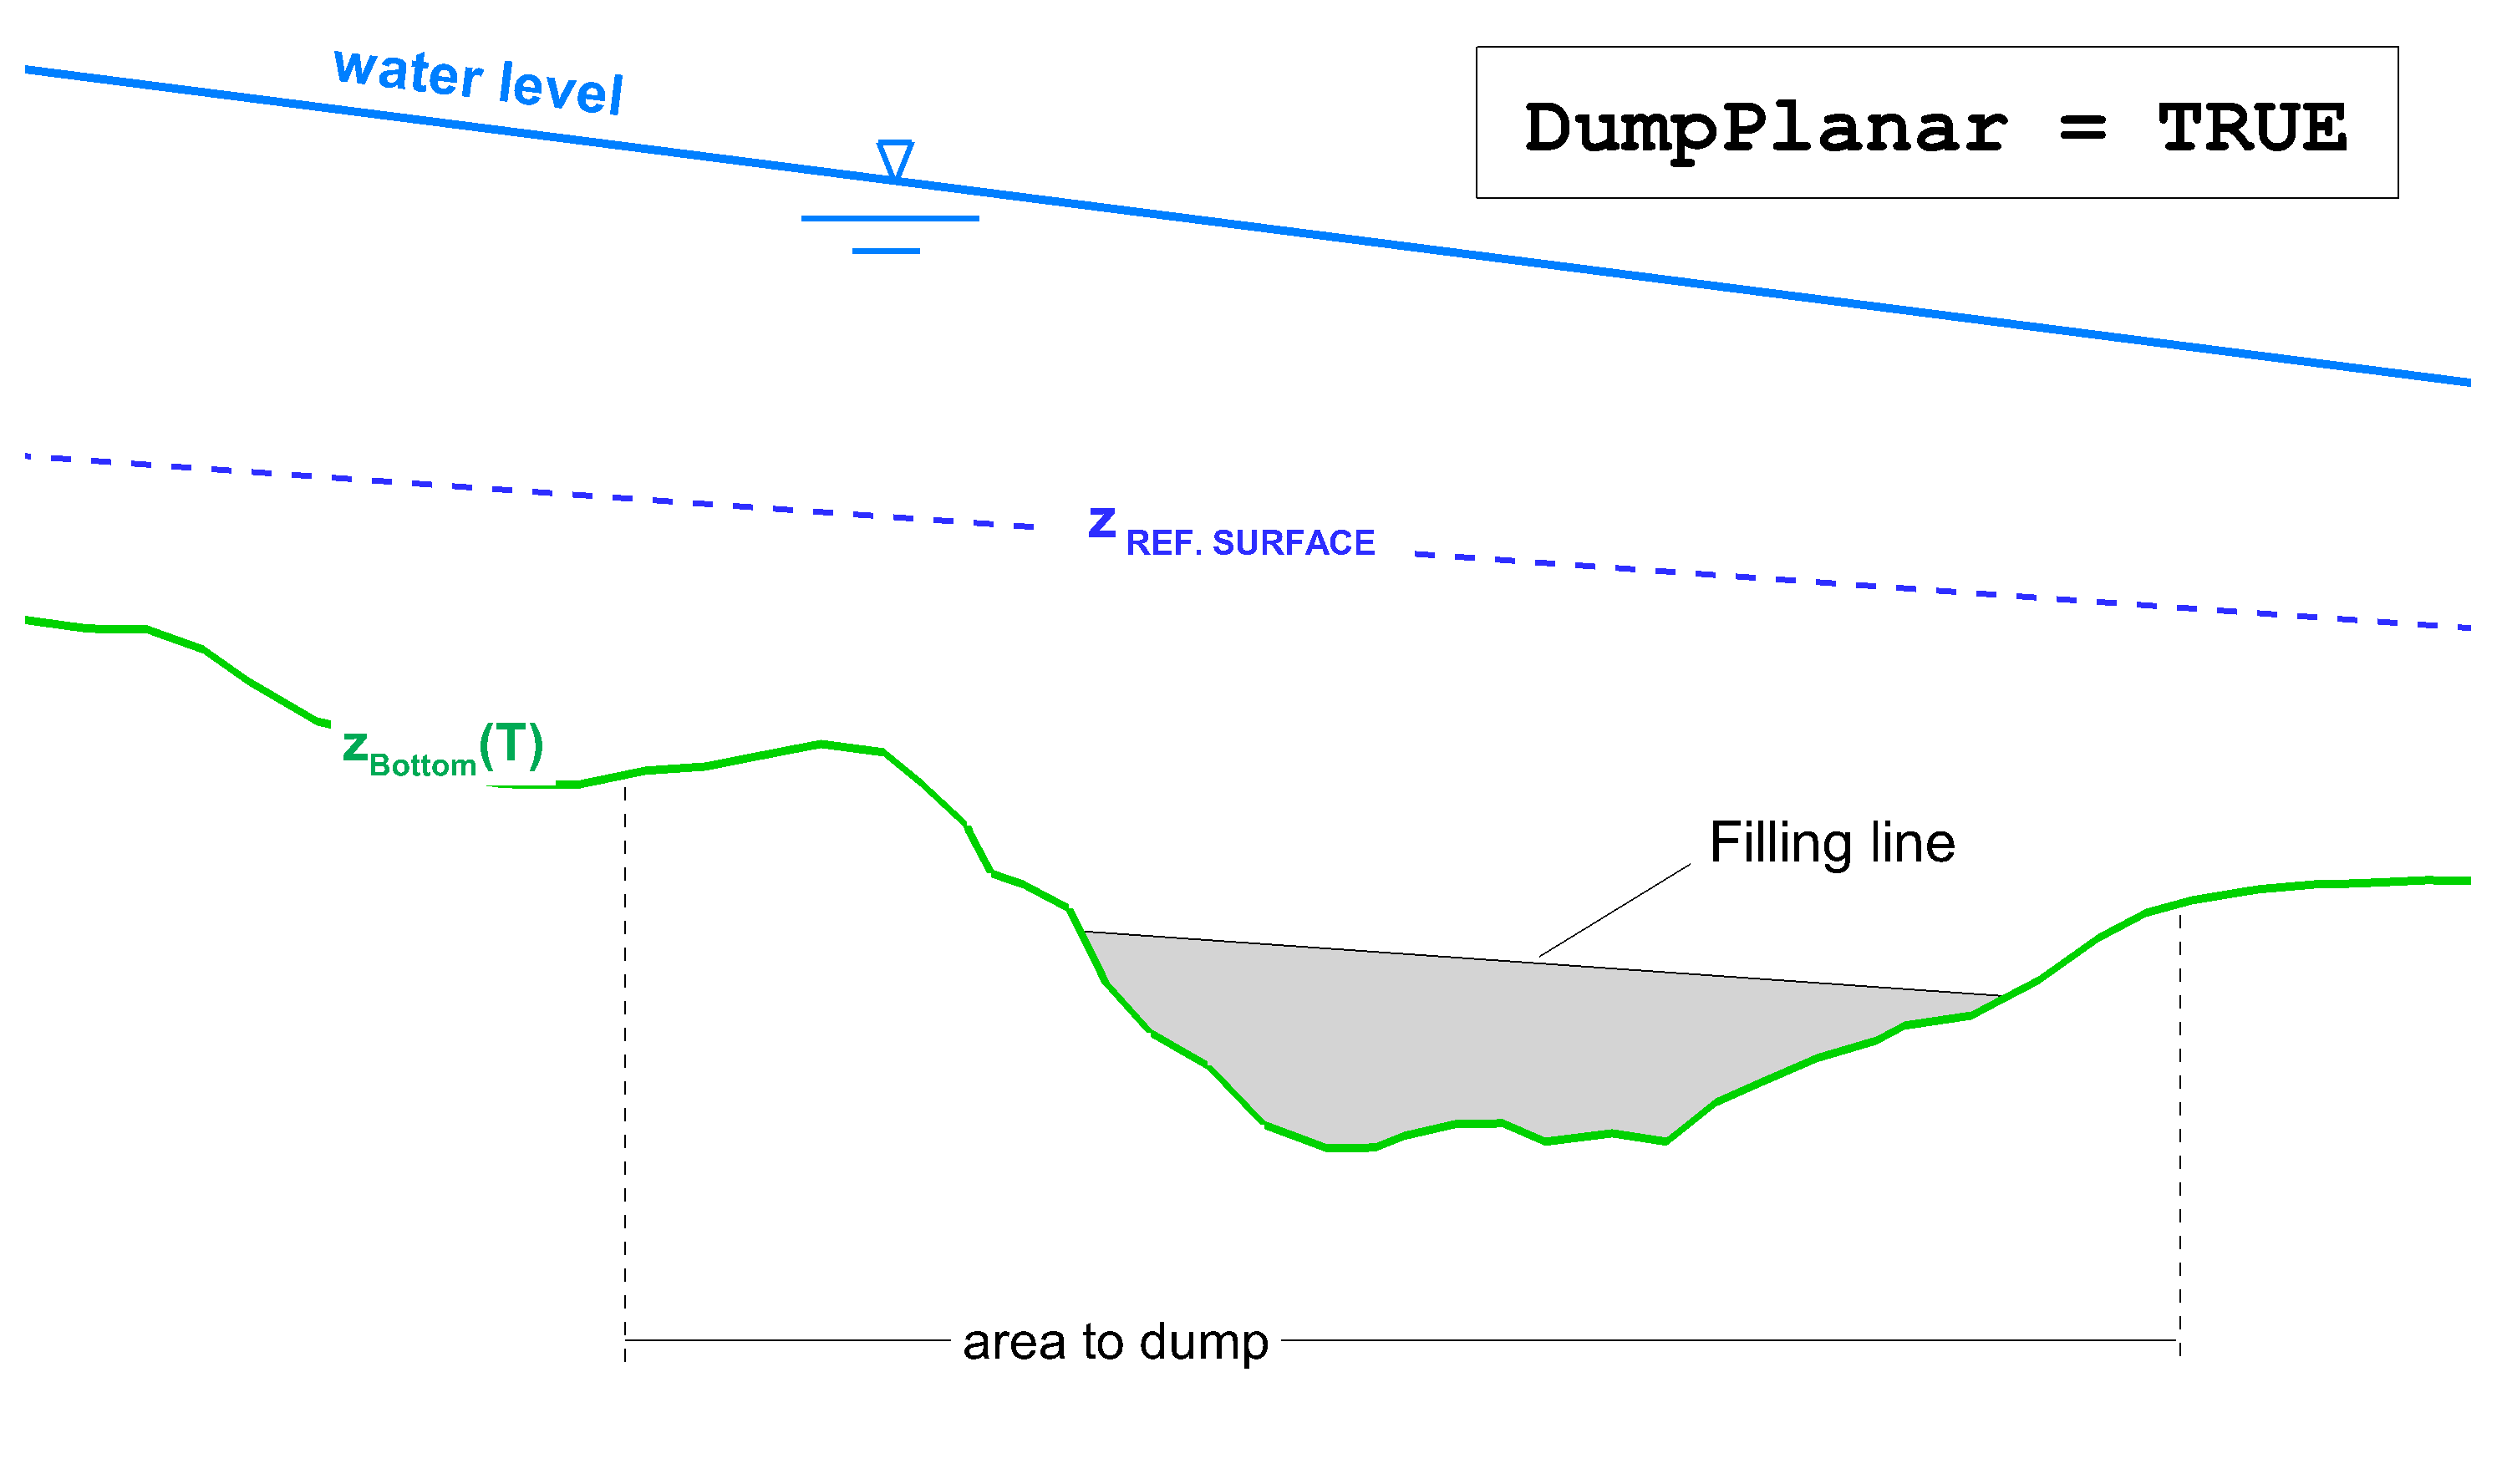
\includegraphics[scale=0.12]{img/Schema_DumpPlanar-true.png}
 \caption{Sheme how the bottom changes when the dump attribut \texttt{DumpPlanar\,=\,TRUE} is set.}
 \label{E4PlanT}
\end{figure}
%
\newpage
\textbf{Meaning of \texttt{DumpPlanar = FALSE} :}~~~A reference level is not used. Every node of
the dump field will be raised about the same amount (dz$_{\rm{per~node}}$ = const).
In other words, through the consistant dumping all over the entire field a layer of constant thickness
was added to the Bottom.(fig.\,\ref{E4PlanF})
\begin{figure} [H]
 \centering
 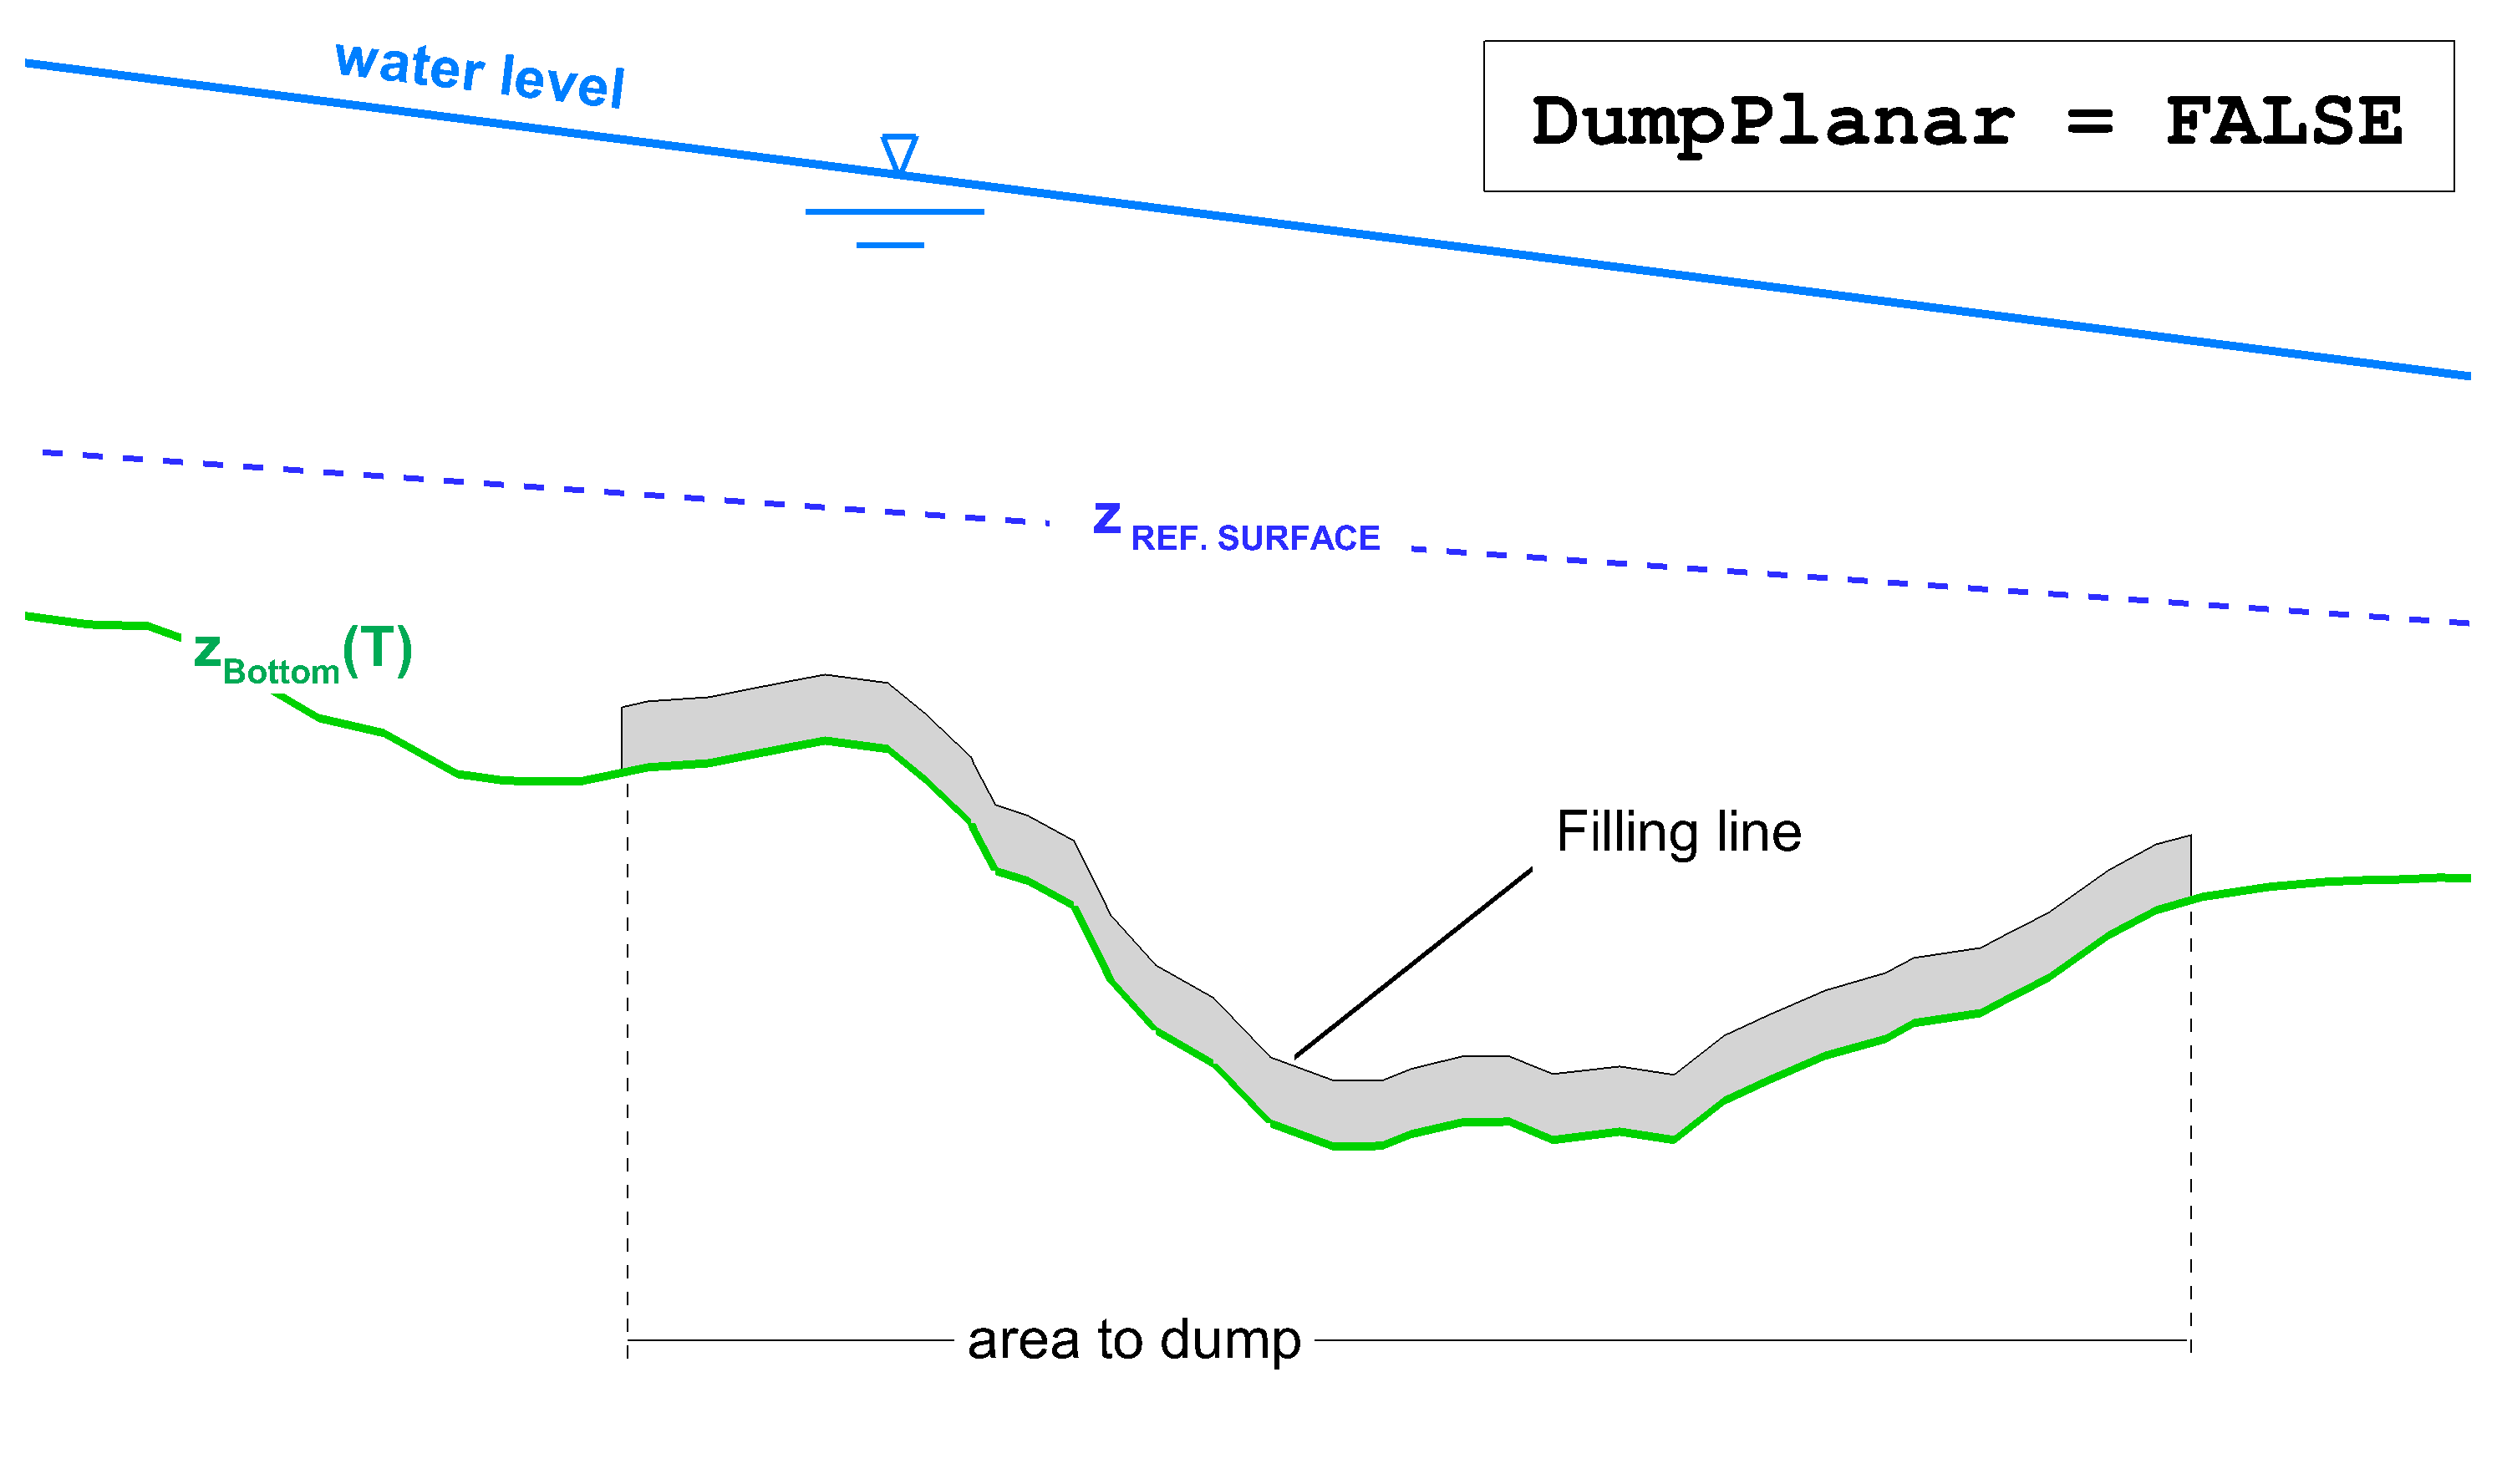
\includegraphics[scale=0.12]{img/Schema_DumpPlanar-false.png}
 \caption{Sheme how the bottom changes when the dump attribut \texttt{DumpPlanar\,=\,FALSE} is set.}
 \label{E4PlanF}
\end{figure}

\newpage
% ******************************************************************
% **                   Reference level                            **
% ******************************************************************
\subsection{Various kinds of Reference levels}\label{ssec:E4RefLev}
\label{txt:Reflevel}
%
There are three ways to define a reference level.
The specification is done in the action file.\\
\\
\fcolorbox{green}{yellow}{
\parbox{1.0\linewidth}{Conventions about the usage of a reference level:
\begin{itemize}
\item{A value for \texttt{~ReferenceLevel~} must be set only if \texttt{~DumpPlanar = TRUE} \\
      or \texttt{~Dig\_by\_criterion~} or \texttt{~Backfill\_to\_level~} is used.}
\item{The pre-defined values for keyword \texttt{~ReferenceLevel~} are:\\
      \texttt{GRID~;~SECTIONS~;~WATERLVL1~;~WATERLVL2~;~WATERLVL3~}}
\end{itemize}
}}

\begin{itemize}
  \itemsep20pt
  \item \texttt{ReferenceLevel = SECTIONS}:~~~define a surface by using sections
        (fig.\,\ref{refl3D} and \ref{geom2D}) which are stored in the file \texttt{\_DigRefLev.dat}
        (see page\,\pageref{txt:sectionFile})\\
  \item \texttt{ReferenceLevel = GRID}:~~~use the variable \texttt{REFERENCE LEVEL} in the \textsc{Geometry File}
        or \textsc{Previous Computation File} to specify a surface
        which is used as reference level (see grey surface in fig.\,\ref{refl3D}).
        (If coupled with sisyphe/gaia use \textsc{Previous Sedimentological Computation File}.)
  \item \texttt{ReferenceLevel = WATERLVL1}:~~~use a water level as reference level.
        \\The water level must be saved sometime before, before it can be used as reference level.
        Executing the action \texttt{Save\_water\_level} will save thels water level
        which was computed in the last time step. It's possible to use three different
        water levels at the same time. To address them use \texttt{WATERLVL1,WATERLVL2,WATERLVL3}
\end{itemize}

\begin{figure} [H]
  \centering
 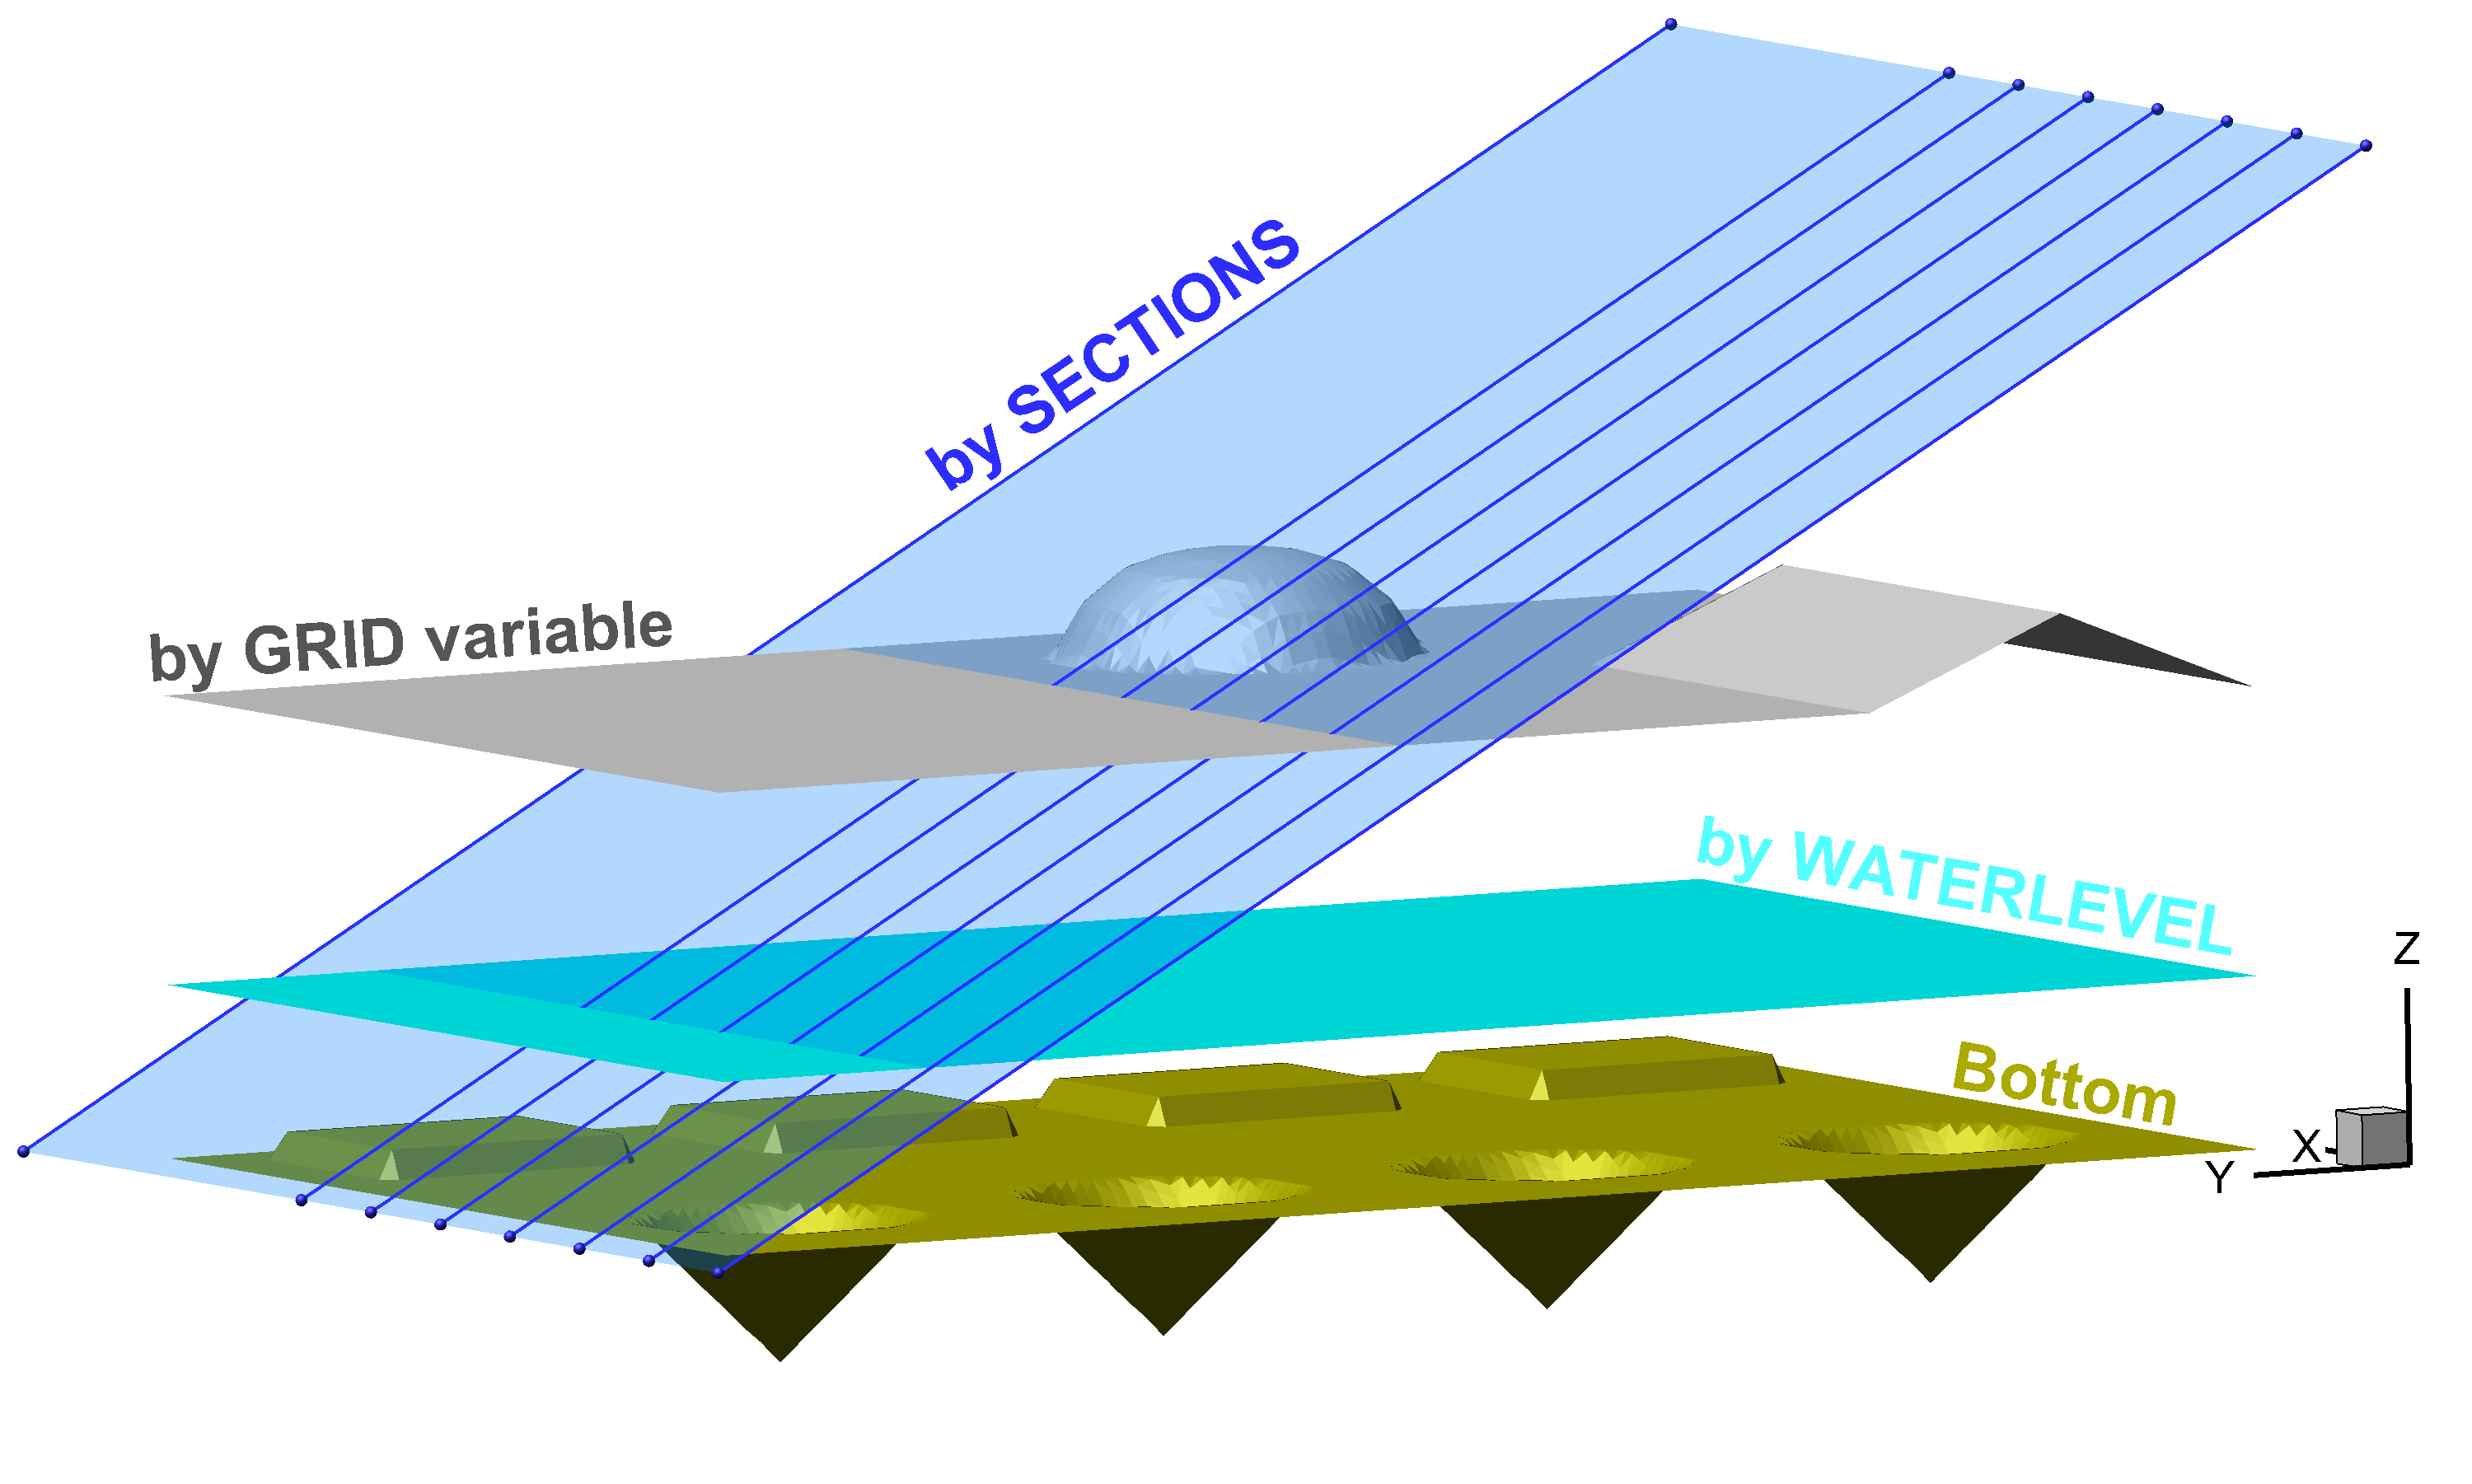
\includegraphics[scale=0.13]{img/Bild_Bottom_ZRL_3D_neu.png}
% \includegraphics[scale=0.16]{img/Bild_Bottom_ZRL_3D_wsp_Sek-neu_02.png}
% \includegraphics[scale=0.13]{img/Bild_Bottom_ZRL_3D_wsp_Sek-neu_02.png}
  \caption{Initial bottom geometry, various reference levels defined through sections, through a waterlevel and
  through a grid variable (vertical exaggeration 2x)}
  \label{refl3D}
\end{figure}

\newpage
\begin{figure} [H]
 \centering
 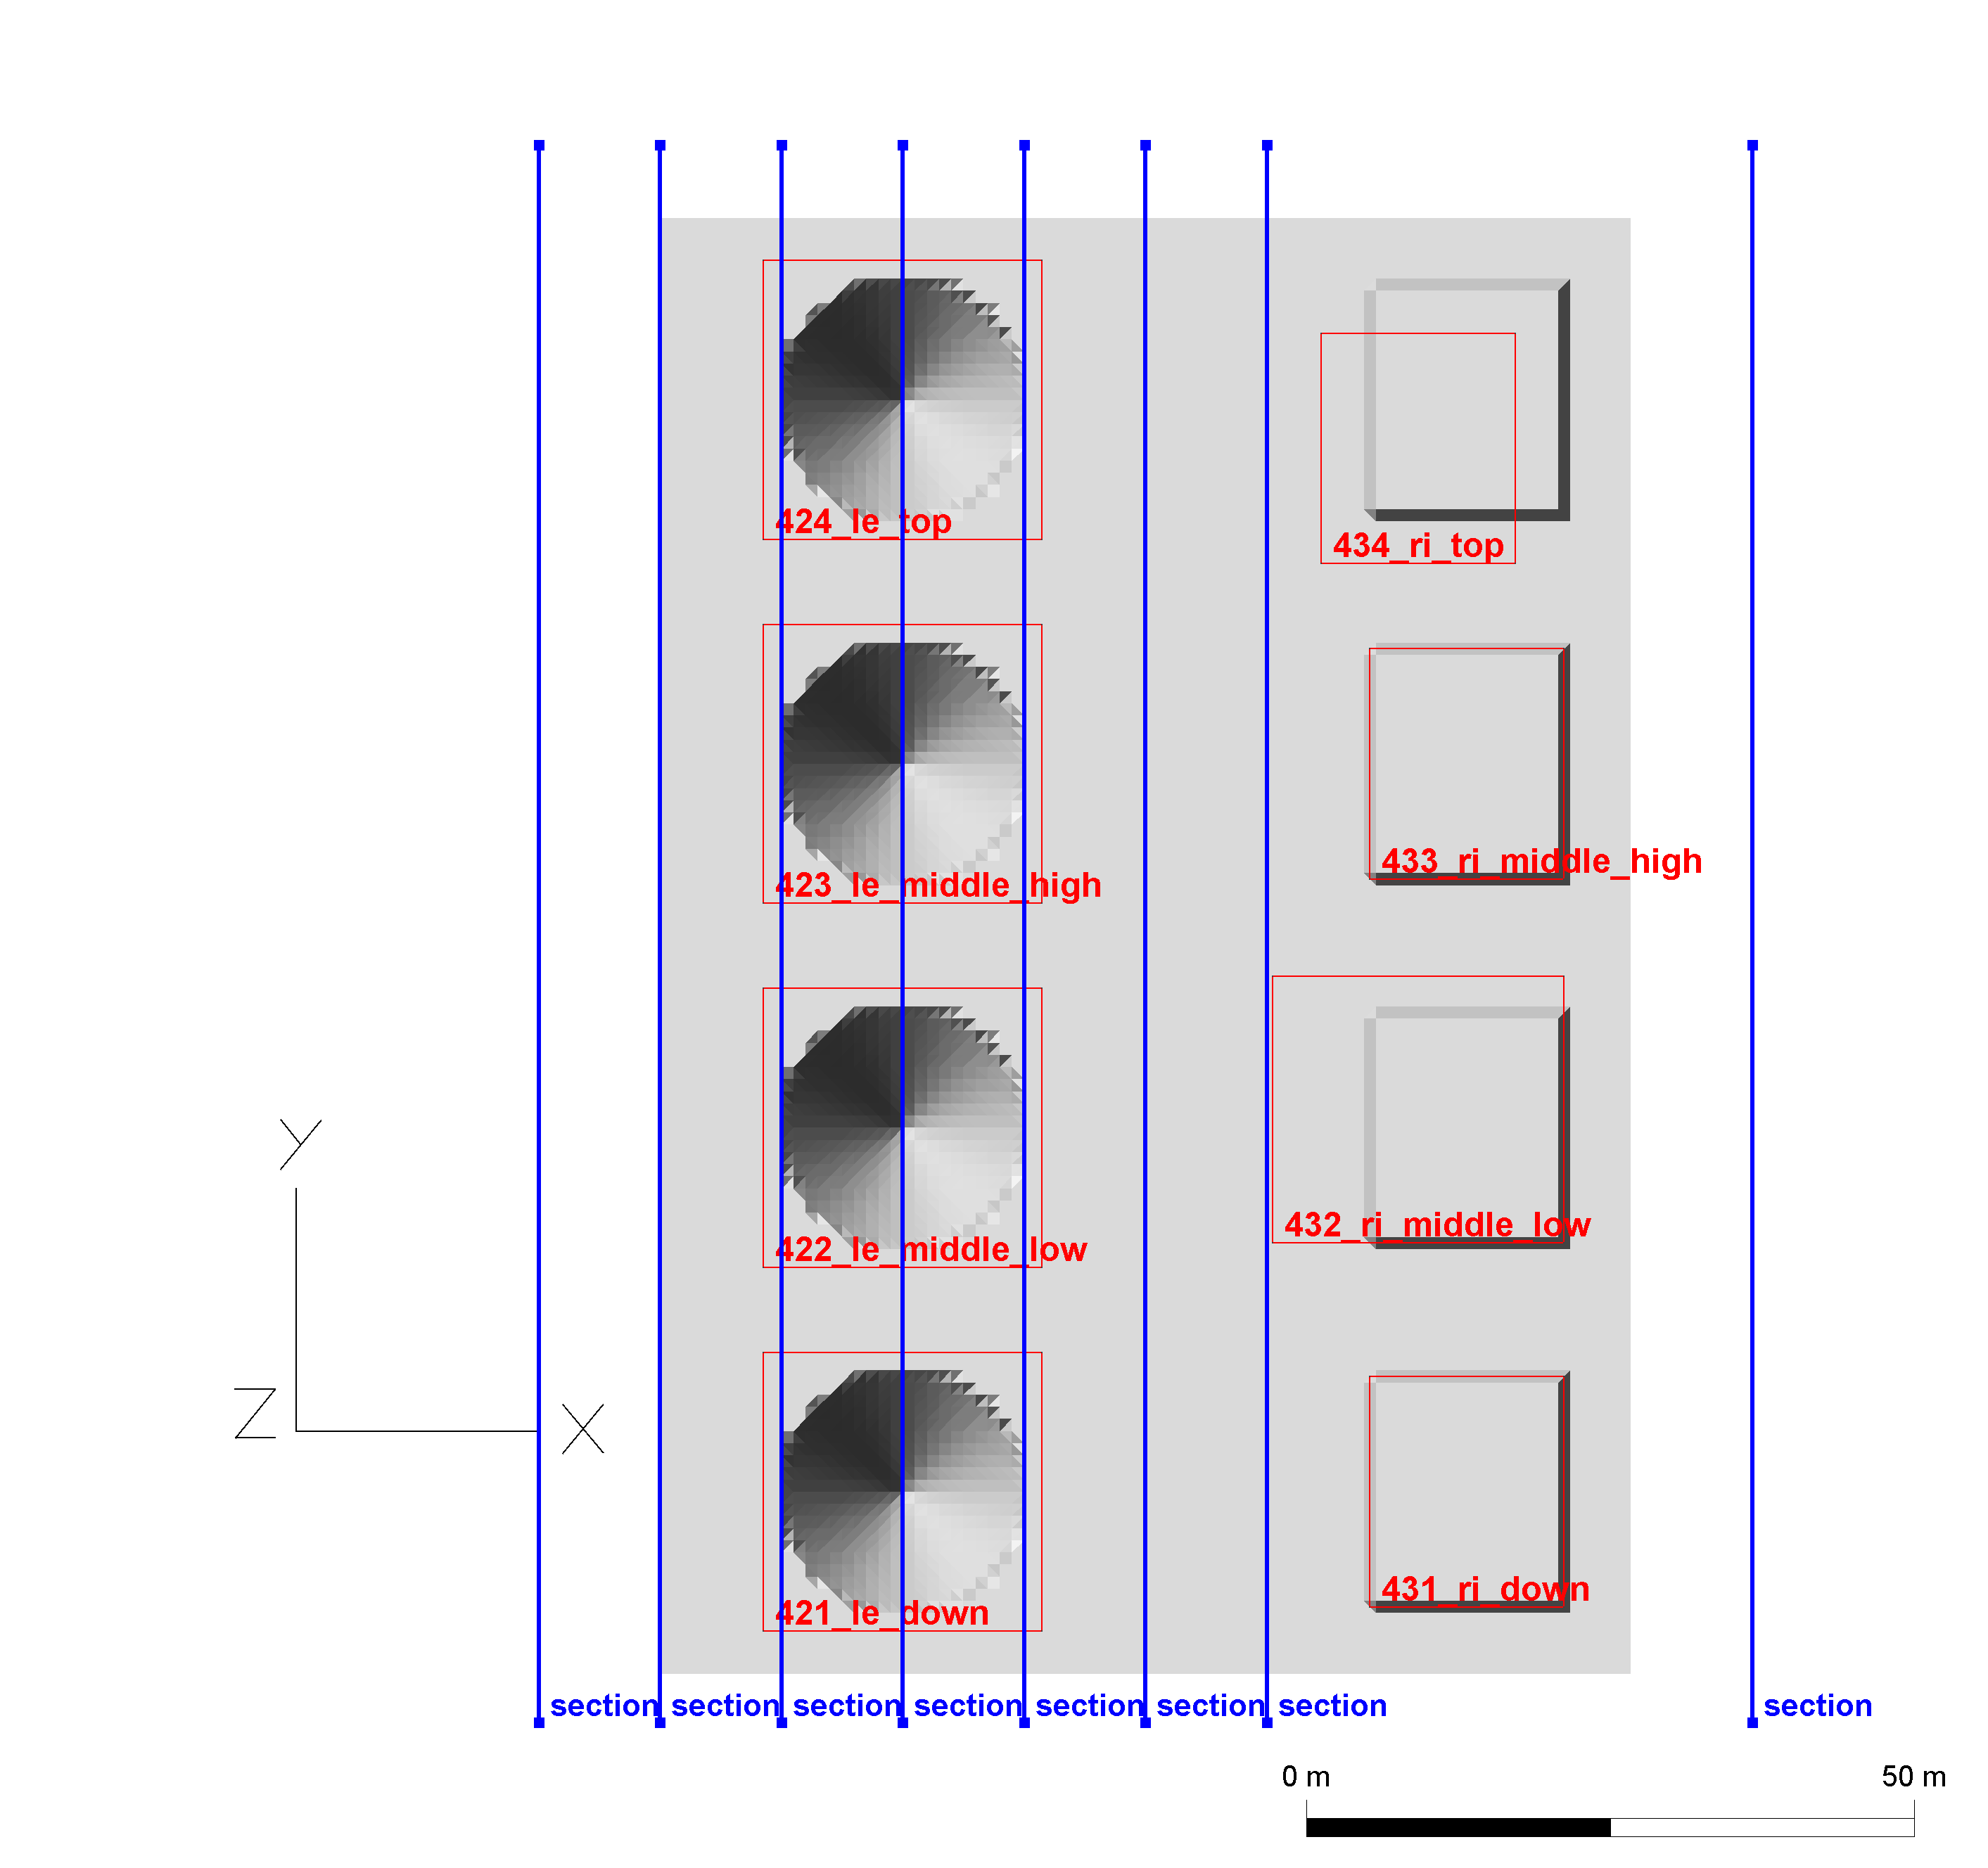
\includegraphics[scale=0.15]{img/Bild_4cones_Lageplan_DigPoly_Sections_2D.png}
 \caption{Initial bottom geometry, polygons to define the dredging and dumping fields
  and sections to define a reference level}
 \label{geom2D}
\end{figure}

\label{txt:sectionFile}
Excerpt of the reference level file \texttt{\_DigRefLev.dat}: \label{txt:E4RefLevFile}
\\
\\ \hspace*{3mm} \texttt{\scriptsize{\#  comment line                                            }}
\\ \hspace*{3mm} \texttt{\scriptsize{\#~~~xL~~~~~yL~~~~~zL~~~~~~~~~xR~~~~yR~~~~~zR~~~~~~~flow length}}
\\ \hspace*{3mm} \texttt{\scriptsize{~~100.0~~~116.0~~0.00~~~~~~100.0~~79.0~~10.00~~~~~~~~~0.100 }}
\\ \hspace*{3mm} \texttt{\scriptsize{~~110.0~~~116.0~~0.00~~~~~~110.0~~79.0~~10.00~~~~~~~~~0.110 }}
\\ \hspace*{3mm} \texttt{\scriptsize{~~  ....                                                    }}
\\ \hspace*{3mm} \texttt{\scriptsize{~~150.0~~~116.0~~0.00~~~~~~150.0~~79.0~~10.00~~~~~~~~~0.150 }}
\\ \hspace*{3mm} \texttt{\scriptsize{~~160.0~~~116.0~~0.00~~~~~~160.0~~79.0~~10.00~~~~~~~~~0.160 }}
\\ \hspace*{3mm} \texttt{\scriptsize{END                                                         }}



% ******************************************************************
% ******************************************************************
% **                                                              **
% **                          Action-1                            **
% ******************************************************************
% ******************************************************************
\newpage
\subsection{Action-1: ActionType\, = \,Dig\_by\_time , ReferenceLevel = GRID}
\label{ssec:E4Action1}
\textbf{Action-1 :}~~~\texttt{ActionType\,=\,Dig\_by\_time:}~~~In the flield \texttt{431\_ri\_down} a
volume of 300\,m$^3$ will be dredged during a time slot of 100\,s.
The time slot begins at simulation time 00:00:02 (hh:mm:ss).
As a result every node in the field will be lowered by 0.987\,m (fig.\,\ref{Act1}c).
Simultaneously the dredged material will be dumped into the lower areas of the field \texttt{421\_le\_down}.
If there would be no setting for \texttt{FieldDump} the dredged volume would not be dumped.
Because of the setting \texttt{DumpRate=0.045}, the pacing of dumping is limited and
takes 140\,s to dump all of the dredged volume (fig.\,\ref{Act1}d).
Consequently Nestor is still dumping even though the dredging is finished.\\
%To find some information about:
%\\ \hspace*{3mm} - when the action was active and
%\\ \hspace*{3mm} - what was going on,\\
%search in the telemac outputfile (\texttt{validateNestor4.out????}) for lines with \texttt{"?>"} at the beginning.\\
Because of the setting \texttt{DumpPlanar=TRUE} and \texttt{ReferenceLevel=GRID} the surface which is available
in the \textsc{Geometry File} is used as reference level.
The bottom where the dumping happened is shaped like a roof referring to the shape of
the reference level above the dump field (grey surface in fig.\,\ref{refl3D}).\\
\\
\\
Excerpt from the action file where the Action-1 is defined:
\\ \hspace*{3mm} \texttt{\small{/================================================================}}
\\ \hspace*{3mm} \texttt{\small{ACTION}}
\\ \hspace*{3mm} \texttt{\small{~~ActionType~~~~~~=~Dig\_by\_time}}
\\ \hspace*{3mm} \texttt{\small{~~ReferenceLevel~~=~~GRID}}
\\ \hspace*{3mm} \texttt{\small{~~TimeStart~~~~~~~=~~2000.01.01-00:00:02~~/~[yyyy.mm.dd-hh:mm:ss]}}
\\ \hspace*{3mm} \texttt{\small{~~TimeEnd~~~~~~~~~=~~2000.01.01-00:01:42~~/~[yyyy.mm.dd-hh:mm:ss]}}
\\ \hspace*{3mm}
\\ \hspace*{3mm} \texttt{\small{~~FieldDig~~~~~~~~=~~431\_ri\_down}}
\\ \hspace*{3mm} \texttt{\small{~~DigVolume~~~~~~~=~~300.0~~~~~~~~~~~~~~~~/~[m\textasciicircum3]}}
\\ \hspace*{3mm}
\\ \hspace*{3mm} \texttt{\small{~~FieldDump~~~~~~~=~~421\_le\_down}}
\\ \hspace*{3mm} \texttt{\small{~~DumpPlanar~~~~~~=~~TRUE}}
\\ \hspace*{3mm} \texttt{\small{~~DumpRate~~~~~~~~=~~0.045~~~~~~~~~~~~~~~~/~[m/s]}}
\\ \hspace*{3mm} \texttt{\small{ENDACTION}}
\\ \hspace*{3mm} \texttt{\small{/================================================================}}
\\
\\
\\
\\
\\
\\
\\
\\
\textcolor{white}{dummy line force dummy line by white lettering} %---- white line-----


\begin{figure}[H]
  \centering
    \subfloat[]                    {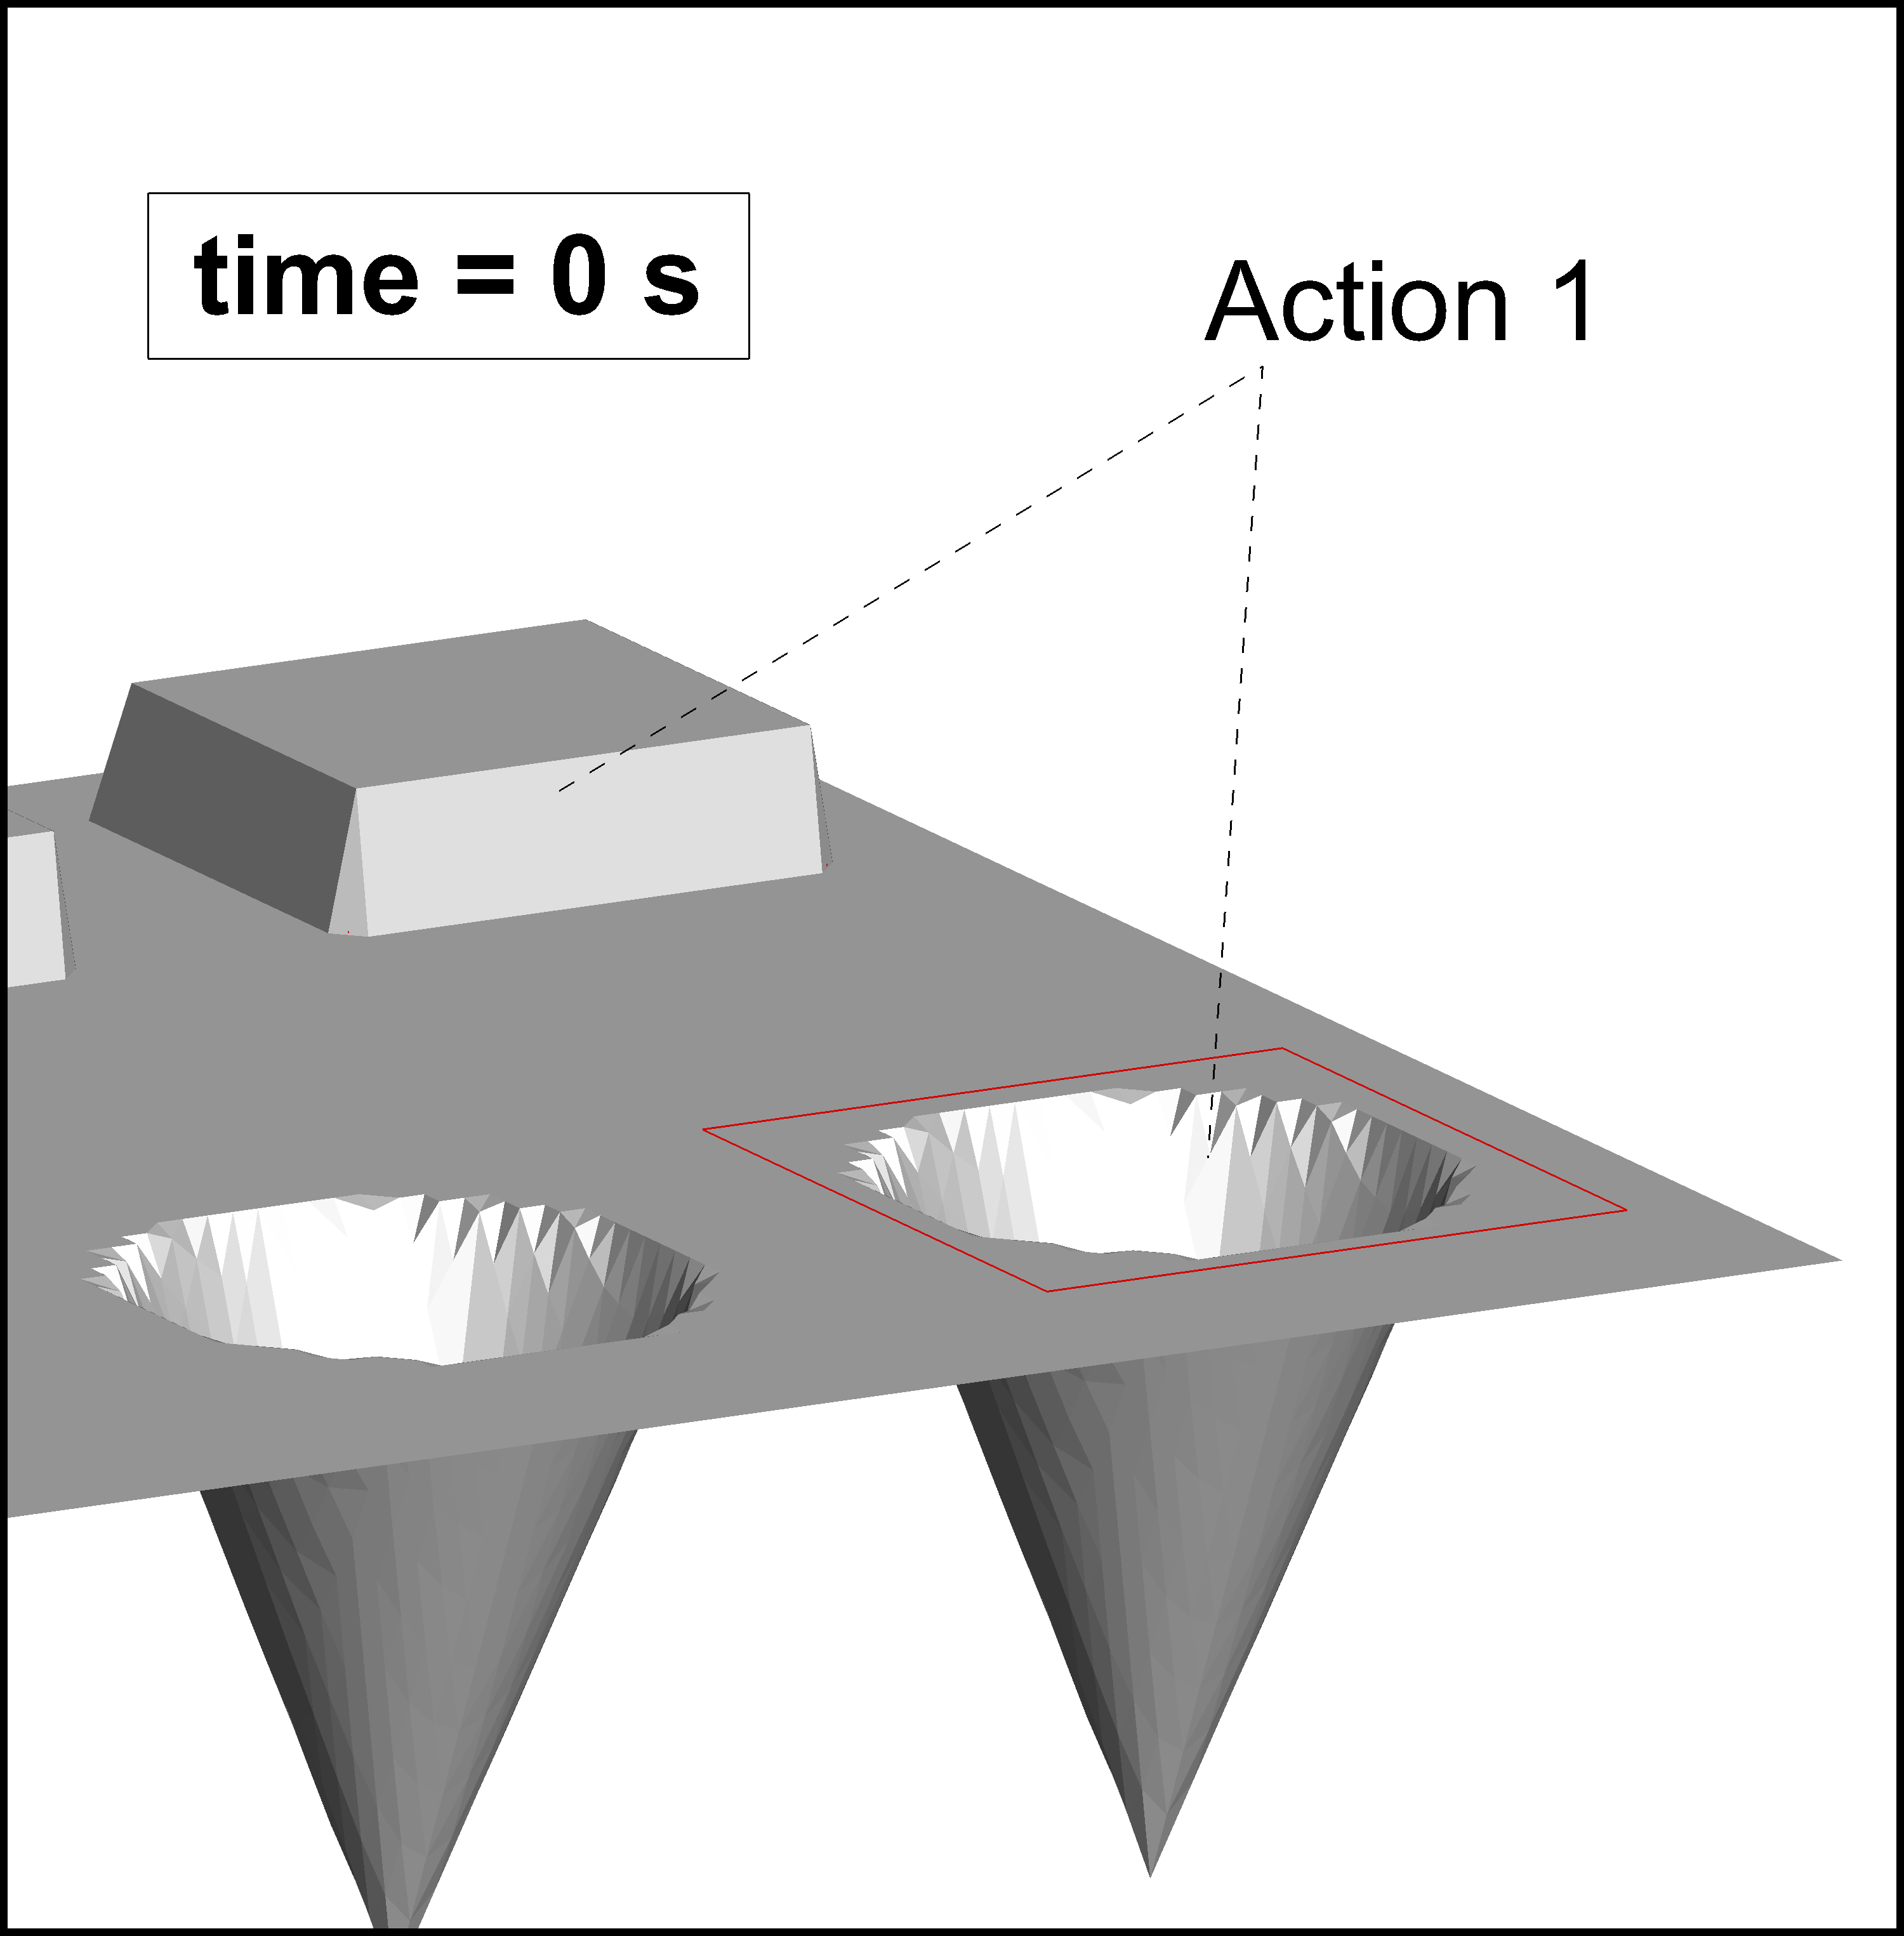
\includegraphics[width=0.45\textwidth]{img/Bild_Act1_000s.png}}\qquad
    \subfloat[dredging and dumping]{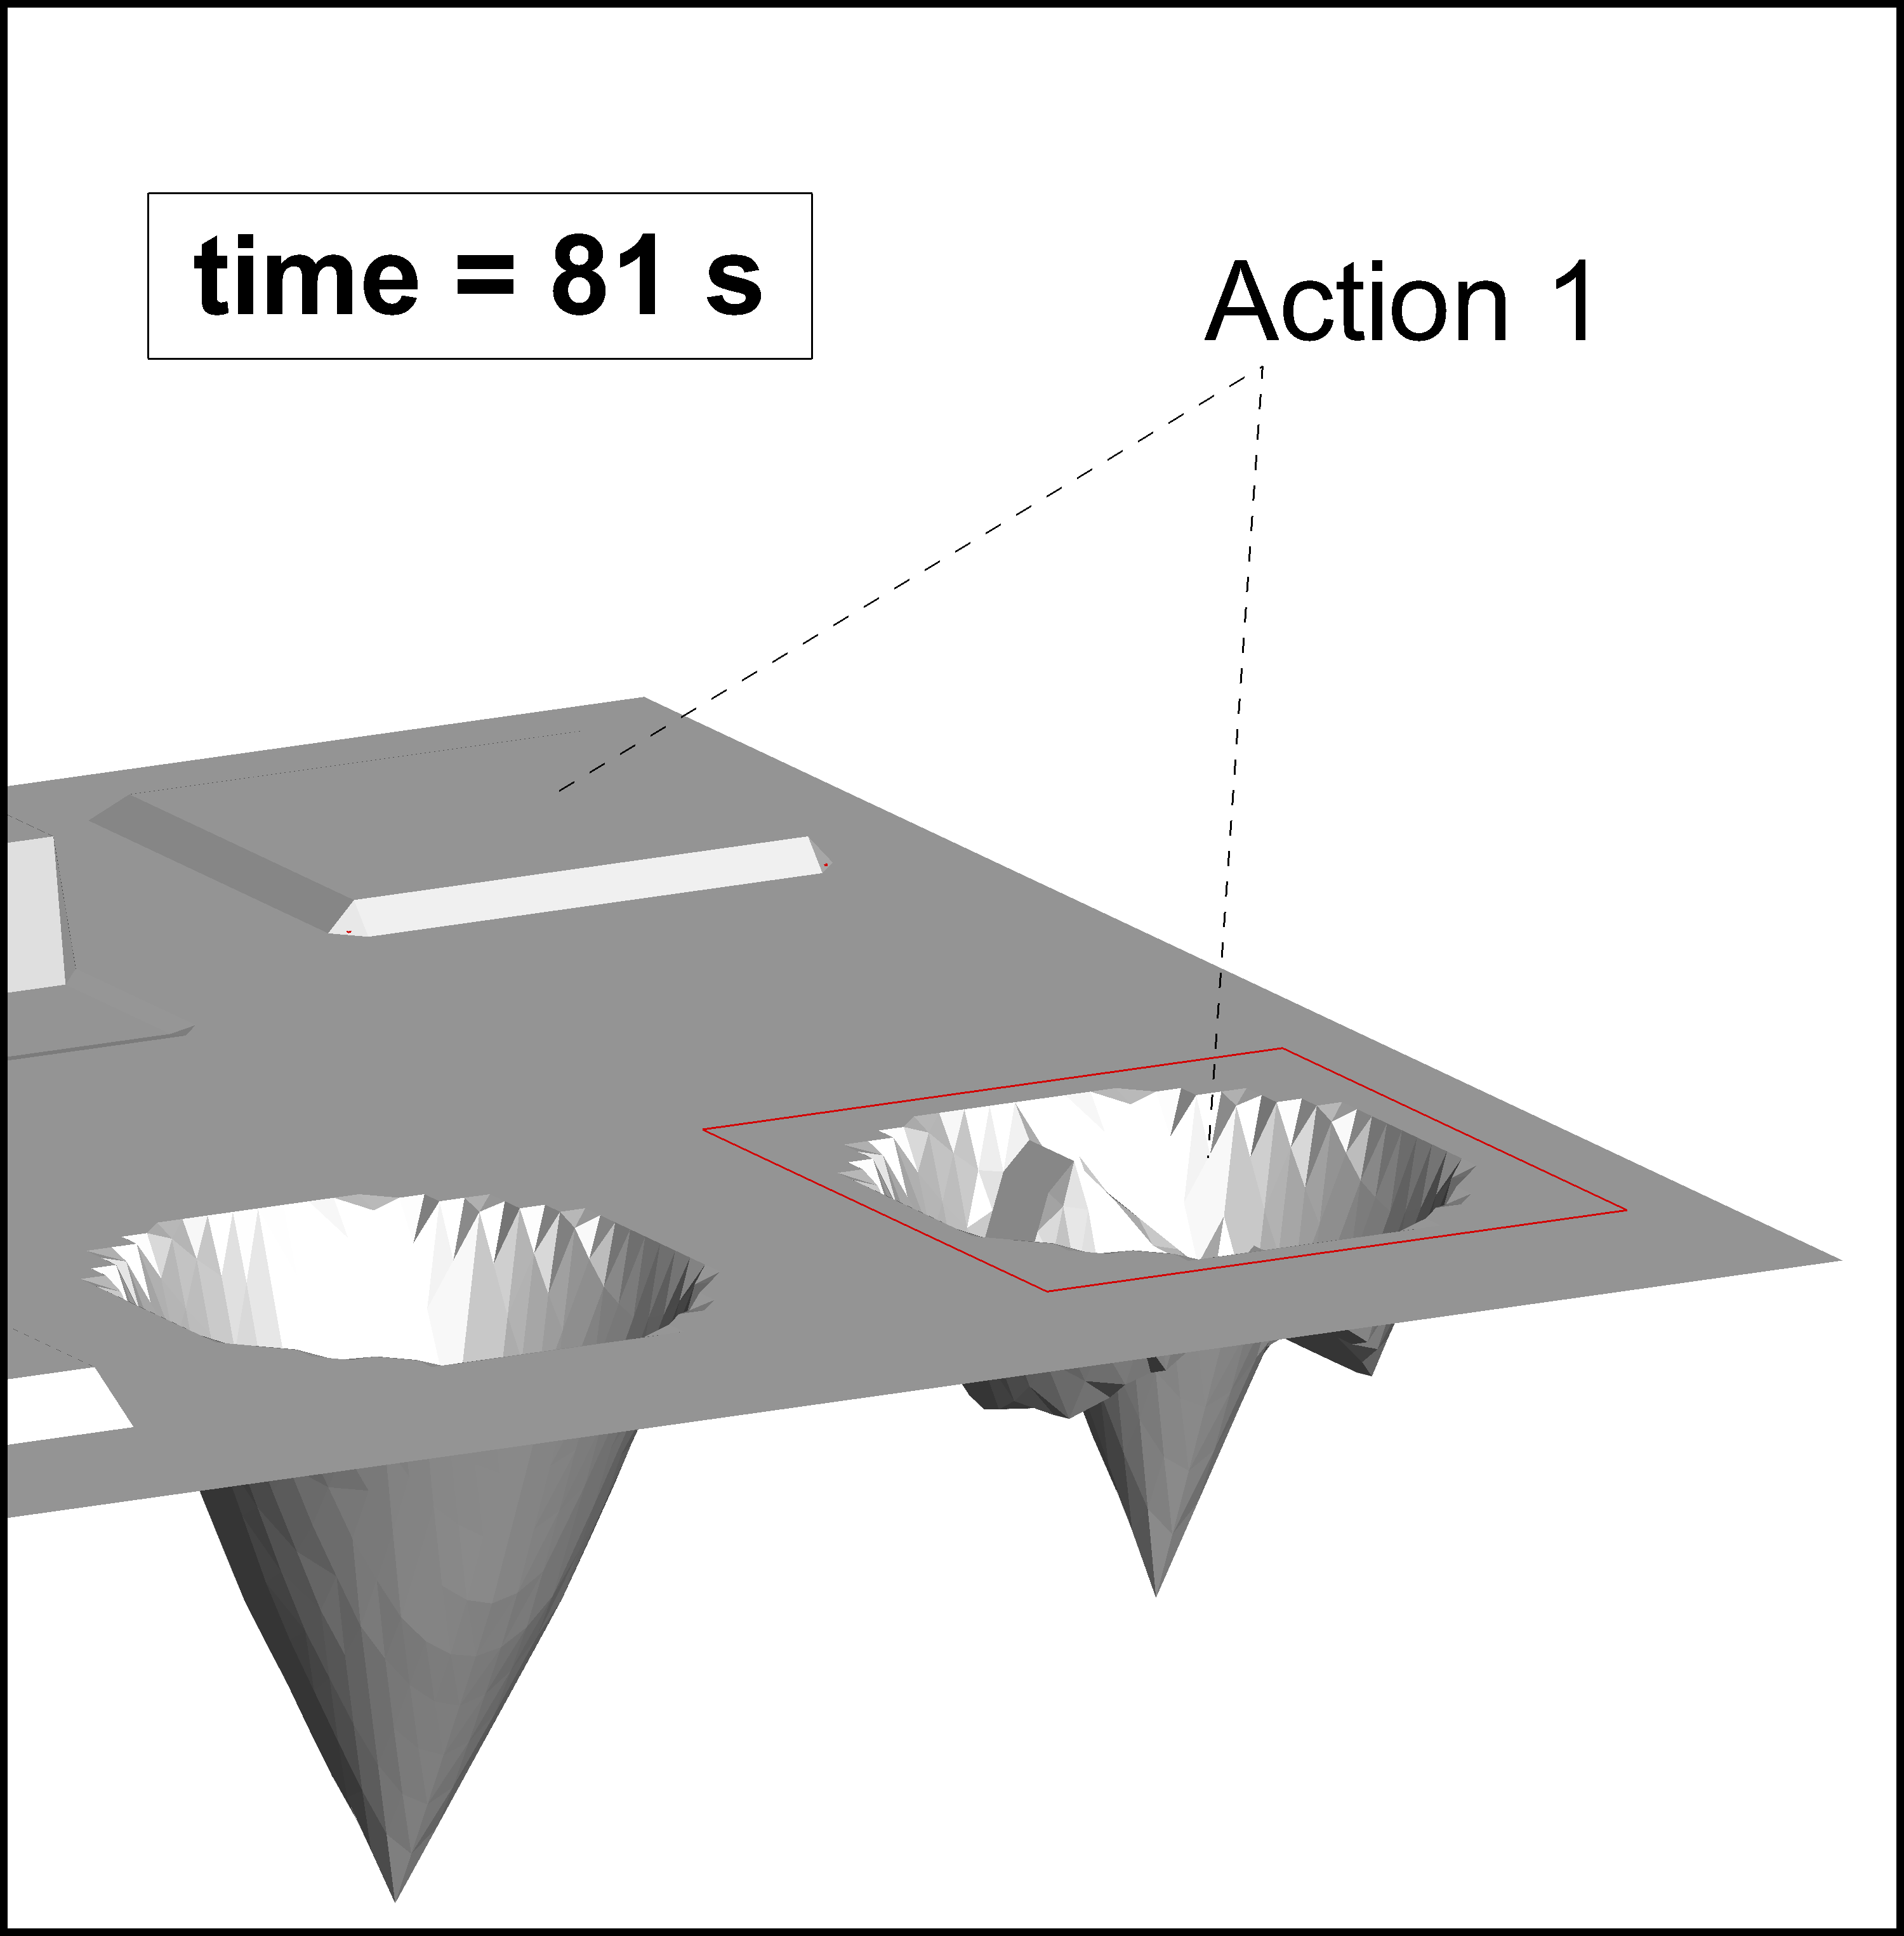
\includegraphics[width=0.45\textwidth]{img/Bild_Act1_081s.png}}\qquad
    \subfloat[dredging just  finished,
                     still dumping]{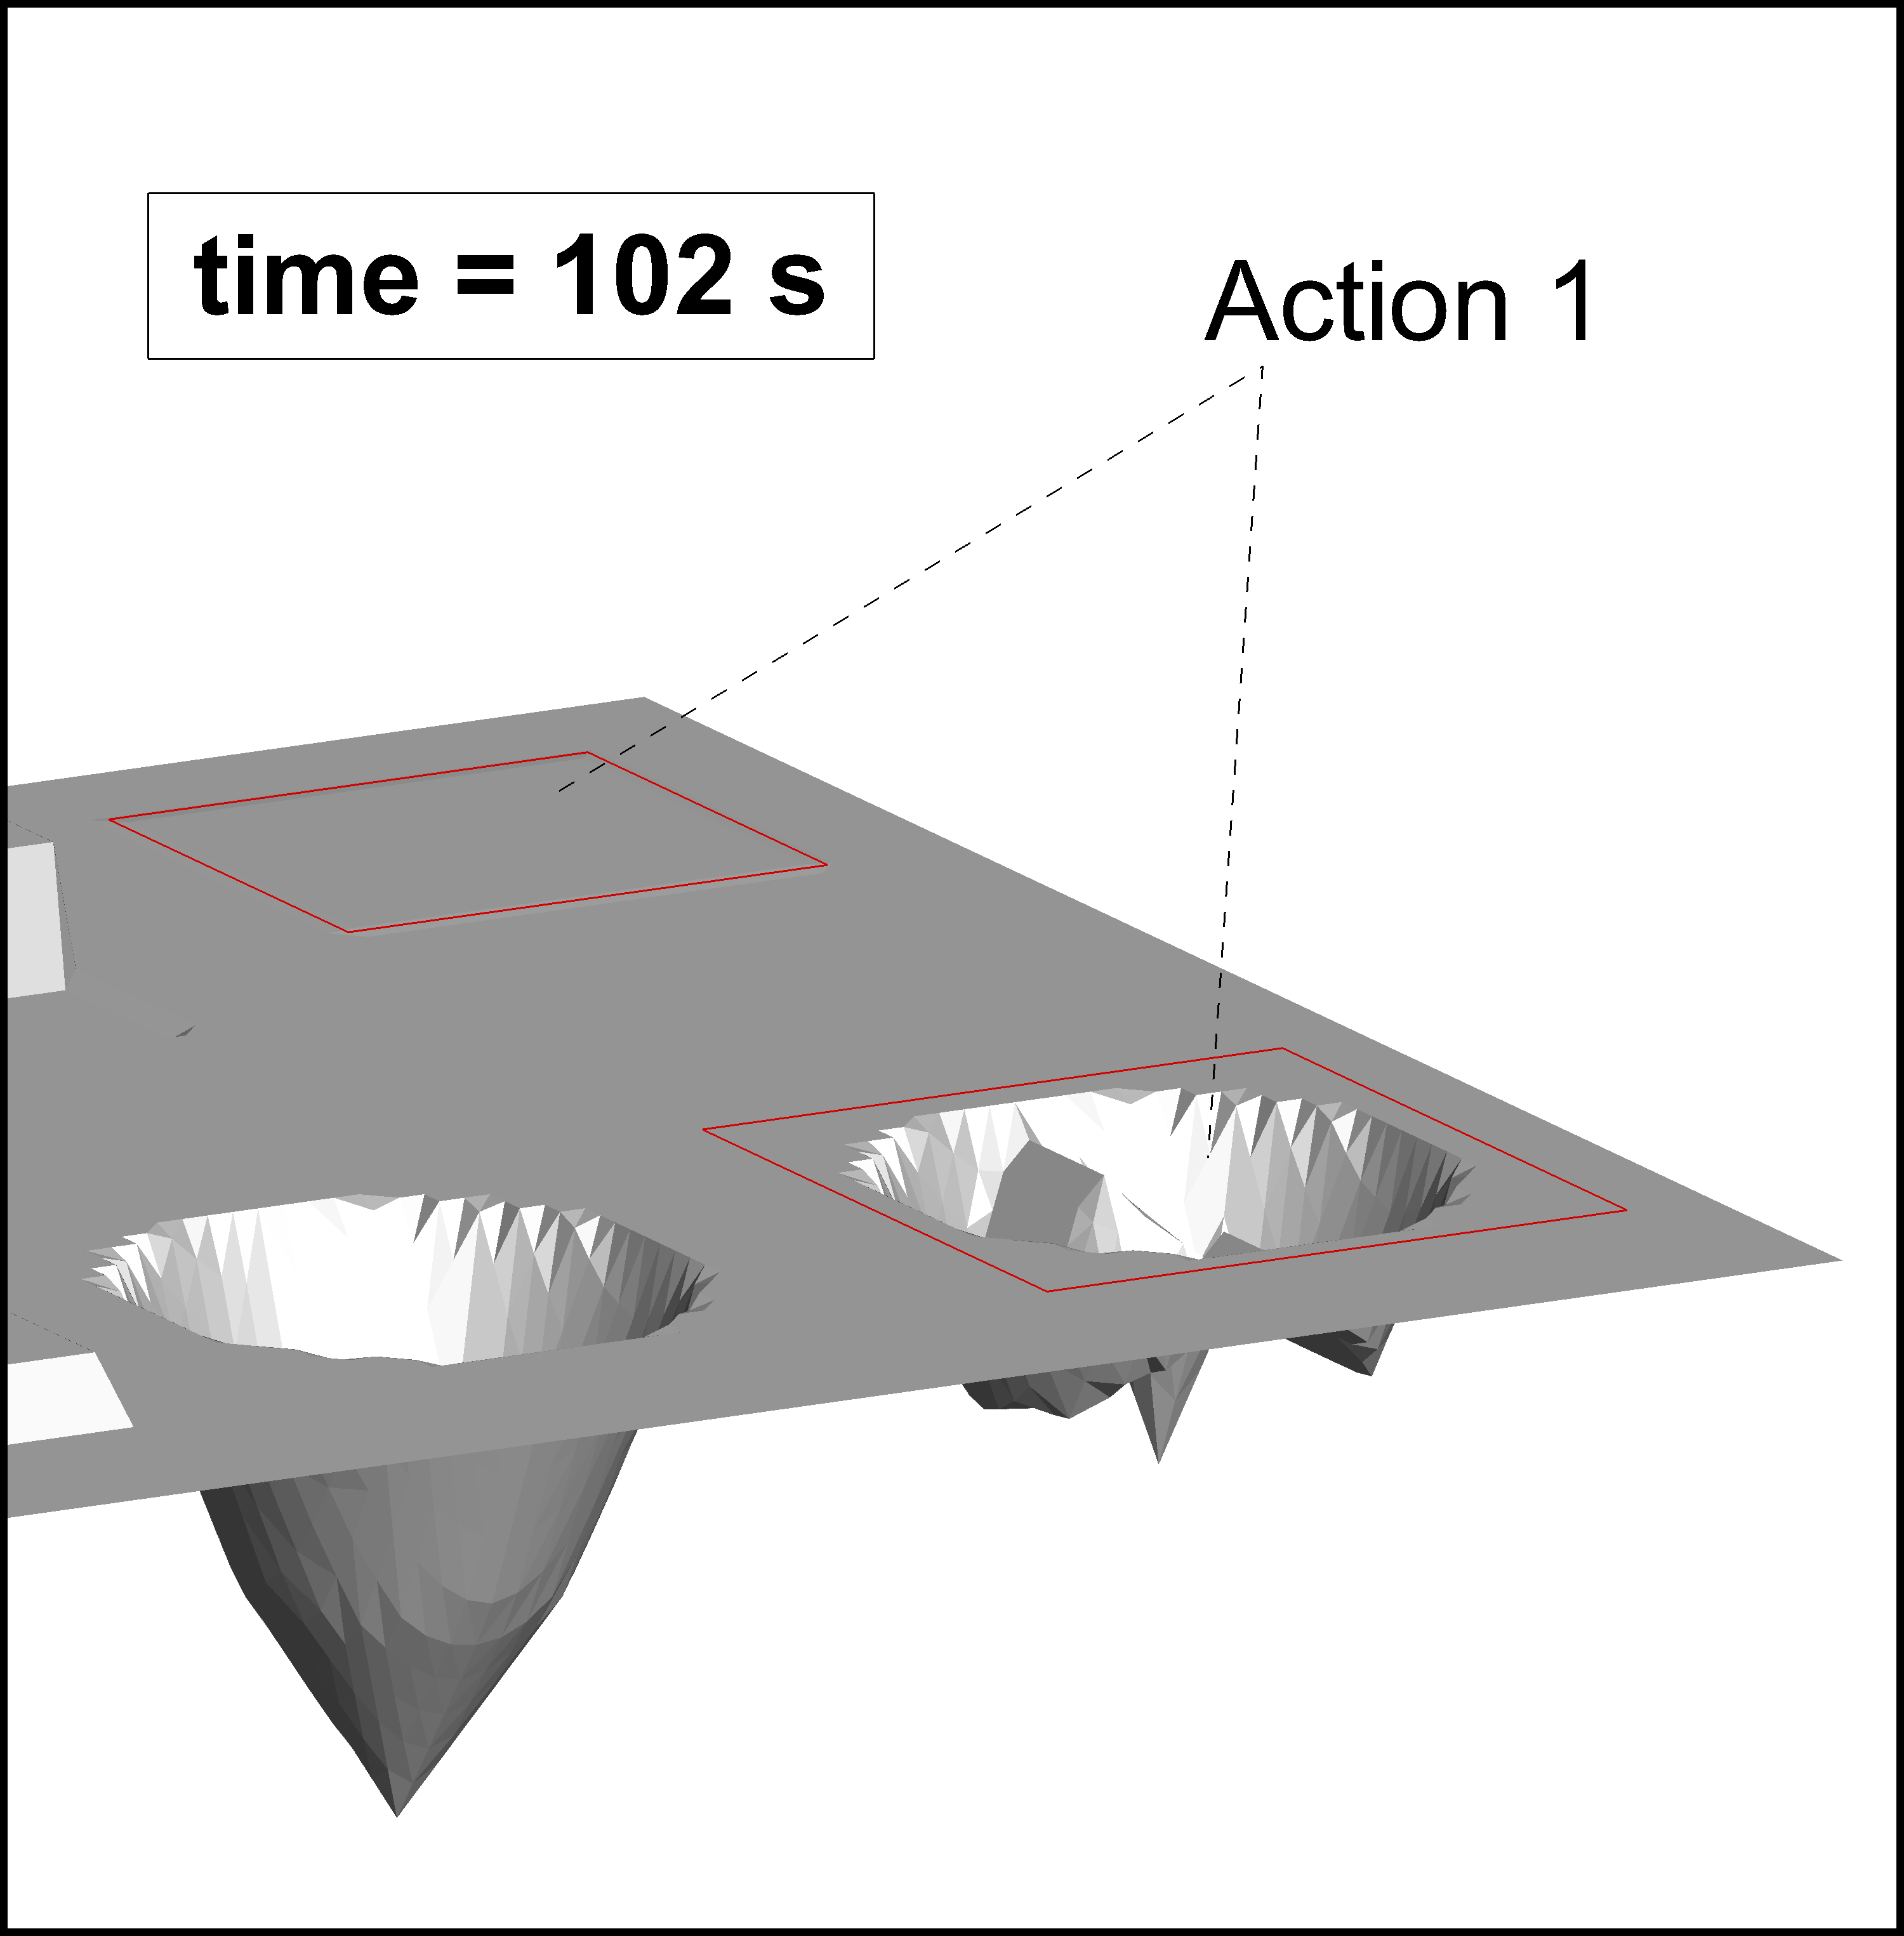
\includegraphics[width=0.45\textwidth]{img/Bild_Act1_102s.png}}\qquad
    \subfloat[dumping finished]    {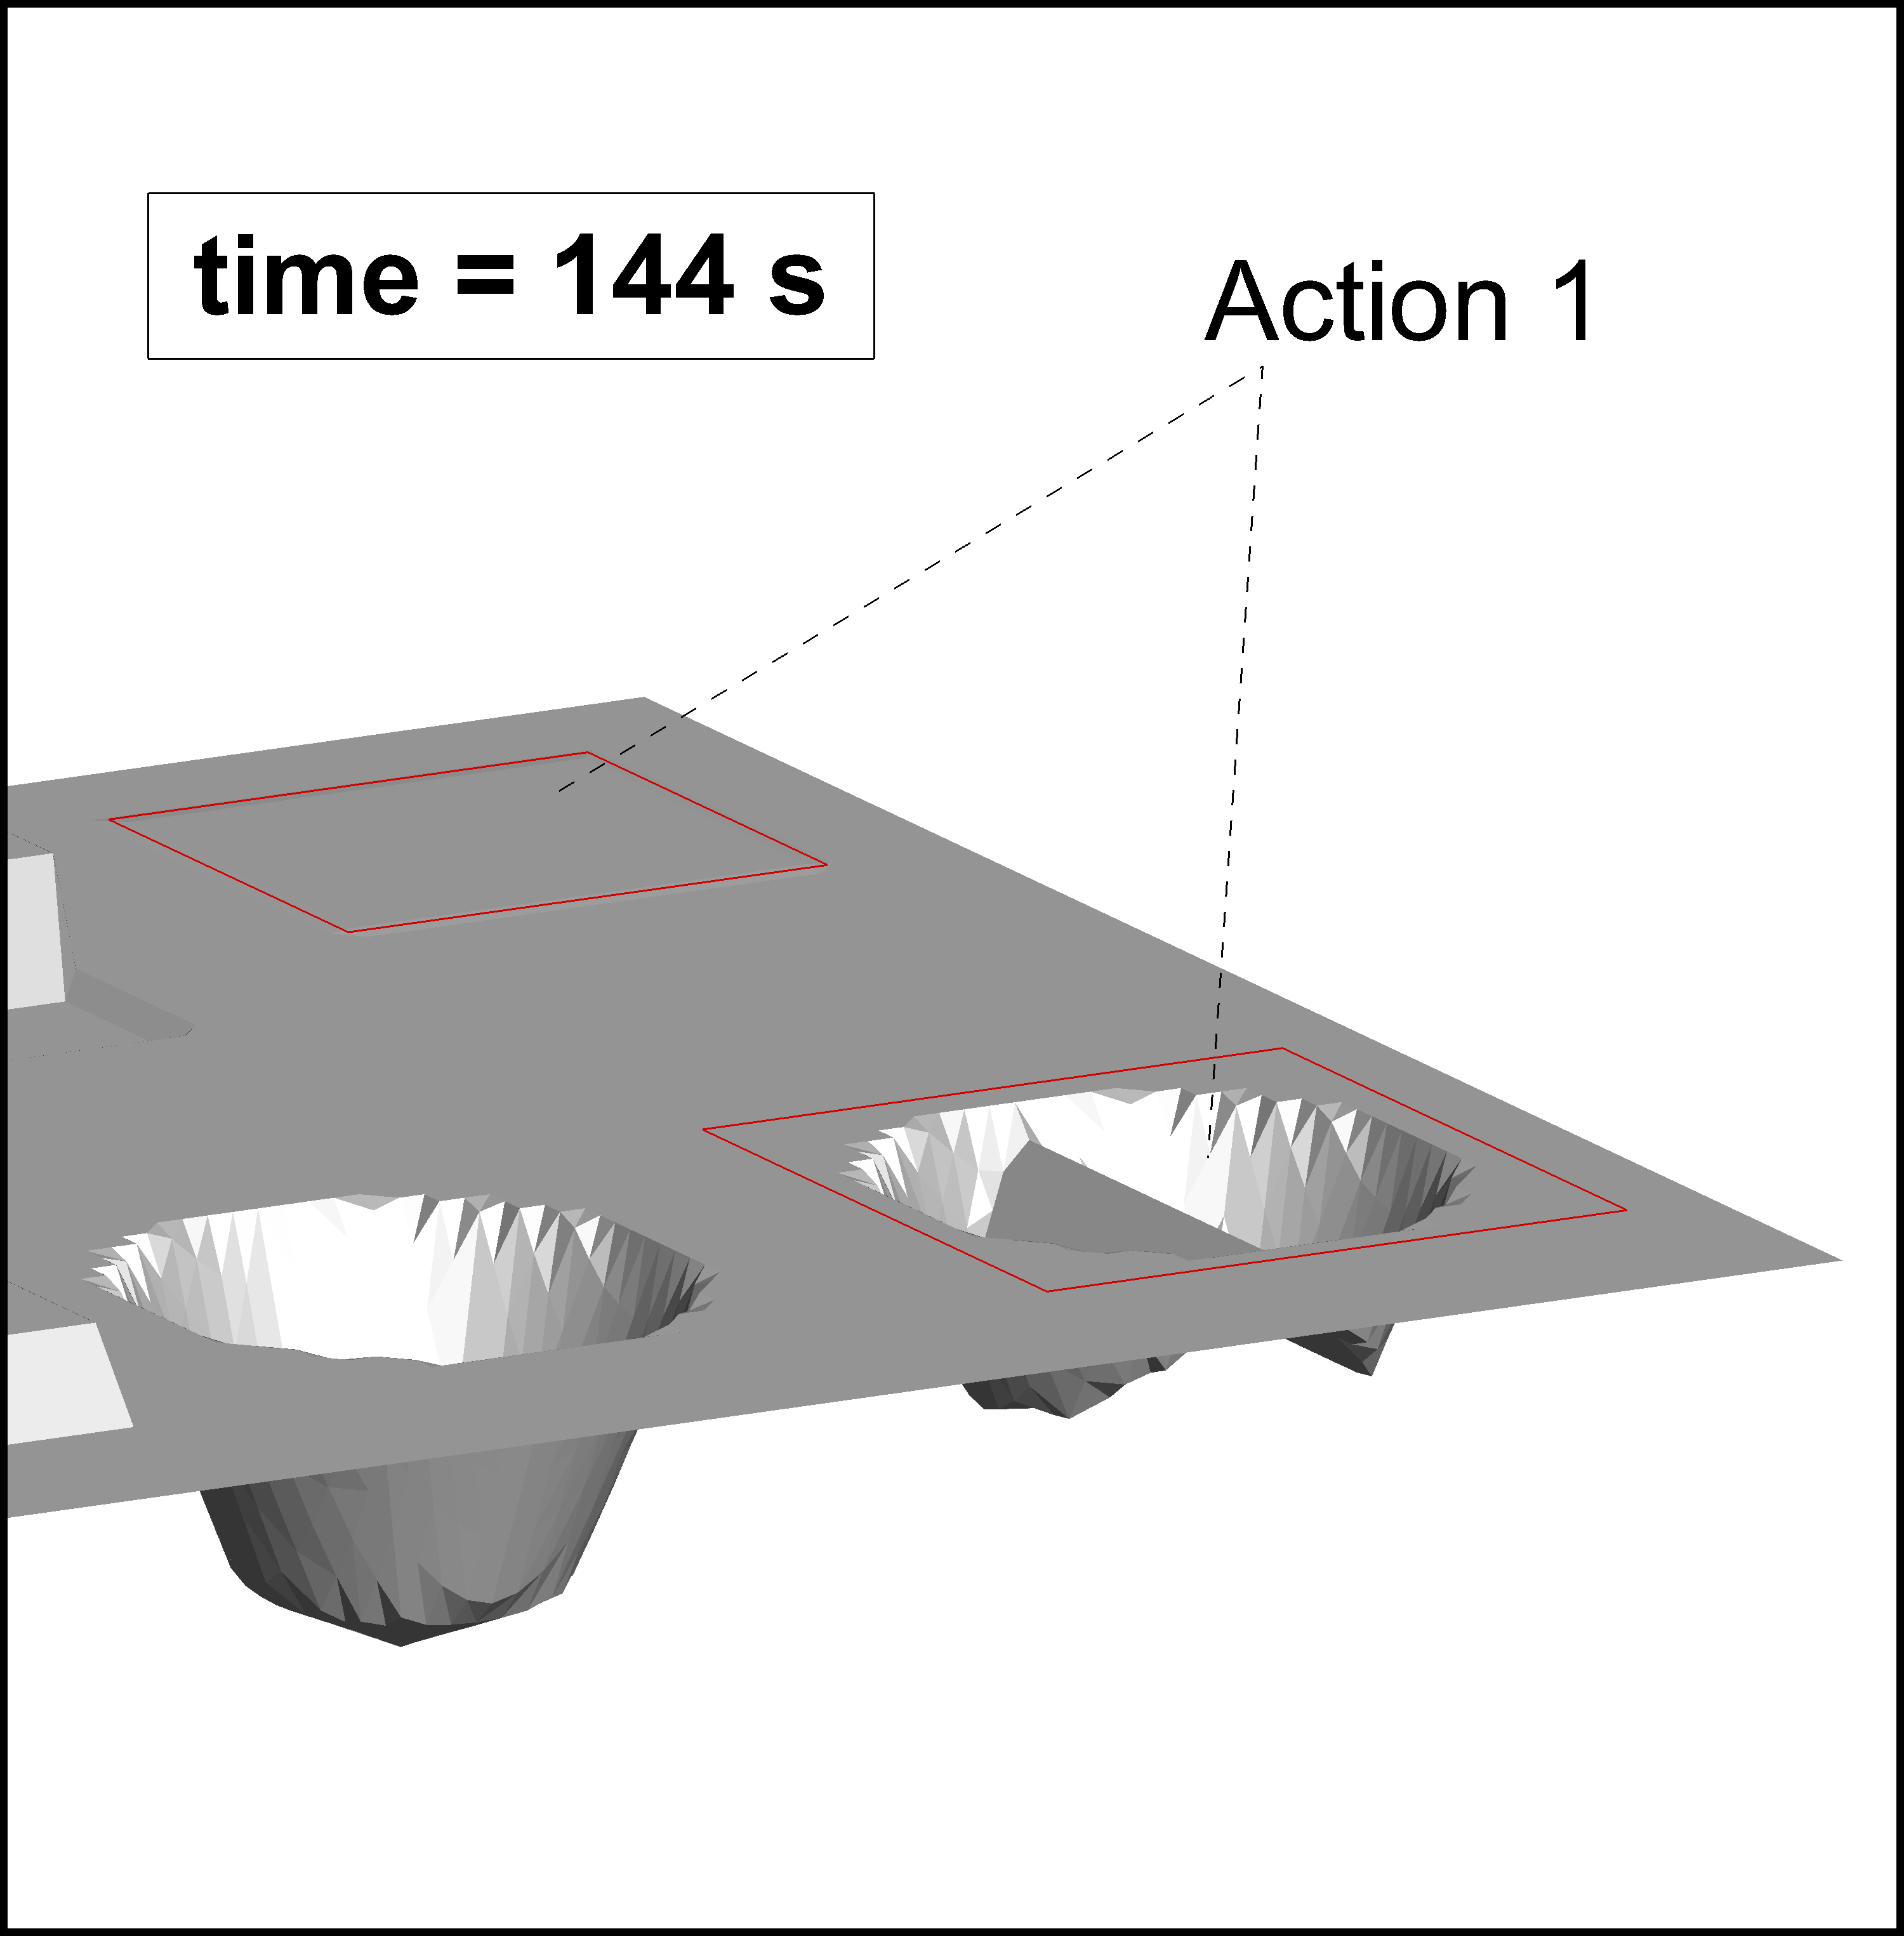
\includegraphics[width=0.45\textwidth]{img/Bild_Act1_144s.png}}
  \caption{Changes of the bottom while executing Action-1}
  \label{Act1}
\end{figure}


% ******************************************************************
% ******************************************************************
% **                                                              **
% **                          Action-2                            **
% ******************************************************************
% ******************************************************************
\newpage
\subsection{Action-2: ActionType\, = \,Save\_water\_level , ReferenceLevel = WATERLVL1}
\label{ssec:E4Action2}
\textbf{Action-2 :}~~~\texttt{ActionType\,=\,Save\_water\_level}~~~At simulation time 00:00:45 the water
level which was calculated at the last time step will be stored to be used later as reference level.
It is assigned to \texttt{WATERLVL1}.
\\
\\
Excerpt from the action file where the Action-2 is defined:
\\ \hspace*{3mm} \texttt{\small{/================================================================}}
\\ \hspace*{3mm} \texttt{\small{ACTION}}
\\ \hspace*{3mm} \texttt{\small{~~ActionType~~~~~~=~Save\_water\_level}}
\\ \hspace*{3mm} \texttt{\small{~~ReferenceLevel~~=~~WATERLVL1}}
\\ \hspace*{3mm} \texttt{\small{~~TimeStart~~~~~~~=~~2000.01.01-00:00:45~~/~[yyyy.mm.dd-hh:mm:ss]}}
\\ \hspace*{3mm} \texttt{\small{ENDACTION}}
\\ \hspace*{3mm} \texttt{\small{/================================================================}}
\\
\\
\\
% ******************************************************************
% ******************************************************************
% **                                                              **
% **                          Action-3                            **
% ******************************************************************
% ******************************************************************
\subsection{Action-3: ActionType\, = \,Dig\_by\_time , ReferenceLevel = WATERLVL1}
\label{ssec:E4Action3}
\textbf{Action-3 :}~~~\texttt{ActionType\,=\,Dig\_by\_time}~~~In the flield \texttt{432\_ri\_middle\_low} a
volume of 100\,m$^3$ will be dredged during the next 100\,s.
The time slot begins at simulation time 00:01:02 (hh:mm:ss). Because there is no setting for
the dump rate, the dumping into the flield \texttt{422\_le\_middle\_low} will be executed completely while dredging.
\\Because of the setting \texttt{DumpPlanar=TRUE} and \texttt{ReferenceLevel=WATERLVL1}, the
water level is used as reference level. The water level was saved beforehand in Action-2.
The bottom, where the dumping happened is shaped nearly flat (fig.\,\ref{Act3}d) referring to the shape of
the water level. \\
\\
Excerpt from the action file where the Action-3 is defined:
\\ \hspace*{3mm} \texttt{\small{/================================================================}}
\\ \hspace*{3mm} \texttt{\small{ACTION}}
\\ \hspace*{3mm} \texttt{\small{~~ActionType~~~~~~=~Dig\_by\_time}}
\\ \hspace*{3mm} \texttt{\small{~~ReferenceLevel~~=~~WATERLVL1}}
\\ \hspace*{3mm} \texttt{\small{~~TimeStart~~~~~~~=~~2000.01.01-00:01:02~~/~[yyyy.mm.dd-hh:mm:ss]}}
\\ \hspace*{3mm} \texttt{\small{~~TimeEnd~~~~~~~~~=~~2000.01.01-00:02:42~~/~[yyyy.mm.dd-hh:mm:ss]}}
\\ \hspace*{3mm}
\\ \hspace*{3mm} \texttt{\small{~~FieldDig~~~~~~~~=~~432\_ri\_middle\_low}}
\\ \hspace*{3mm} \texttt{\small{~~DigVolume~~~~~~~=~~100.0~~~~~~~~~~~~~~~~/~[m\textasciicircum3]}}
\\ \hspace*{3mm}
\\ \hspace*{3mm} \texttt{\small{~~FieldDump~~~~~~~=~~422\_le\_middle\_low}}
\\ \hspace*{3mm} \texttt{\small{~~DumpPlanar~~~~~~=~~TRUE}}
\\ \hspace*{3mm} \texttt{\small{ENDACTION}}
\\ \hspace*{3mm} \texttt{\small{/================================================================}}

\begin{figure}[H]
  \centering
    \subfloat[]                    {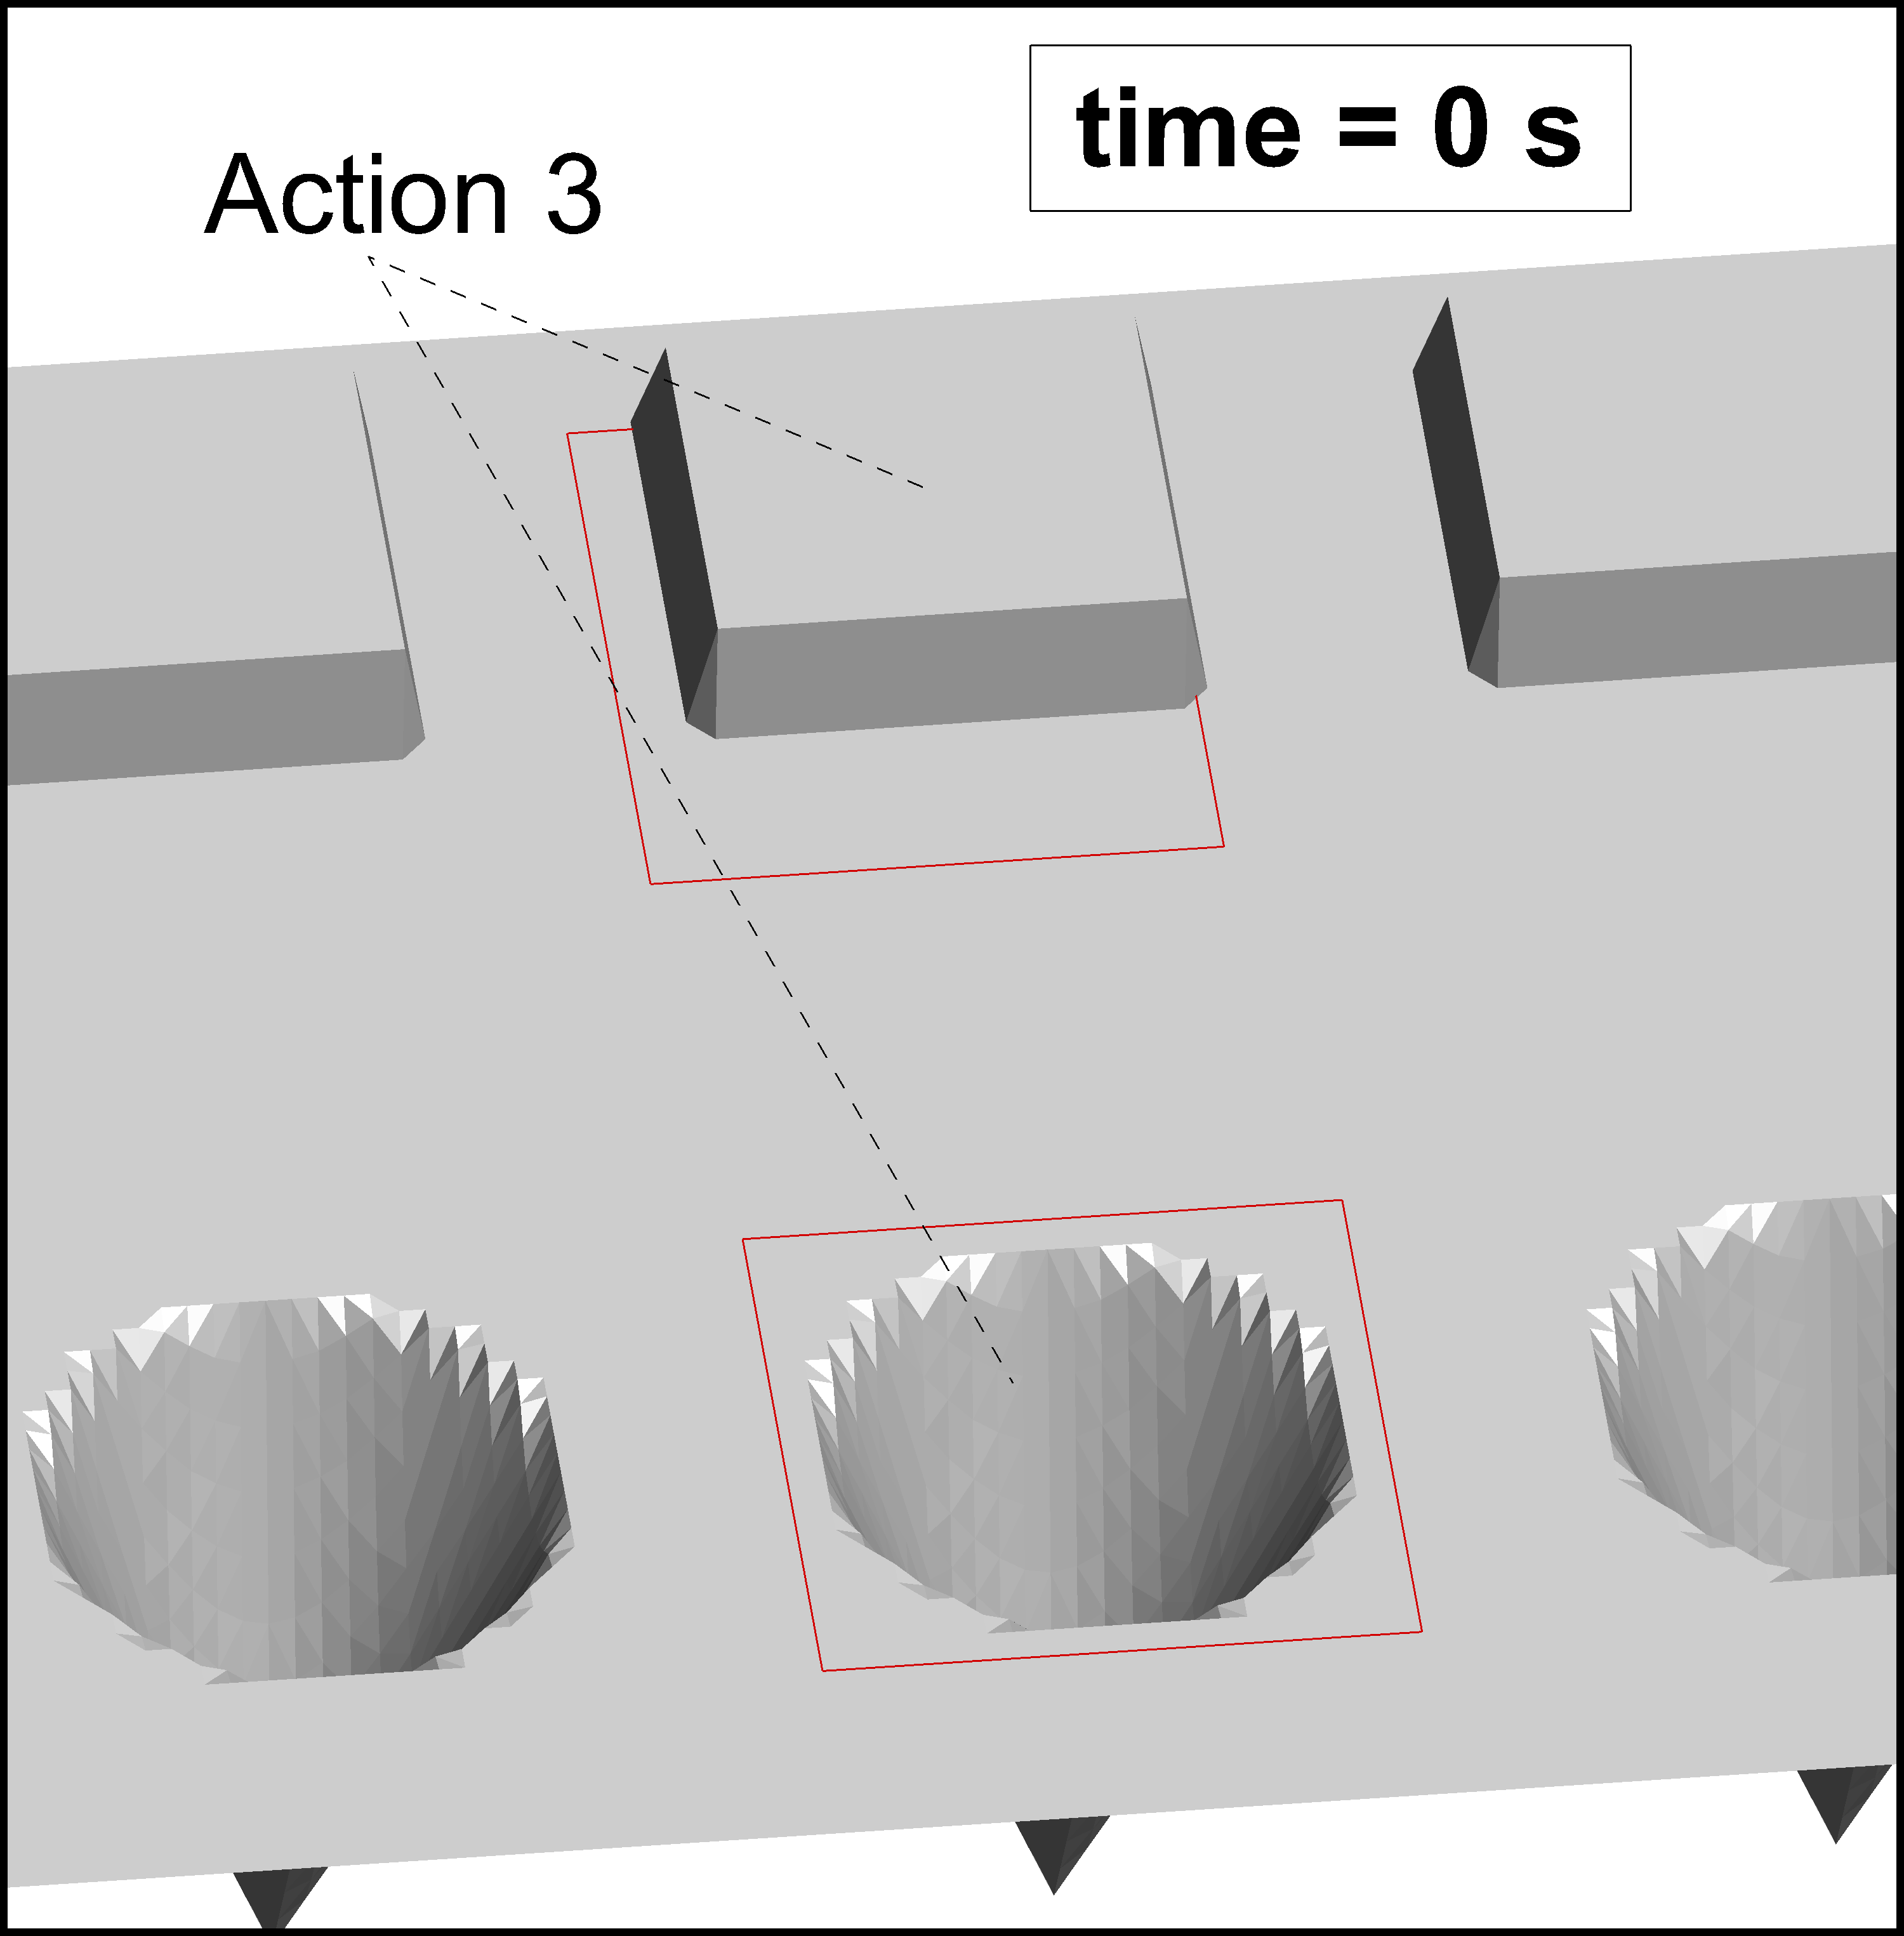
\includegraphics[width=0.45\textwidth]{img/Bild_Act3_000s.png}}\qquad
    \subfloat[dredging and dumping
                      just started]{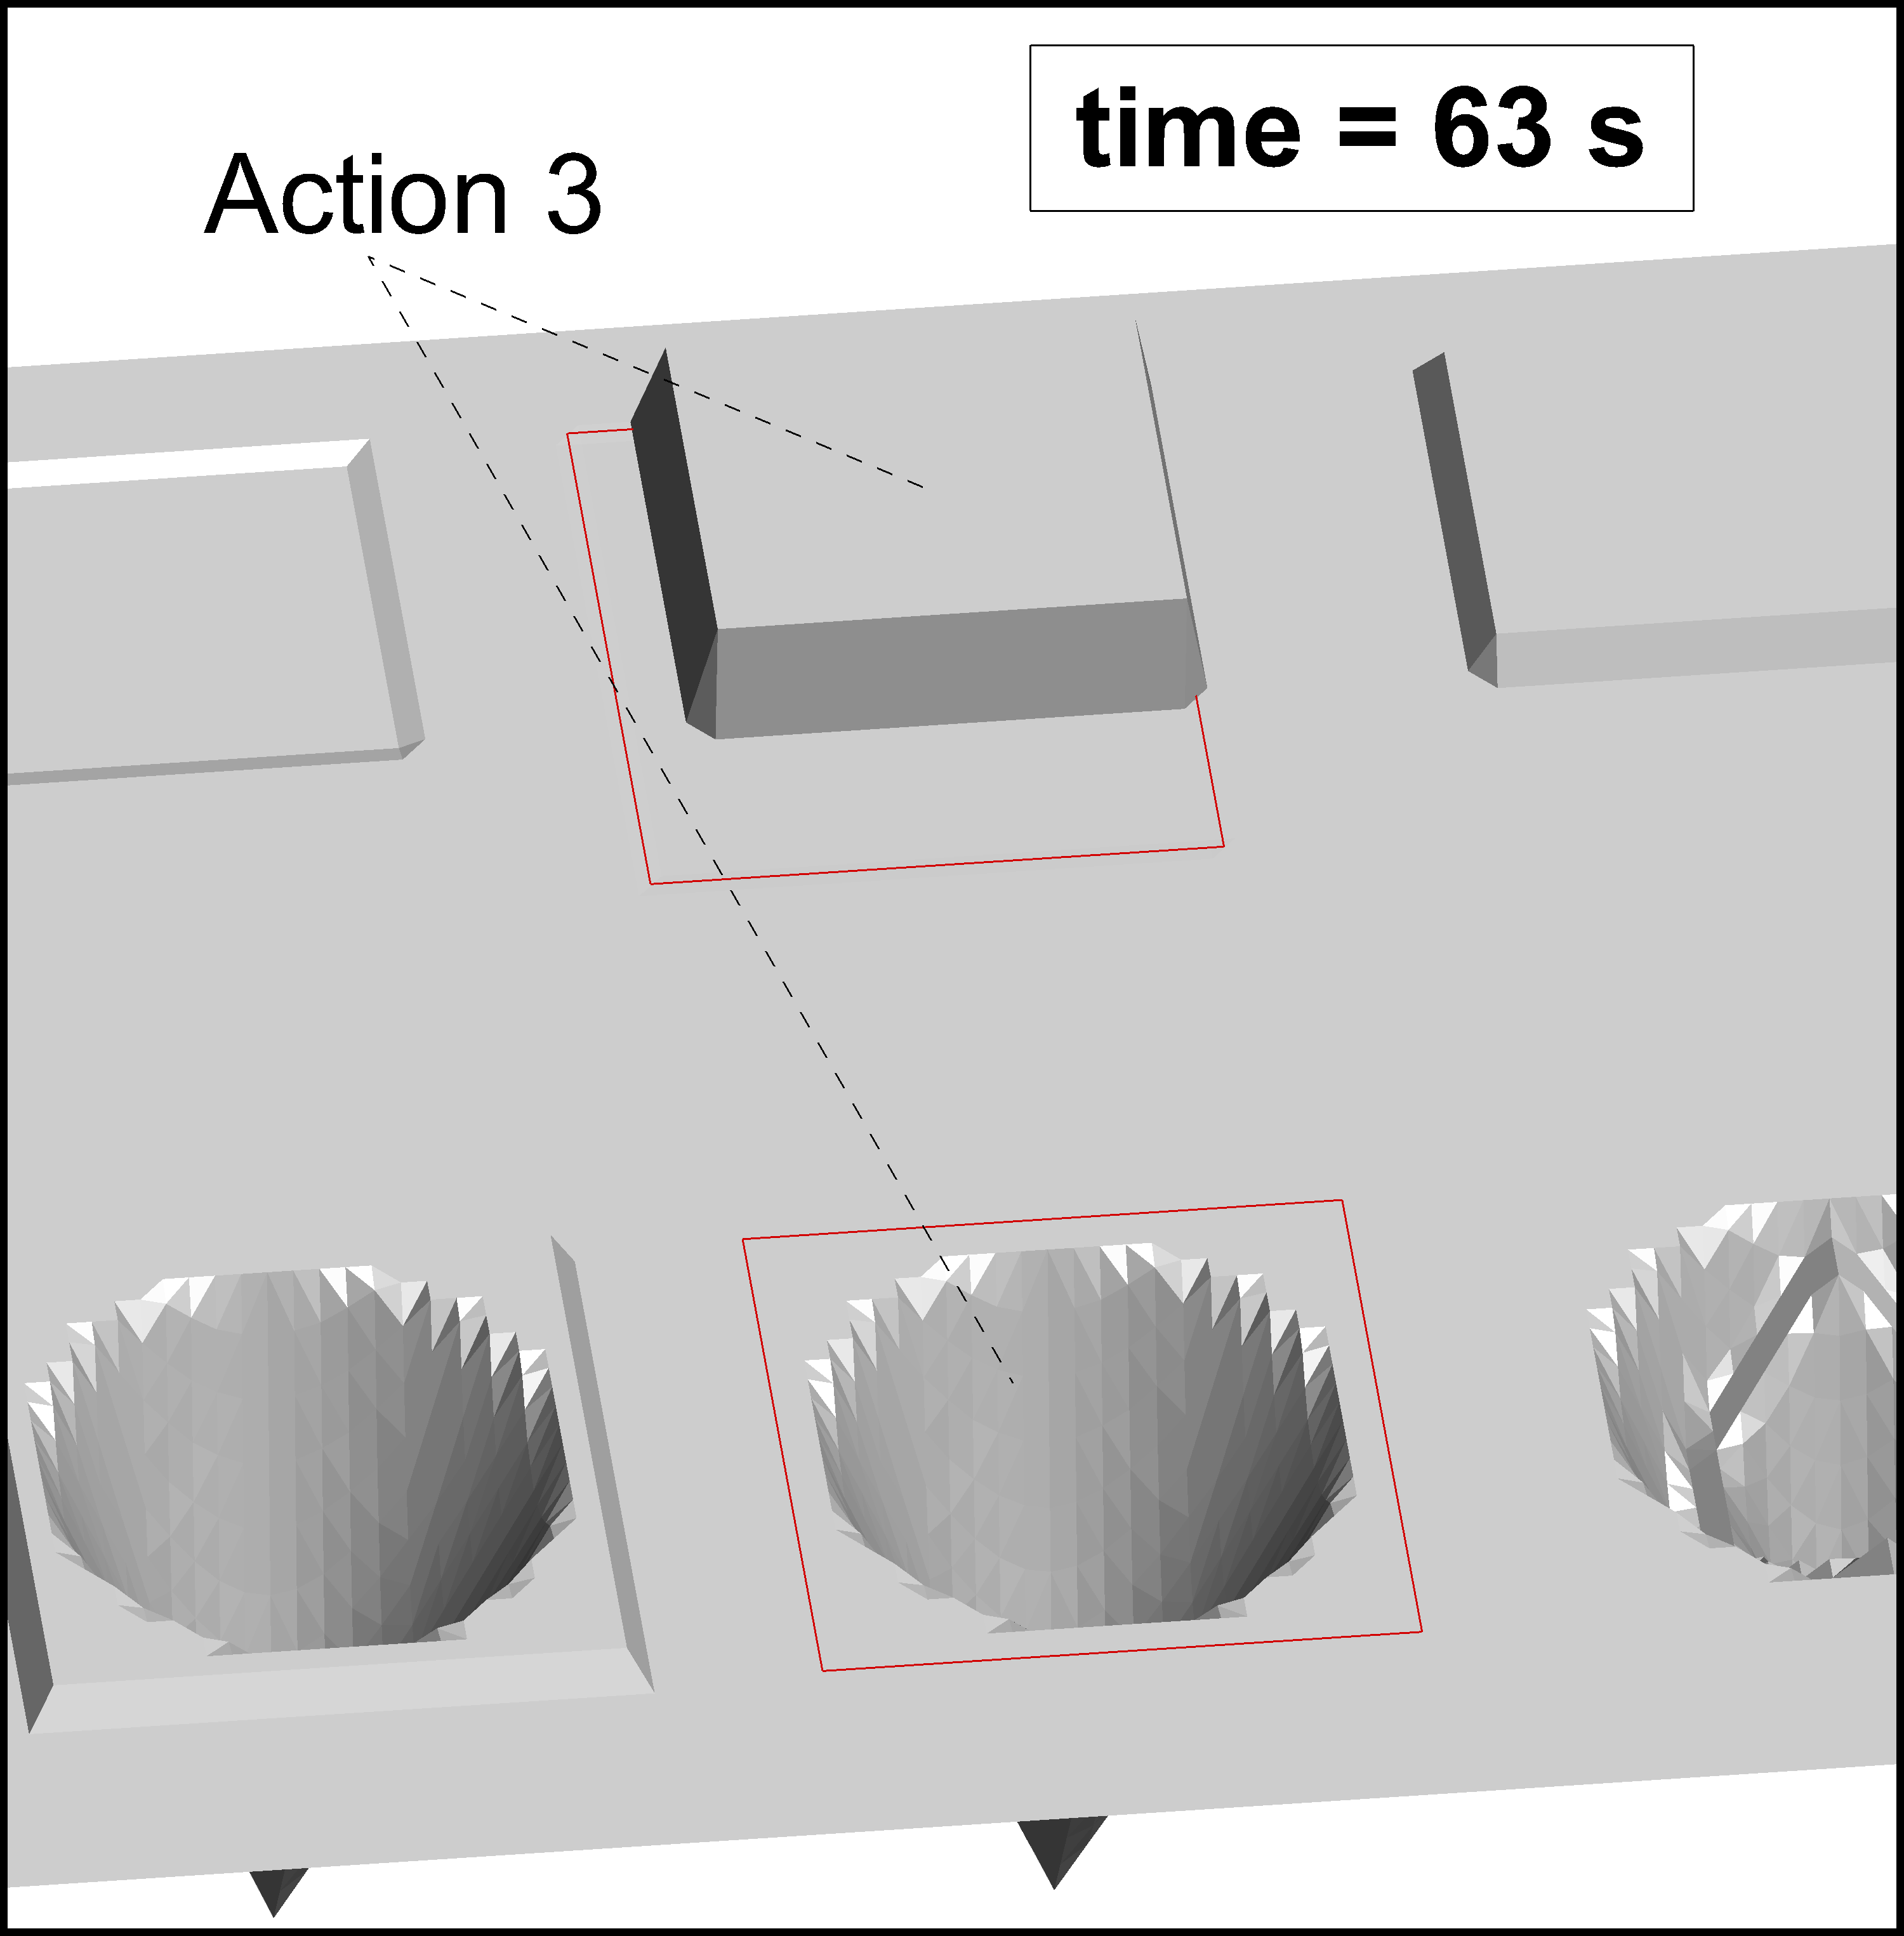
\includegraphics[width=0.45\textwidth]{img/Bild_Act3_063s.png}}\qquad
    \subfloat[dredging and dumping]{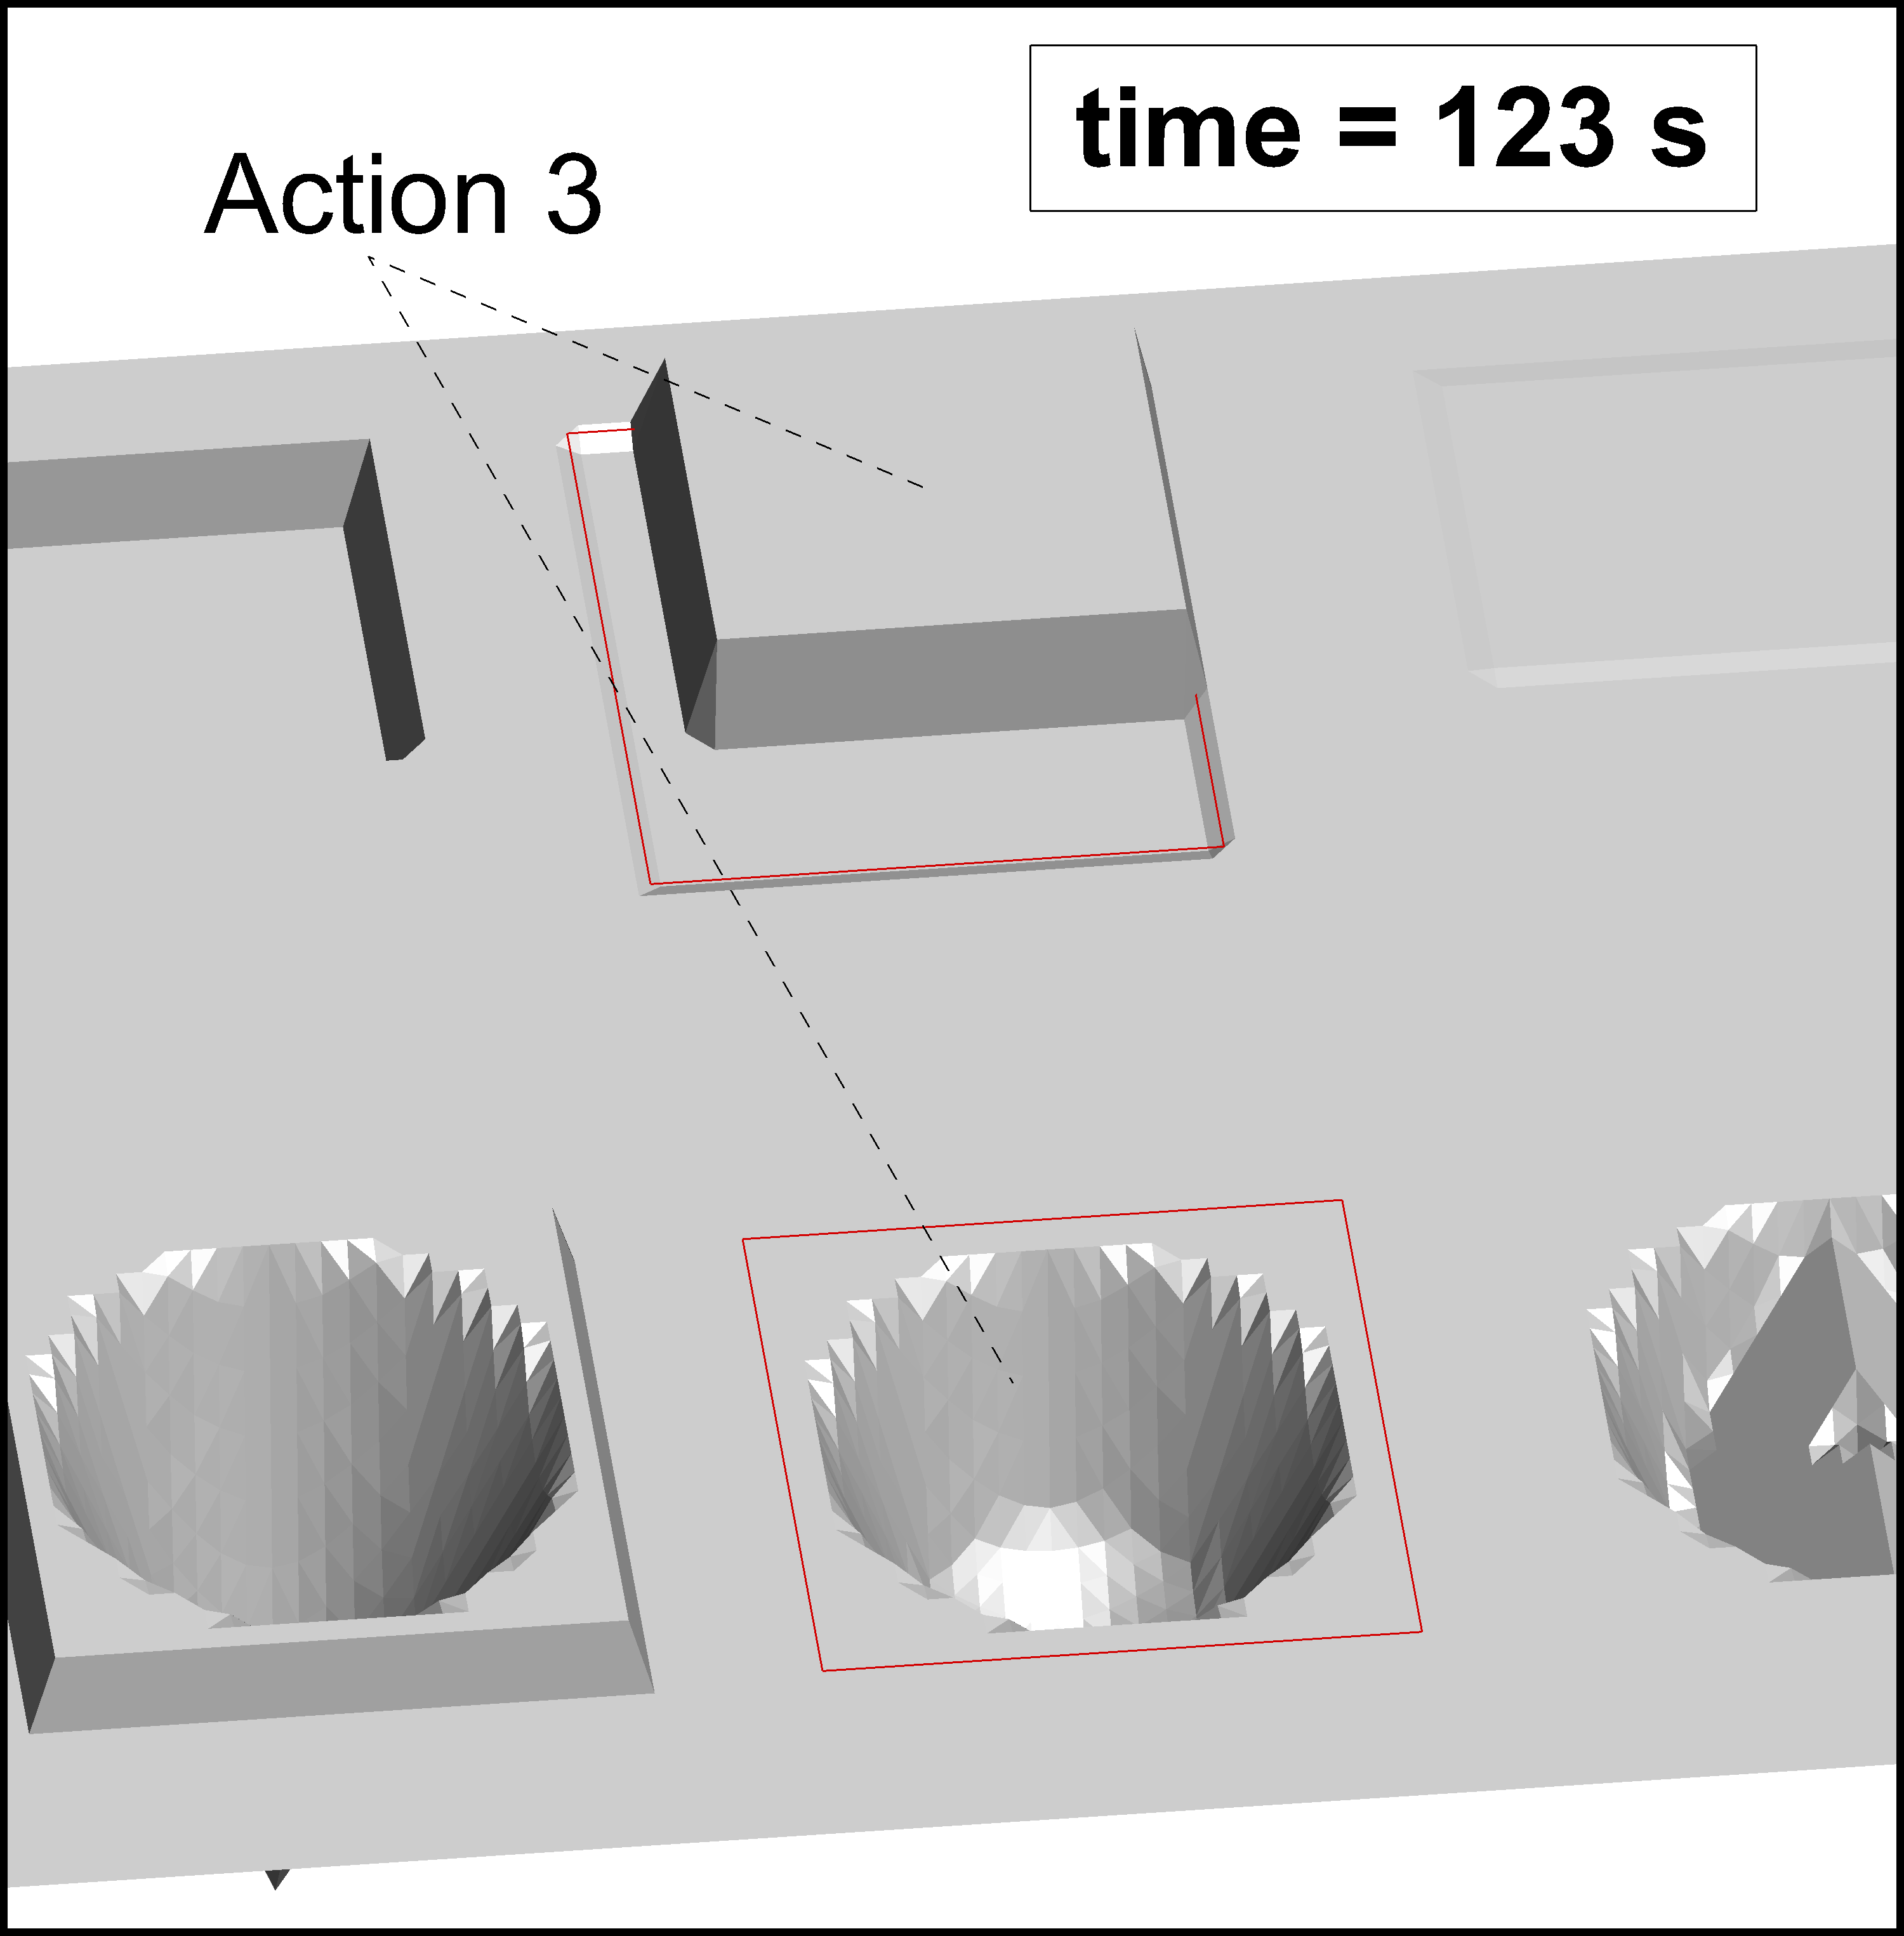
\includegraphics[width=0.45\textwidth]{img/Bild_Act3_123s.png}}\qquad
    \subfloat[dredging and dumping
                     just finished]{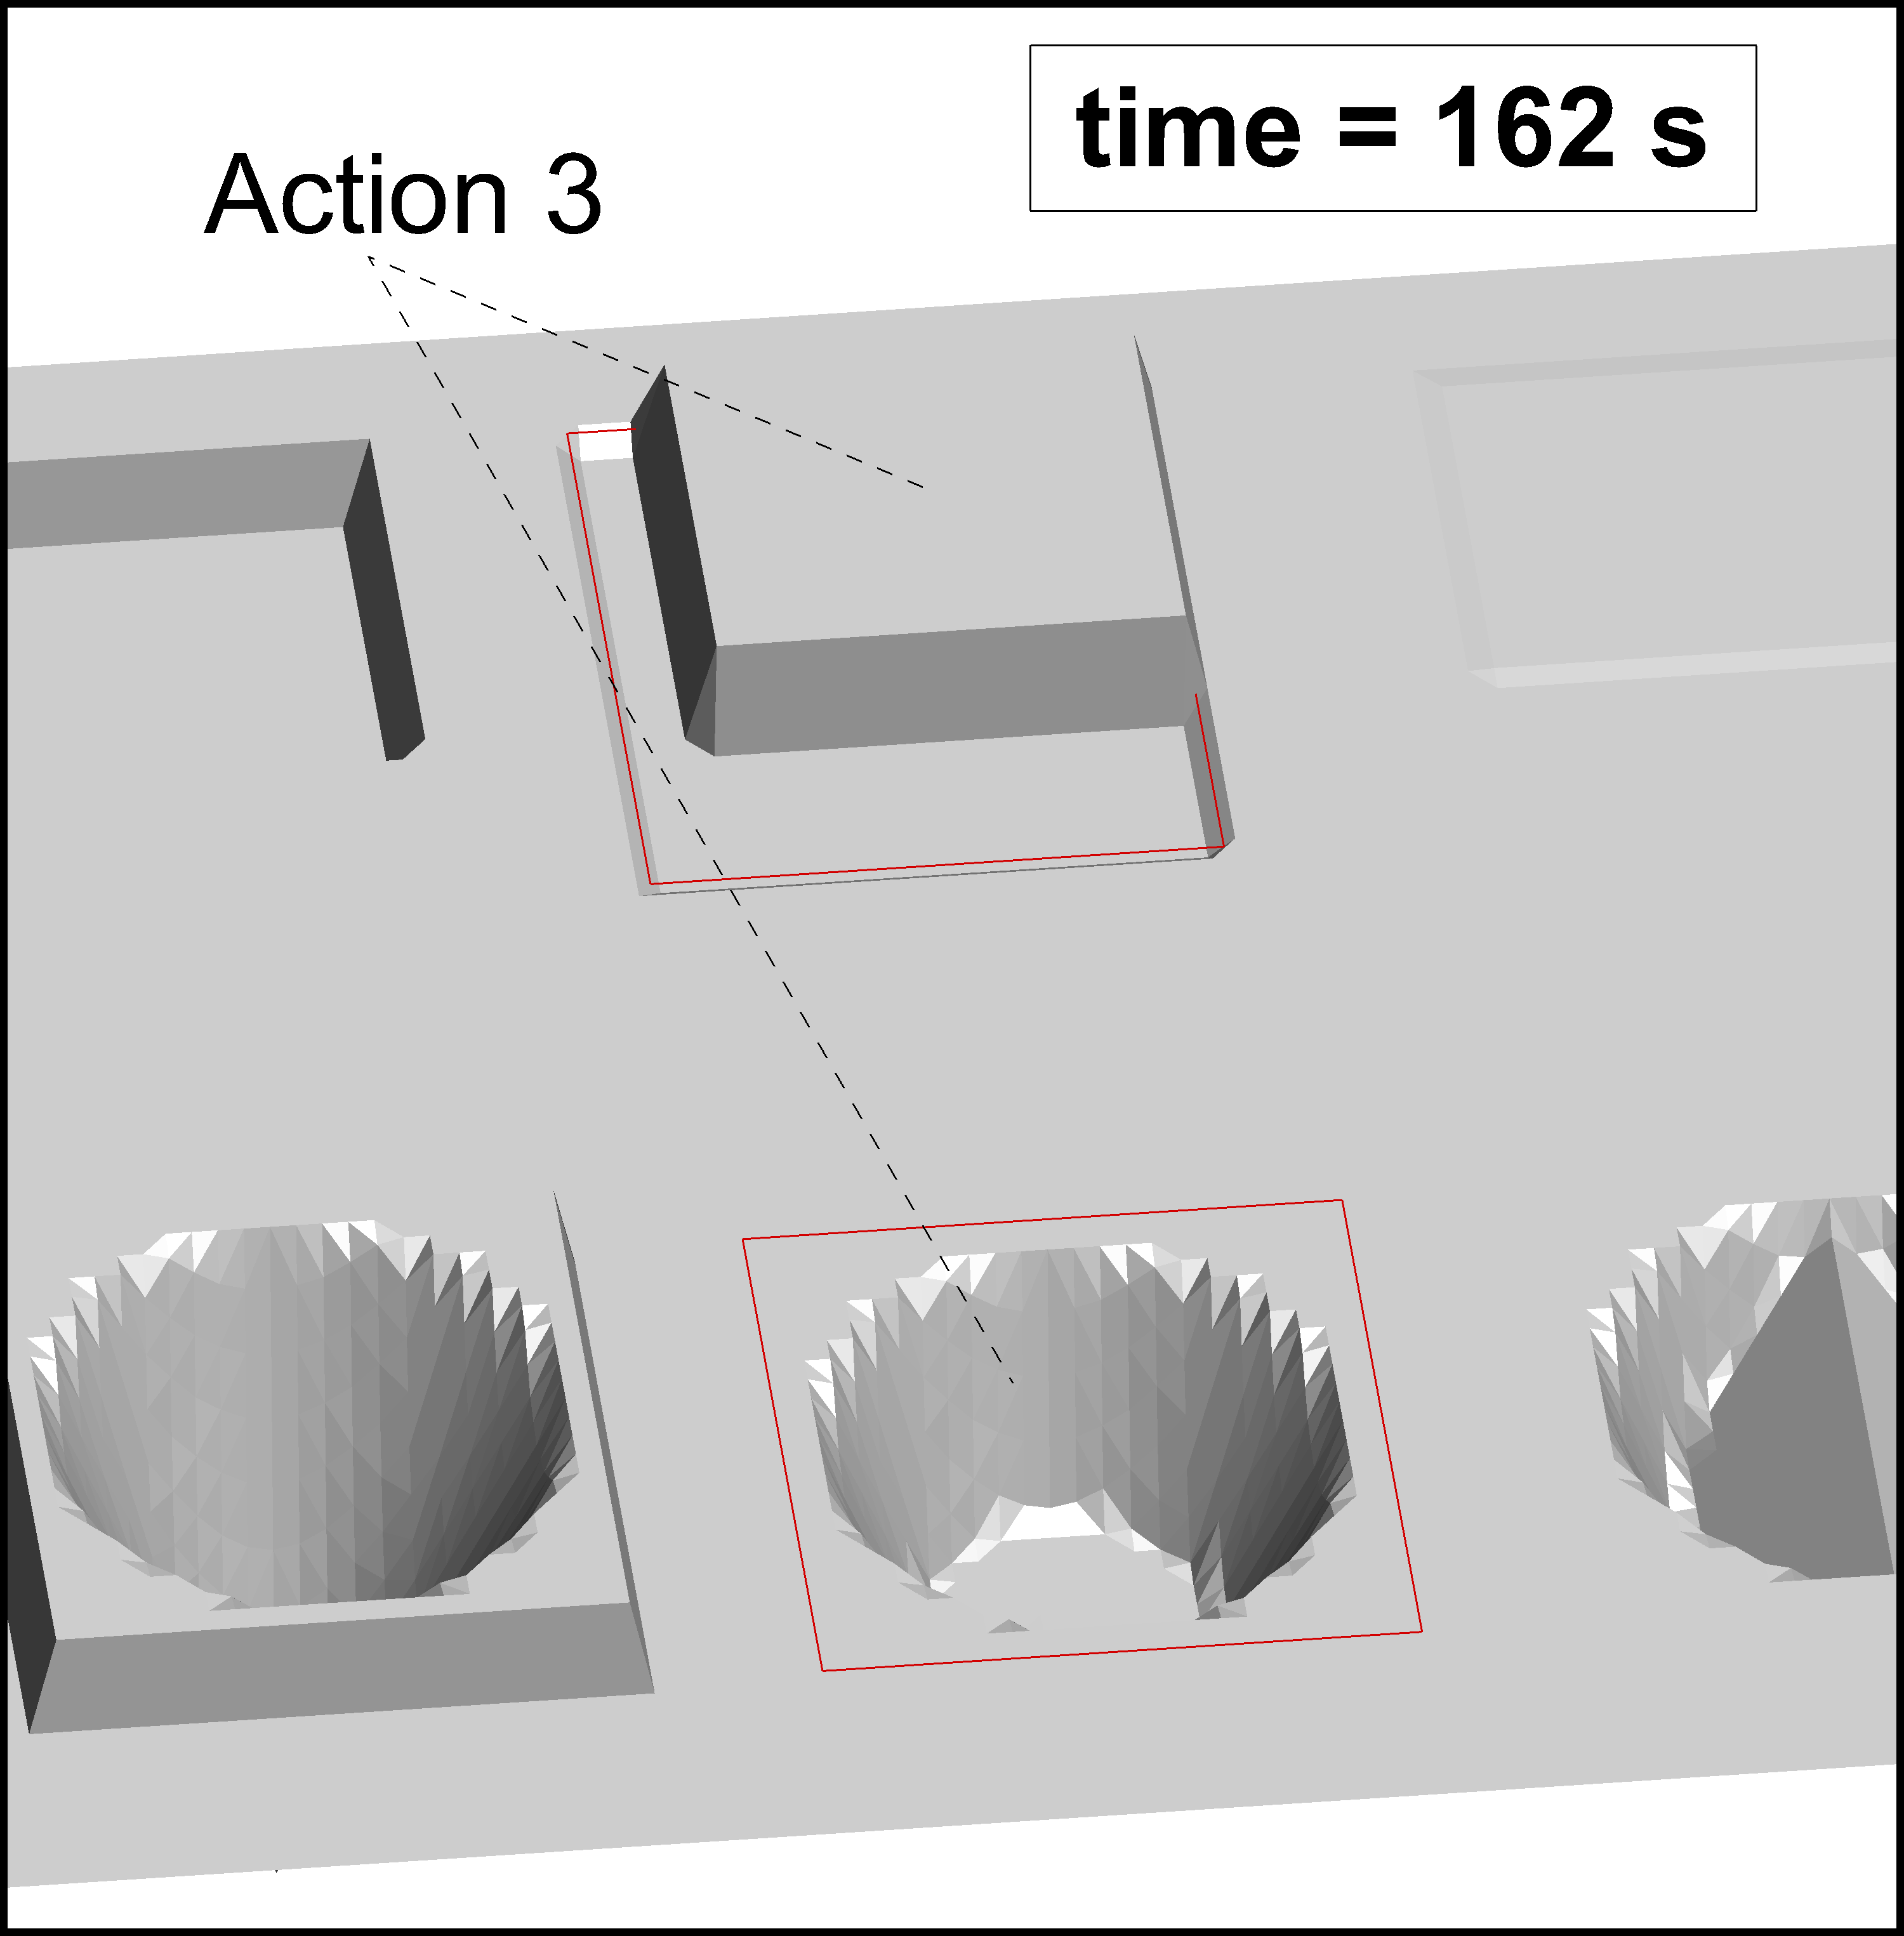
\includegraphics[width=0.45\textwidth]{img/Bild_Act3_162s.png}}
  \caption{Changes of the bottom while executing Action-3}
  \label{Act3}
\end{figure}

% ******************************************************************
% ******************************************************************
% **                                                              **
% **                          Action-4                            **
% ******************************************************************
% ******************************************************************
\newpage
\subsection{Action-4: ActionType\, = \,Dig\_by\_time , ReferenceLevel not used}
\label{ssec:E4Action4}
\textbf{Action-4 :}~~~\texttt{ActionType\,=\,Dig\_by\_time}~~~In the flield \texttt{433\_ri\_middle\_high},
beginning at simulation time 00:00:02, a volume of 529\,m$^3$ will be dredged during the next 100\,s.
Every node in the field will be lowered by 1.74\,m (fig.\,\ref{Act4}c).
Simultaneously the dredged material will be dumped into the field \texttt{423\_le\_middle\_high\_down}.
Because of the setting \texttt{DumpPlanar=FALSE}, a reference level is not used.
As a result, every node in the dump field will be elevated by the same value, in this case 1.0\,m (fig.\,\ref{Act4}c).\\
Due to the setting \texttt{DumpRate=0.005}, the dumping is slow and
it takes 200\,s to dump all of the dredged volume (fig.\,\ref{Act4}d).
\\
\begin{figure}[H]
  \centering
    \subfloat[]                    {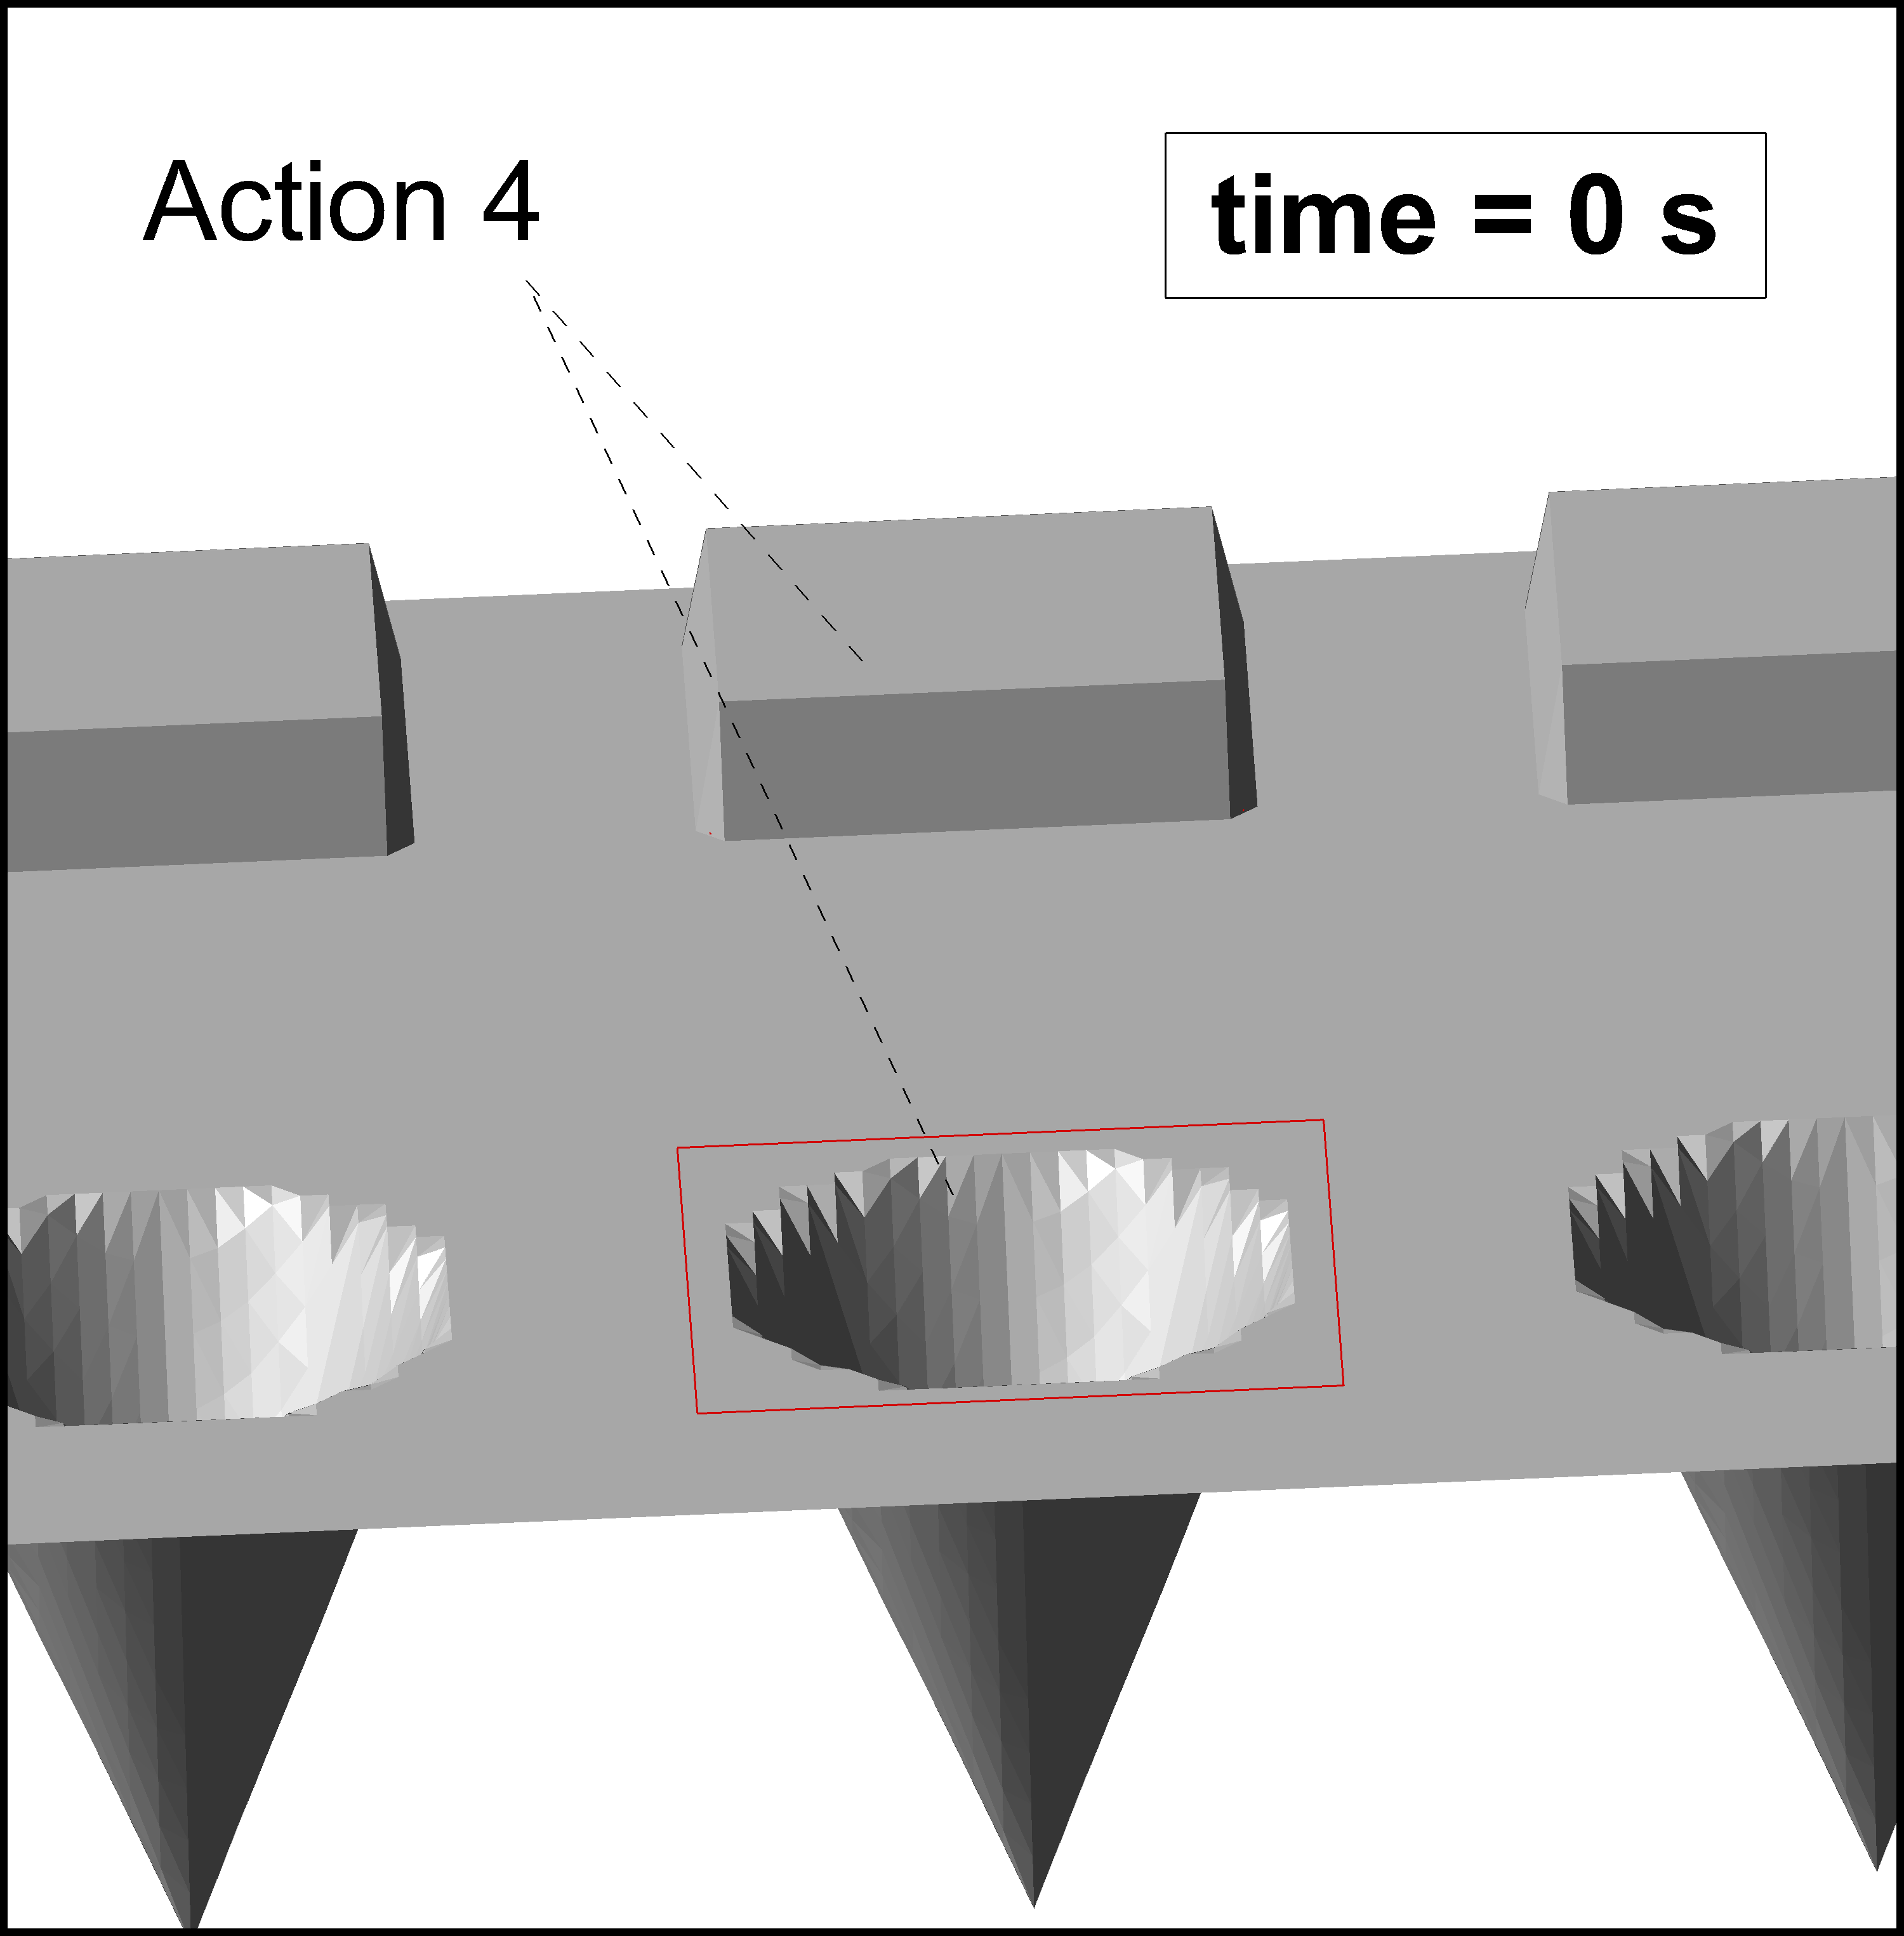
\includegraphics[width=0.45\textwidth]{img/Bild_Act4_000s.png}}\qquad
    \subfloat[dredging and dumping]{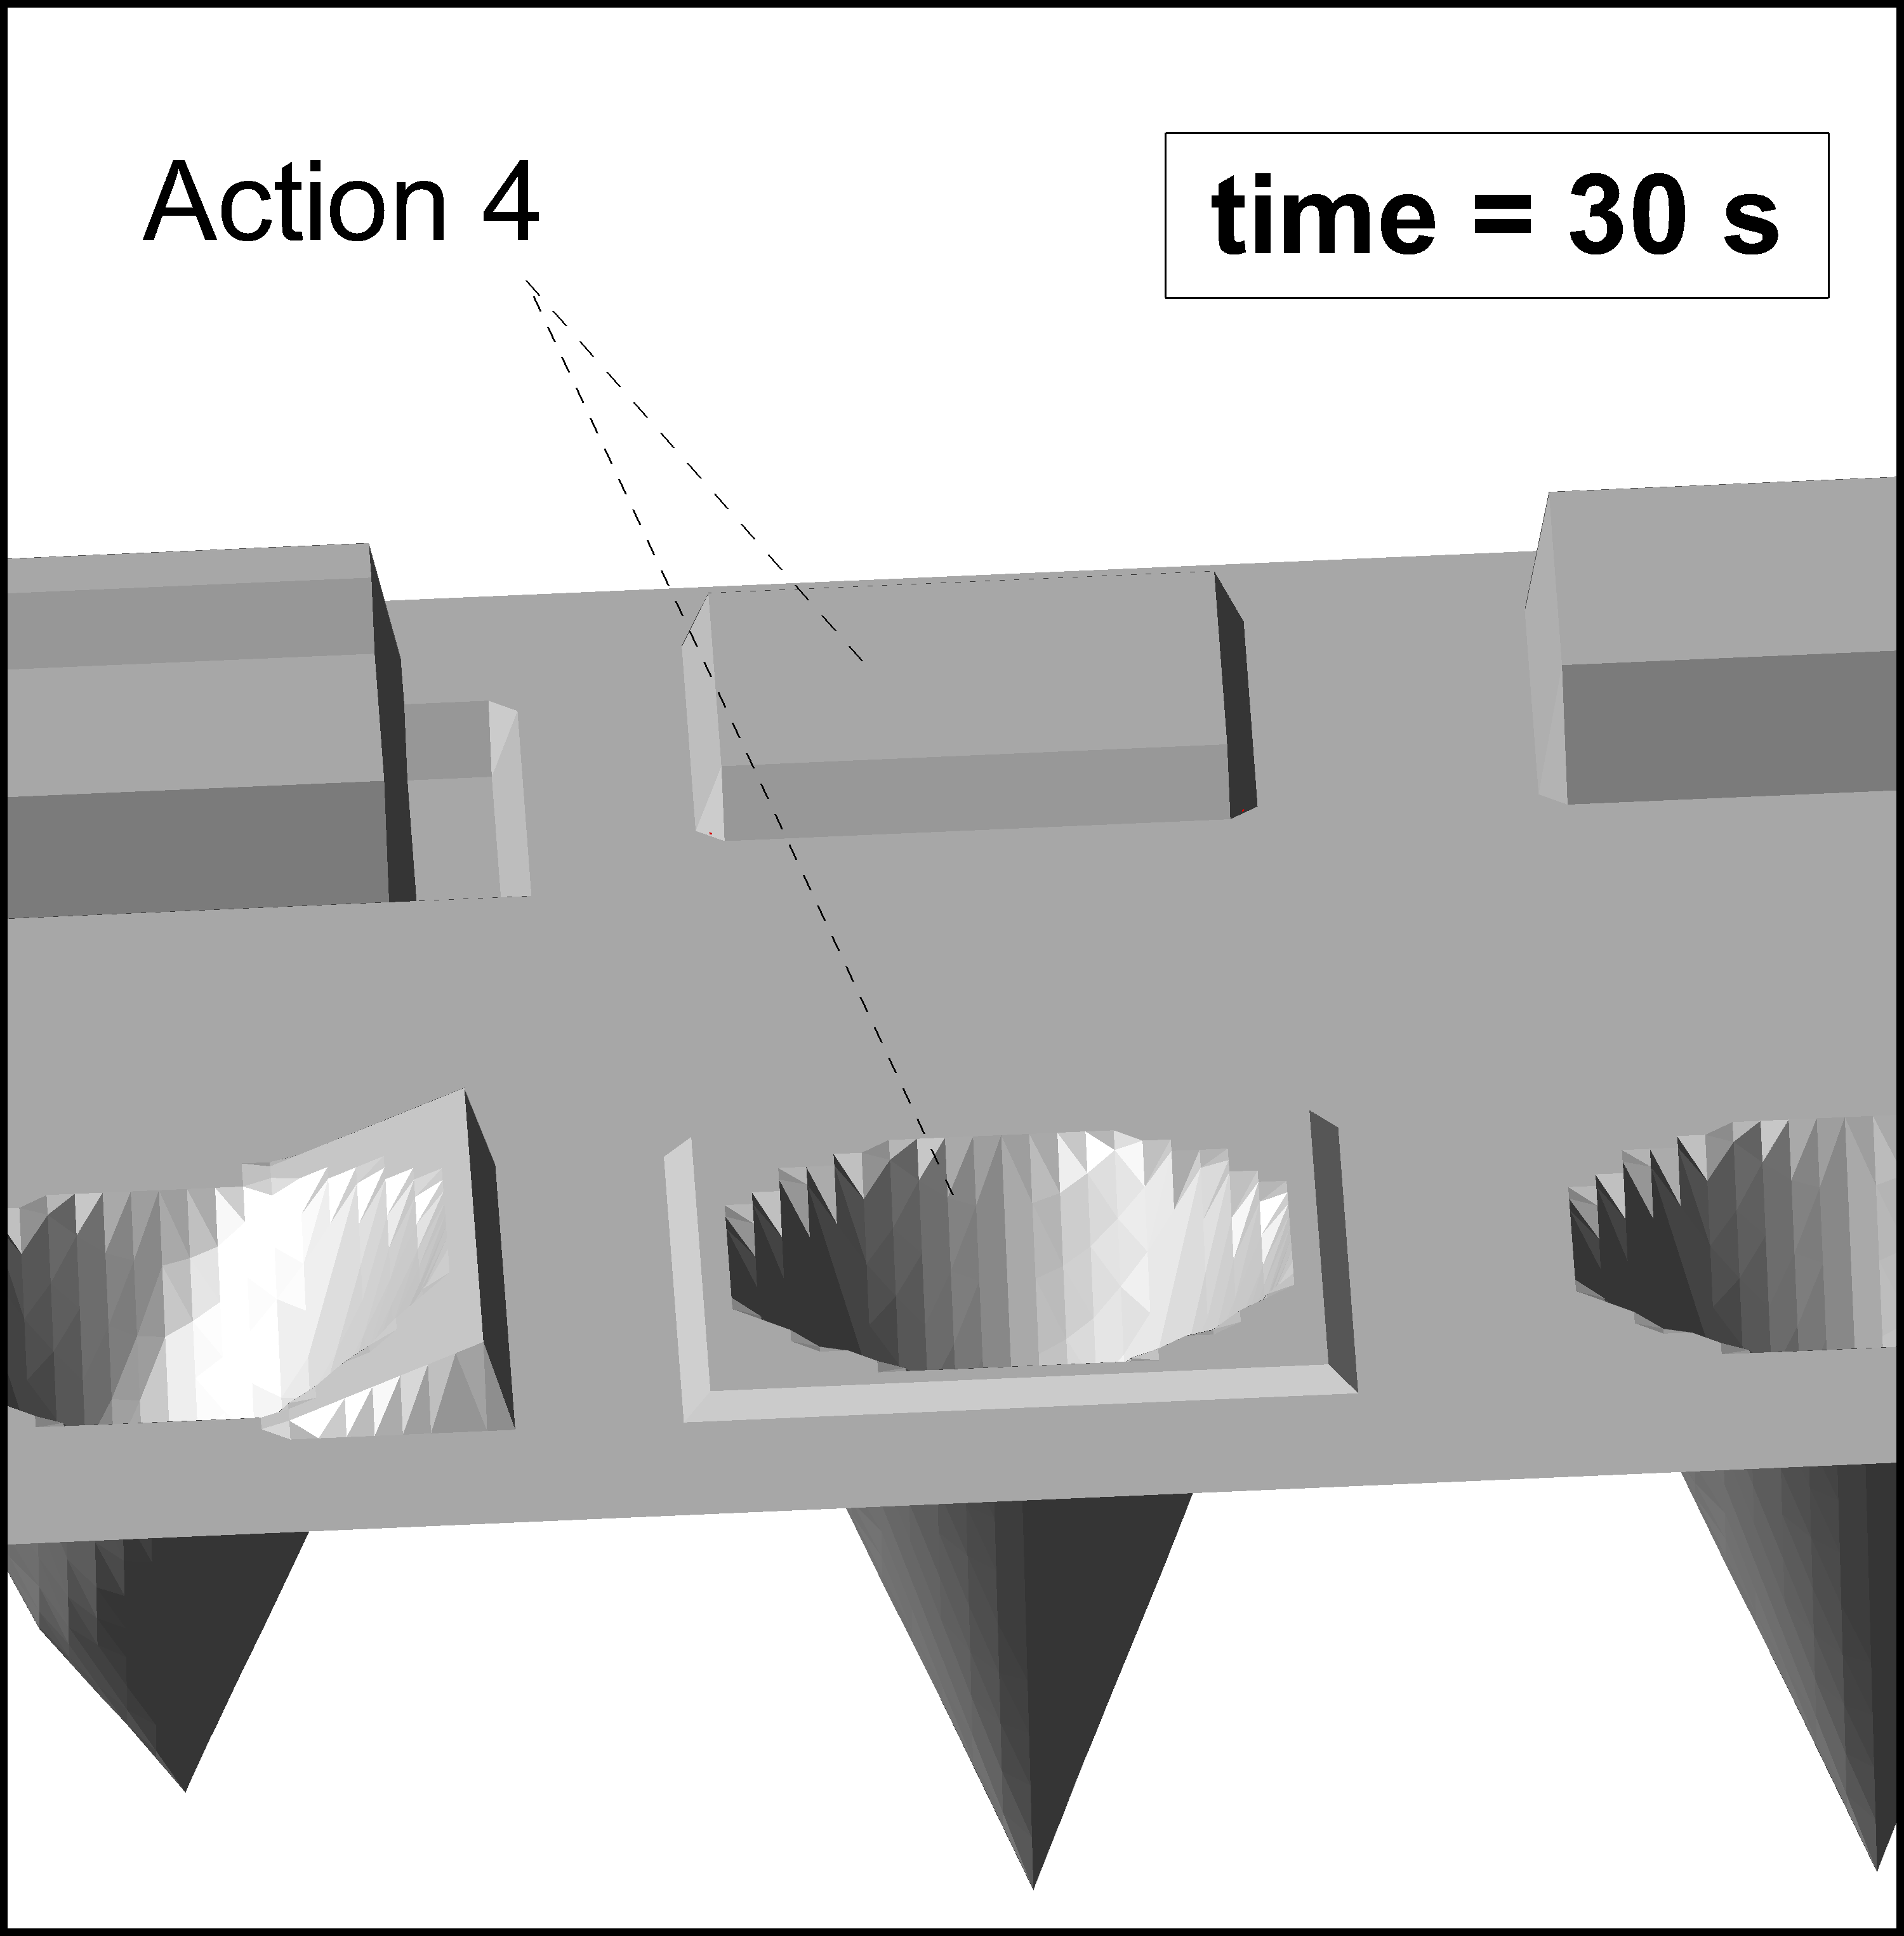
\includegraphics[width=0.45\textwidth]{img/Bild_Act4_030s.png}}\qquad
    \subfloat[dredging just finished,
                     still dumping]{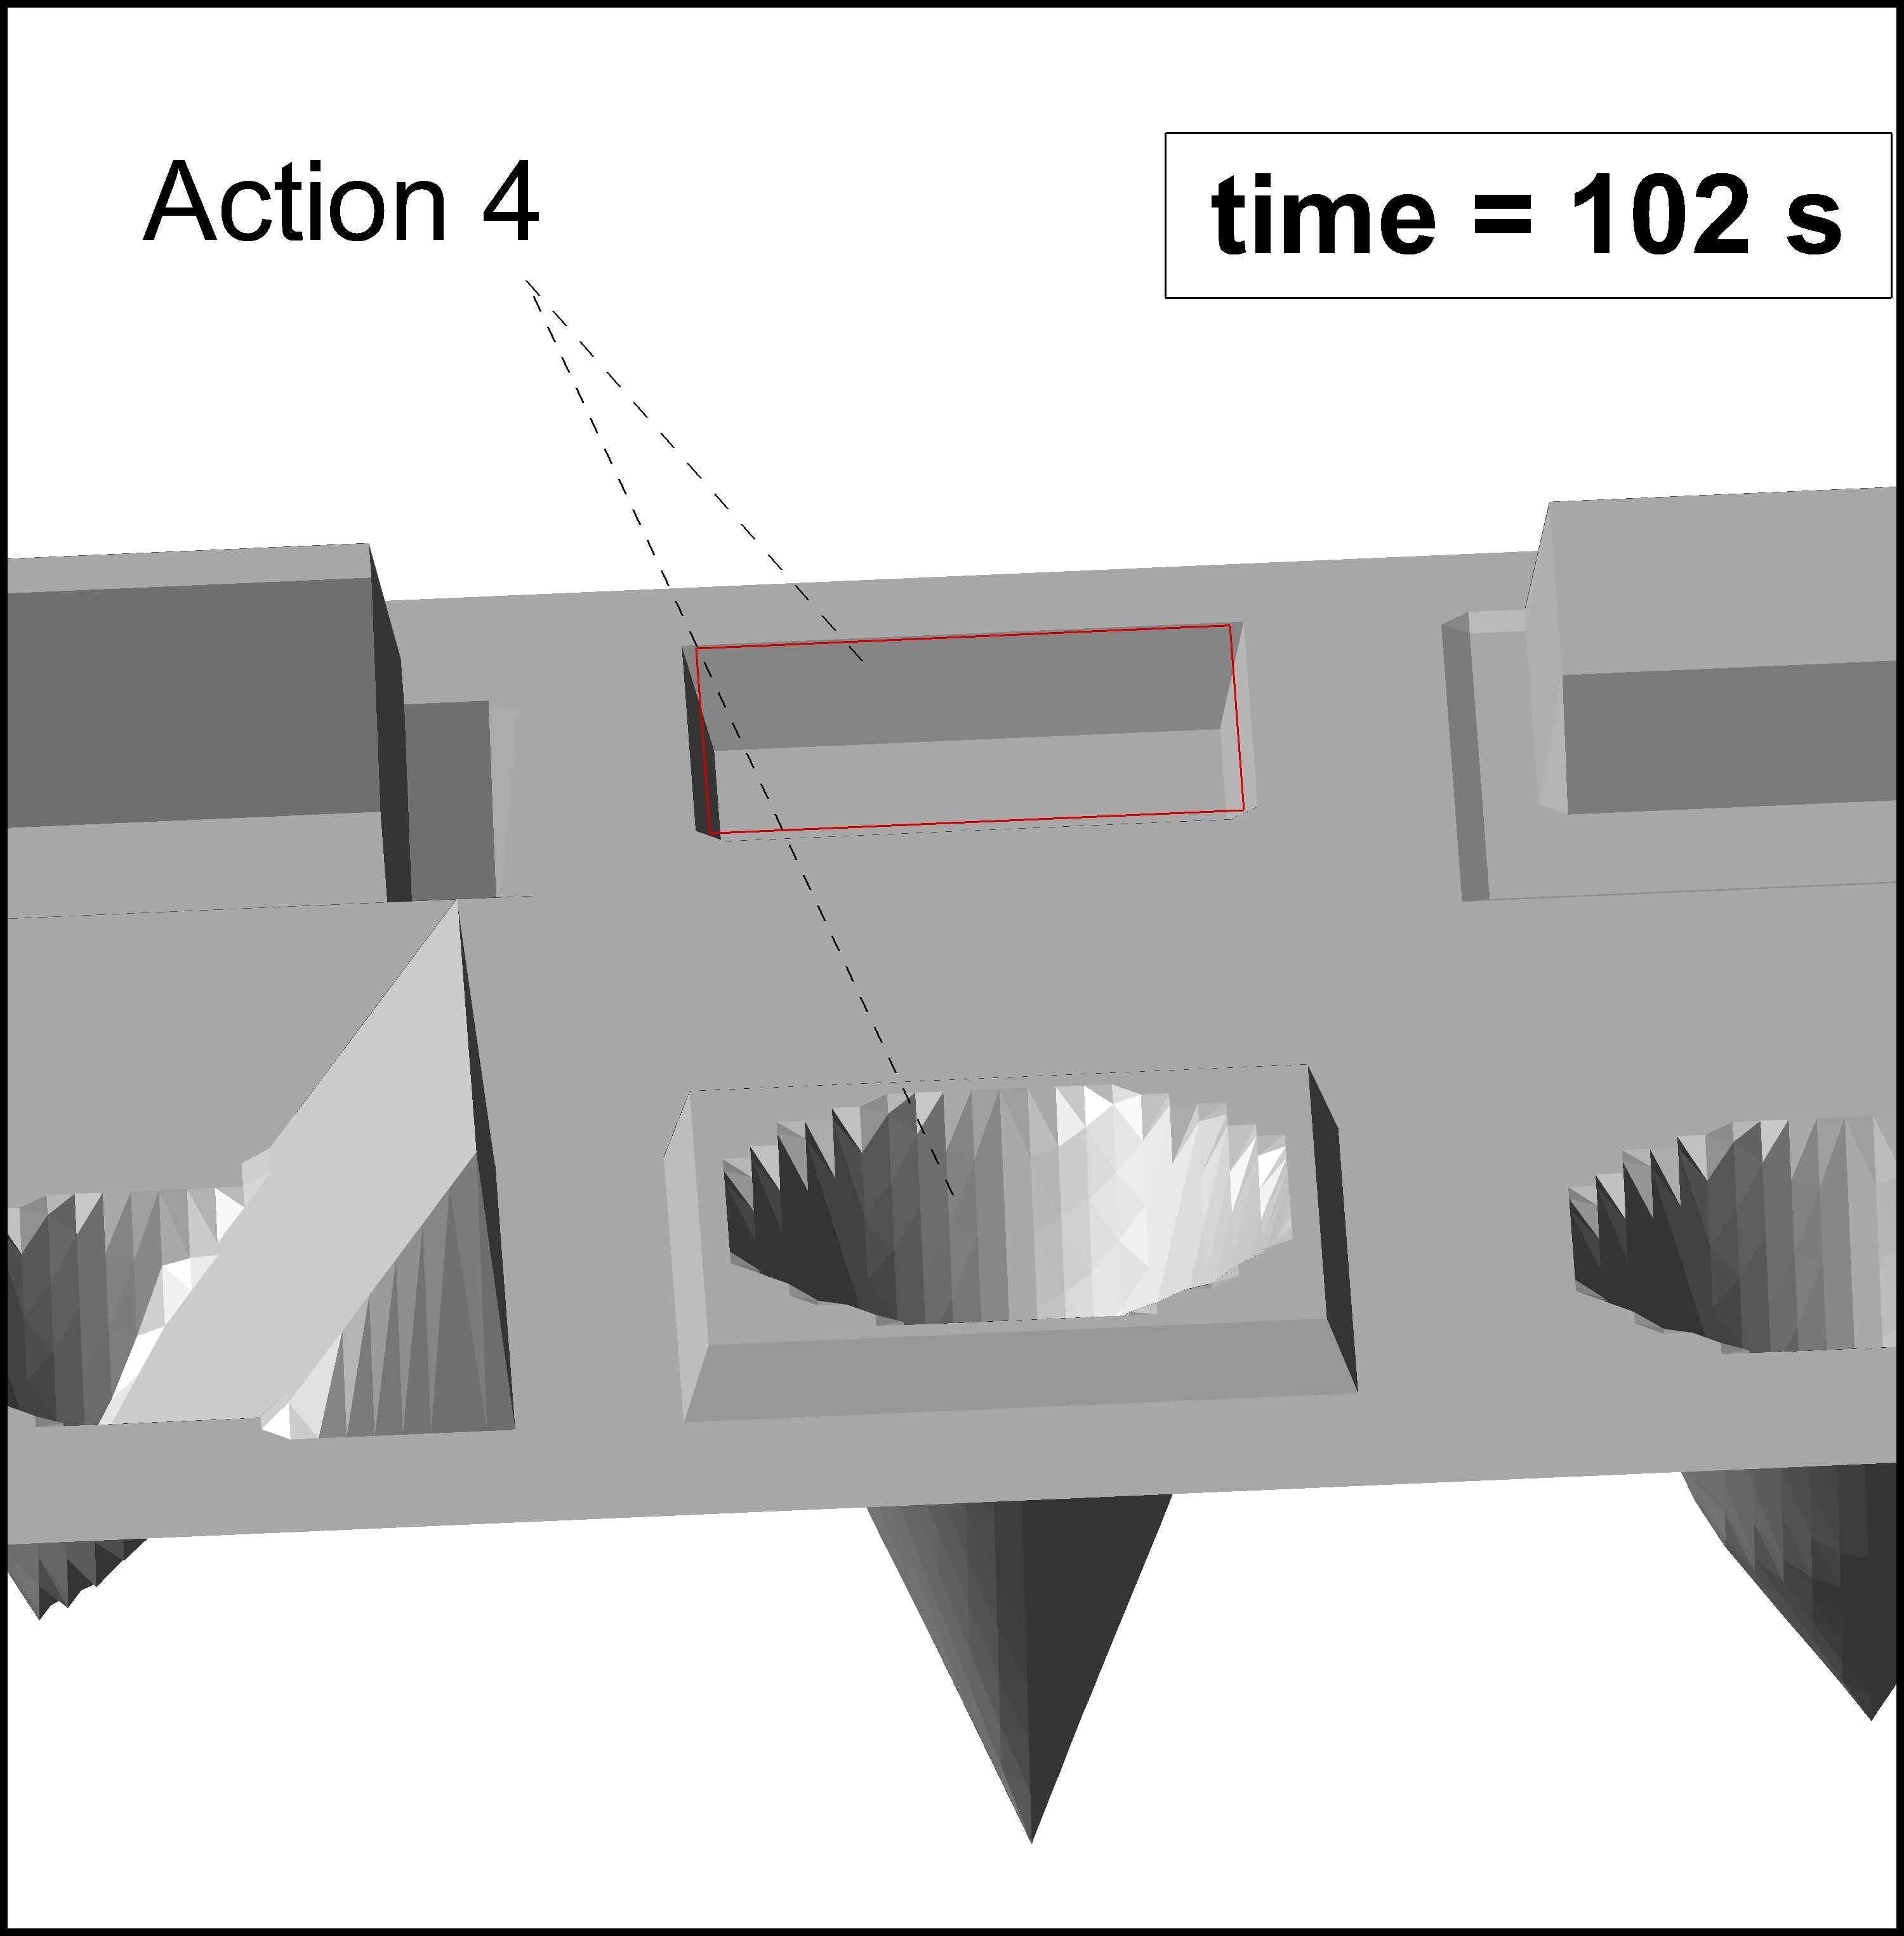
\includegraphics[width=0.45\textwidth]{img/Bild_Act4_102s.png}}\qquad
    \subfloat[dumping just
                          finished]{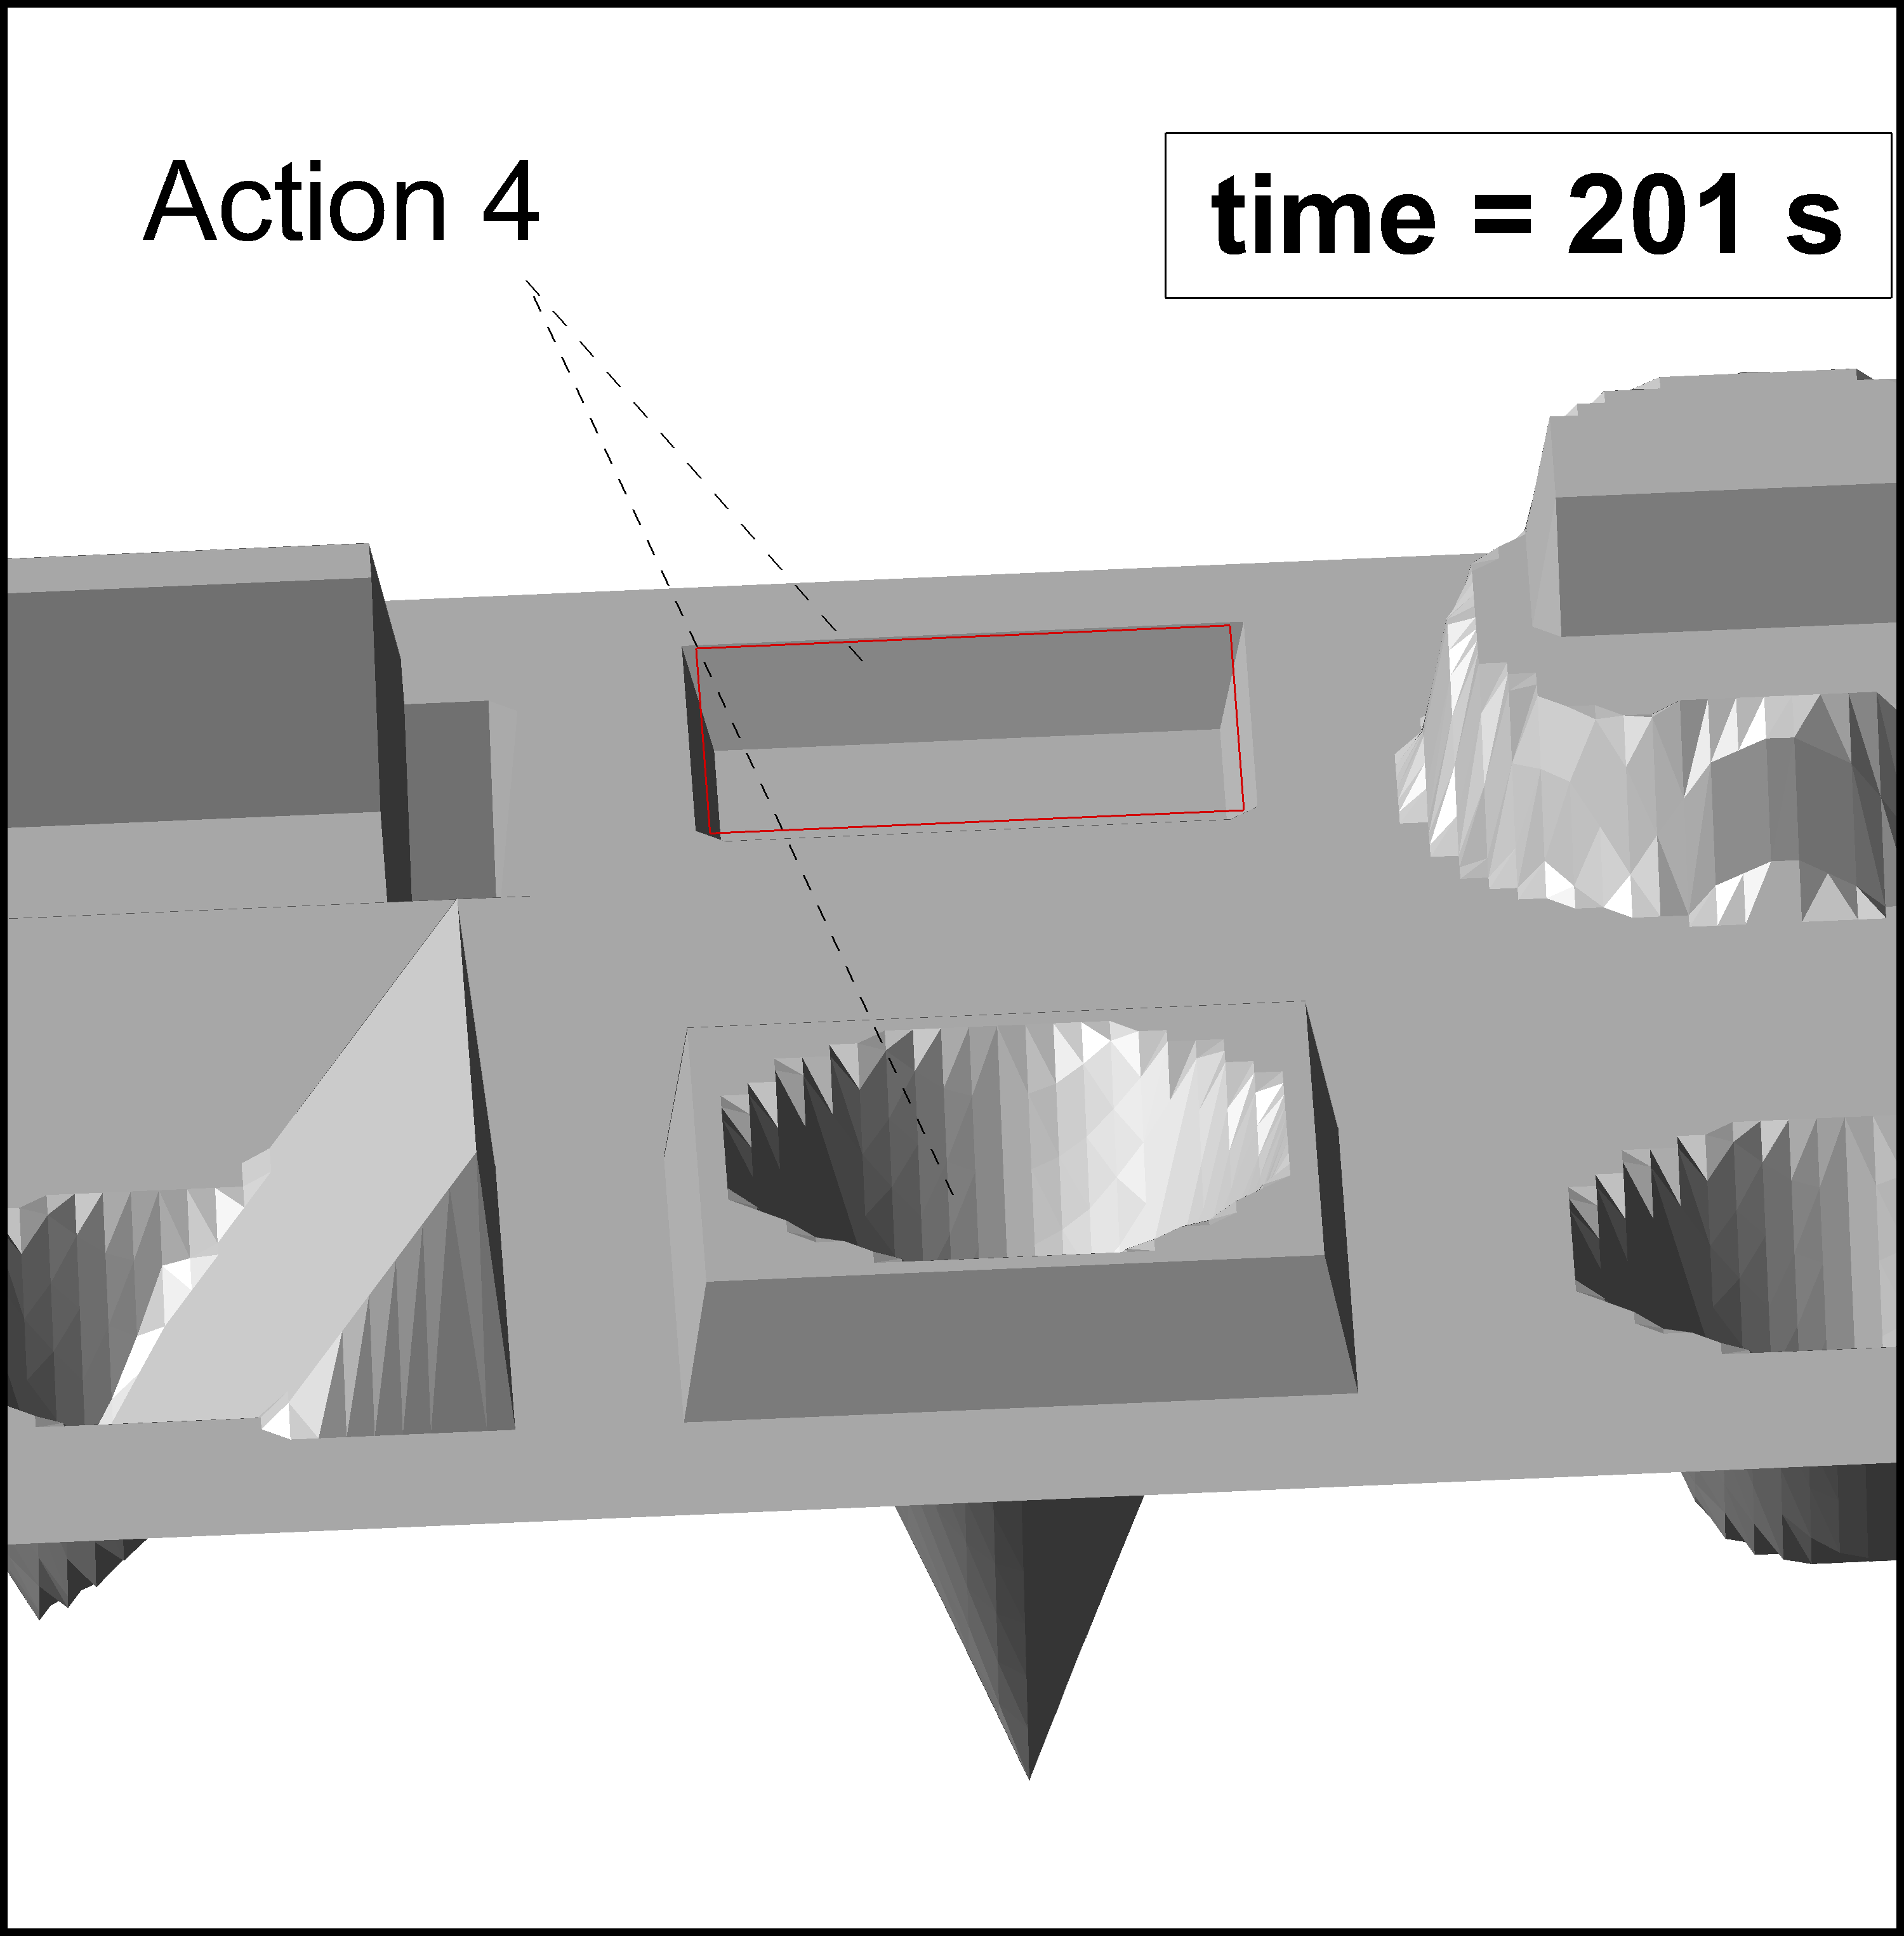
\includegraphics[width=0.45\textwidth]{img/Bild_Act4_201s.png}}
  \caption{Changes of the bottom while executing Action-4}
  \label{Act4}
\end{figure}

\newpage
Excerpt from the action file where the Action-4 is defined:
\\ \hspace*{3mm} \texttt{\small{/================================================================}}
\\ \hspace*{3mm} \texttt{\small{ACTION}}
\\ \hspace*{3mm} \texttt{\small{~~ActionType~~~~~~=~Dig\_by\_time}}
\\ \hspace*{3mm} \texttt{\small{~~TimeStart~~~~~~~=~~2000.01.01-00:00:02~~/~[yyyy.mm.dd-hh:mm:ss]}}
\\ \hspace*{3mm} \texttt{\small{~~TimeEnd~~~~~~~~~=~~2000.01.01-00:01:42~~/~[yyyy.mm.dd-hh:mm:ss]}}
\\ \hspace*{3mm}
\\ \hspace*{3mm} \texttt{\small{~~FieldDig~~~~~~~~=~~433\_ri\_middle\_high}}
\\ \hspace*{3mm} \texttt{\small{~~DigVolume~~~~~~~=~~529.0~~~~~~~~~~~~~~~~/~[m\textasciicircum3]}}
\\ \hspace*{3mm}
\\ \hspace*{3mm} \texttt{\small{~~FieldDump~~~~~~~=~~423\_le\_middle\_high}}
\\ \hspace*{3mm} \texttt{\small{~~DumpPlanar~~~~~~=~~FALSE}}
\\ \hspace*{3mm} \texttt{\small{~~DumpRate~~~~~~~~=~~0.005~~~~~~~~~~~~~~~~/~[m/s]}}
\\ \hspace*{3mm} \texttt{\small{ENDACTION}}
\\ \hspace*{3mm} \texttt{\small{/================================================================}}



% ******************************************************************
% ******************************************************************
% **                                                              **
% **                          Action-5                            **
% ******************************************************************
% ******************************************************************
\newpage
\subsection{Action-5: ActionType\, = \,Dig\_by\_time , ReferenceLevel = SECTIONS}
\label{ssec:E4Action5}
\textbf{Action-5 :}~~~\texttt{ActionType\,=\,Dig\_by\_time}~~~In the flield \texttt{434\_ri\_top},
beginning at simulation time 00:00:02, a volume of 529\,m$^3$ will be dredged during the next 100\,s.
Every node in the field will be lowered by 1.74\,m (fig.\,\ref{Act5}d).
Simultaneously the dredged material will be dumped into the field \texttt{424\_le\_top}.
The dumping will be executed completely while dredging because there is no setting for the dump rate.
\\Because of the setting \texttt{DumpPlanar=TRUE} and \texttt{ReferenceLevel=SECTIONS}, the
sections will be read from the file \texttt{\_DigRefLevel.dat} and used as reference level.
Therefore the bottom where the dumping happened is shaped like a sloped plane referring to the shape of
the reference level above the dump field (blue surface in fig.\,\ref{refl3D}).
\\
\begin{figure}[H]
  \centering
    \subfloat[]                    {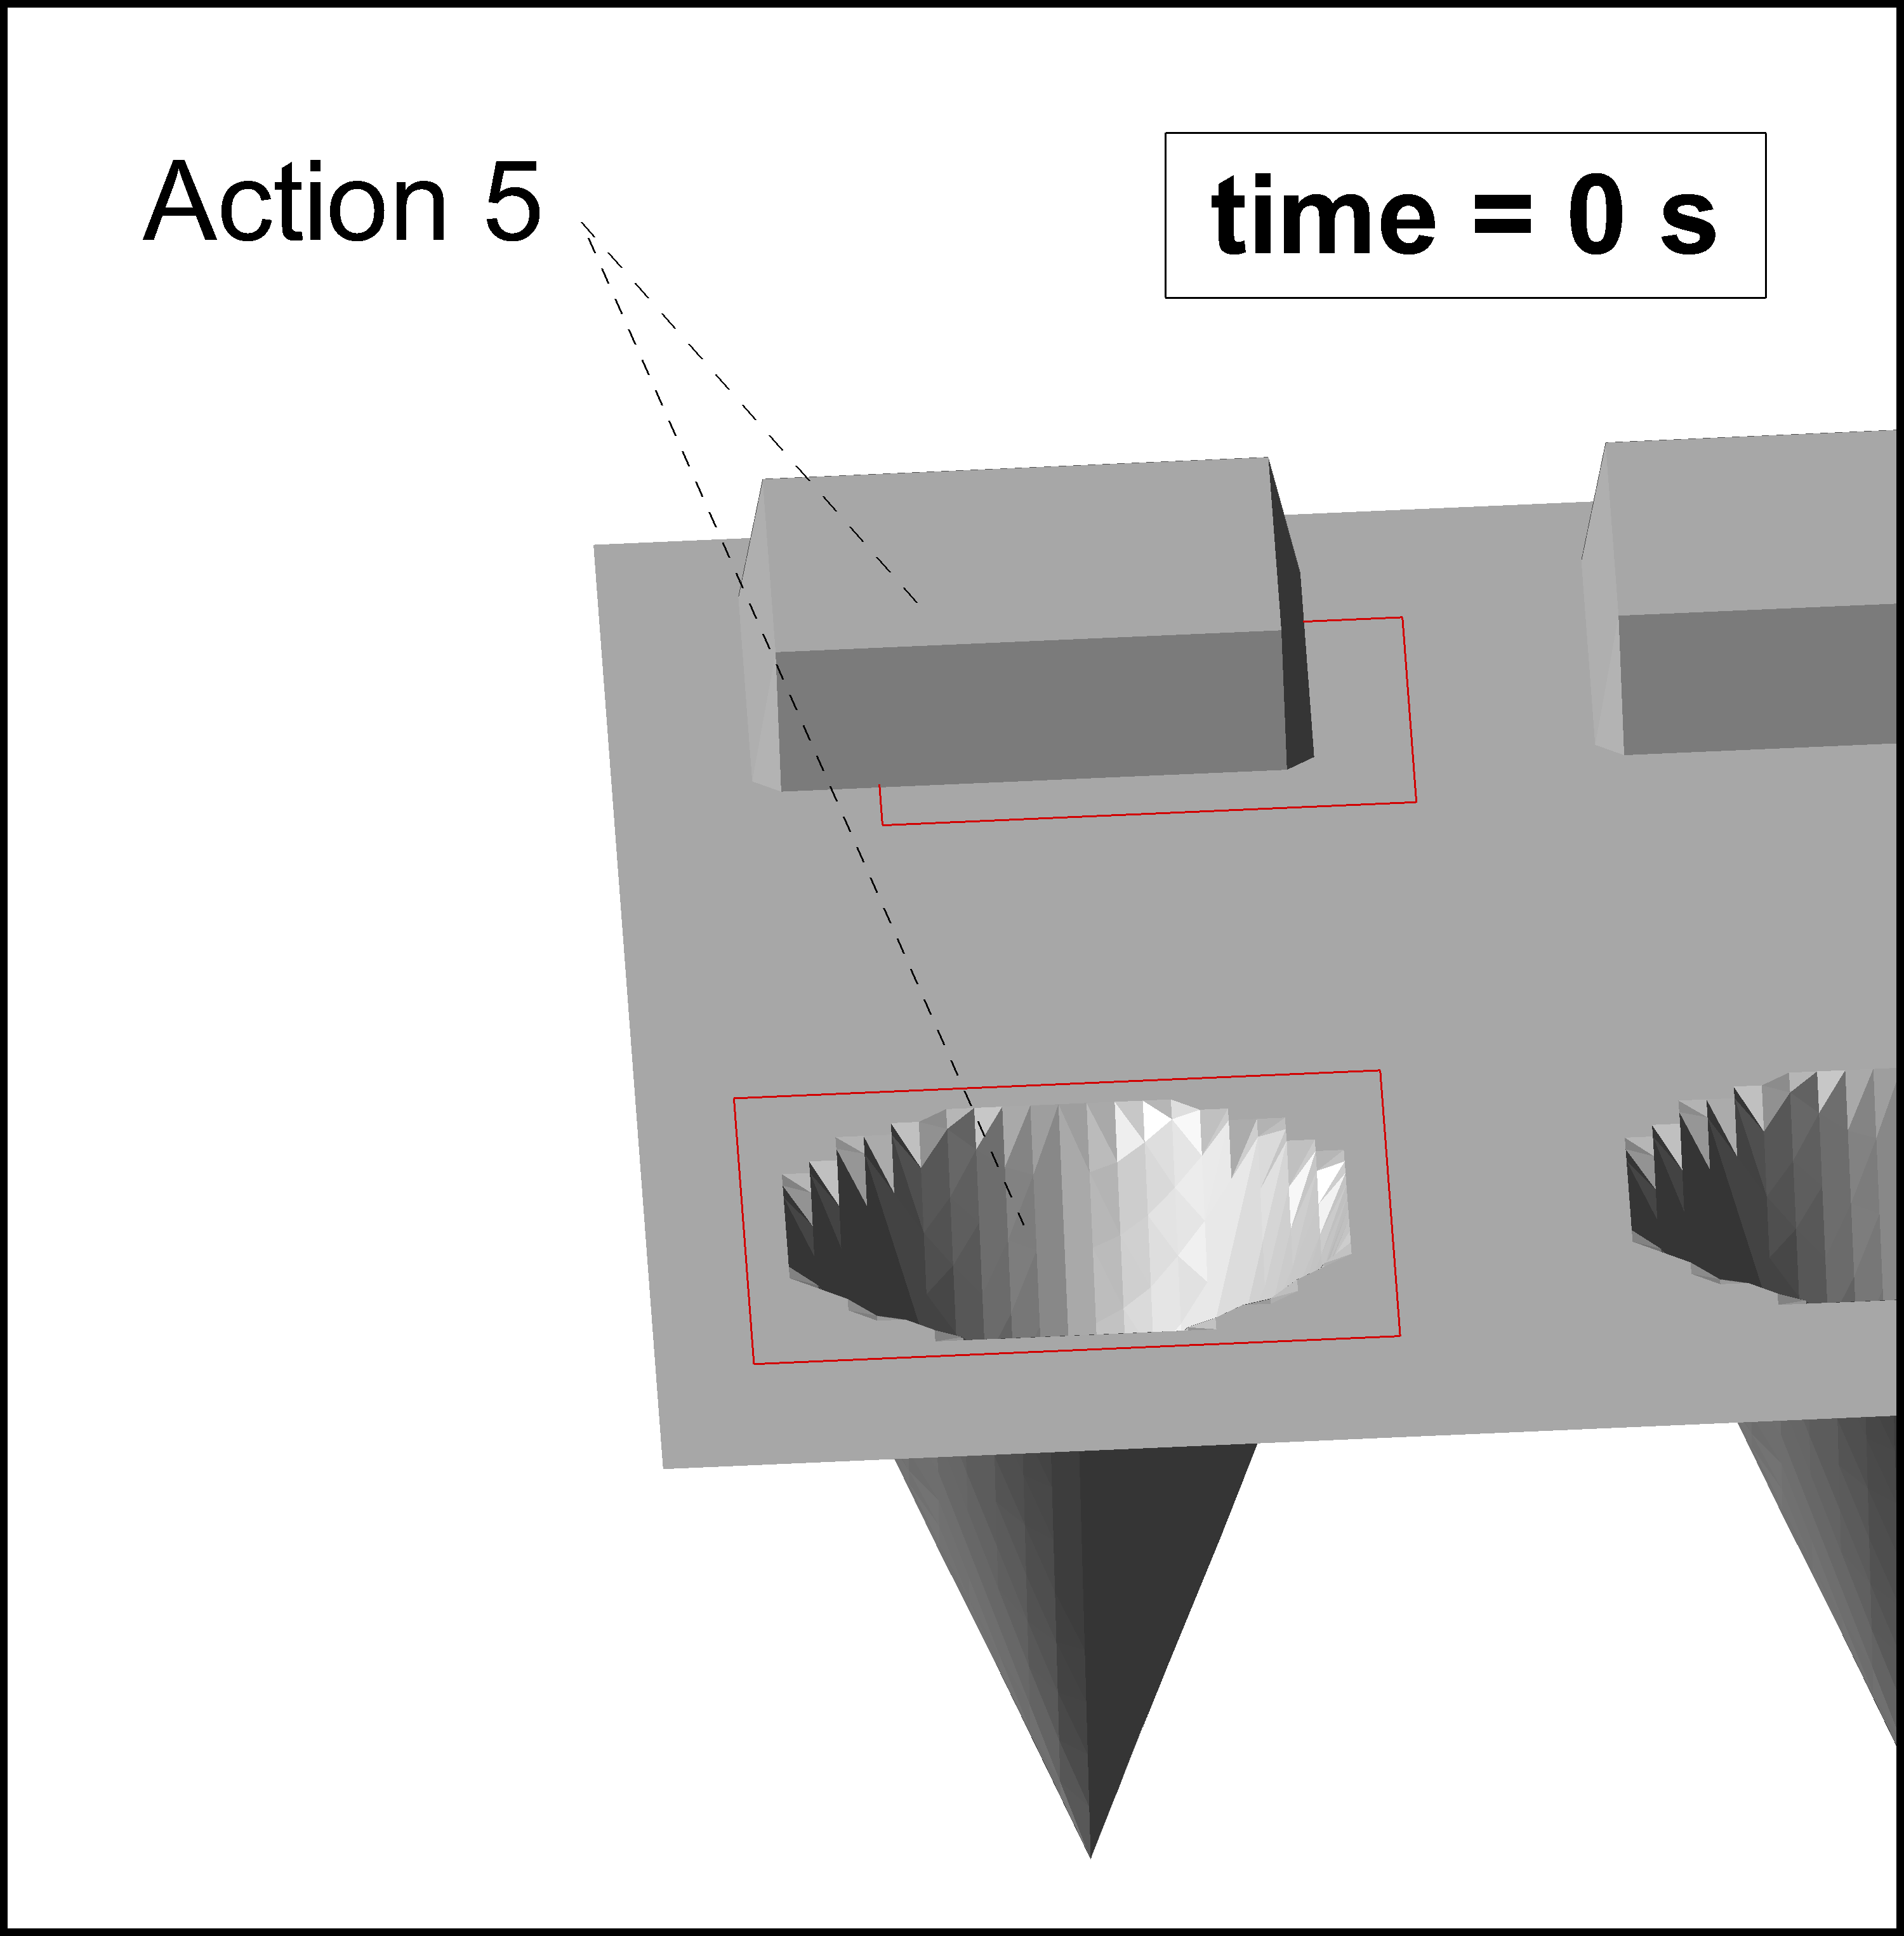
\includegraphics[width=0.45\textwidth]{img/Bild_Act5_000s.png}}\qquad
    \subfloat[dredging and dumping]{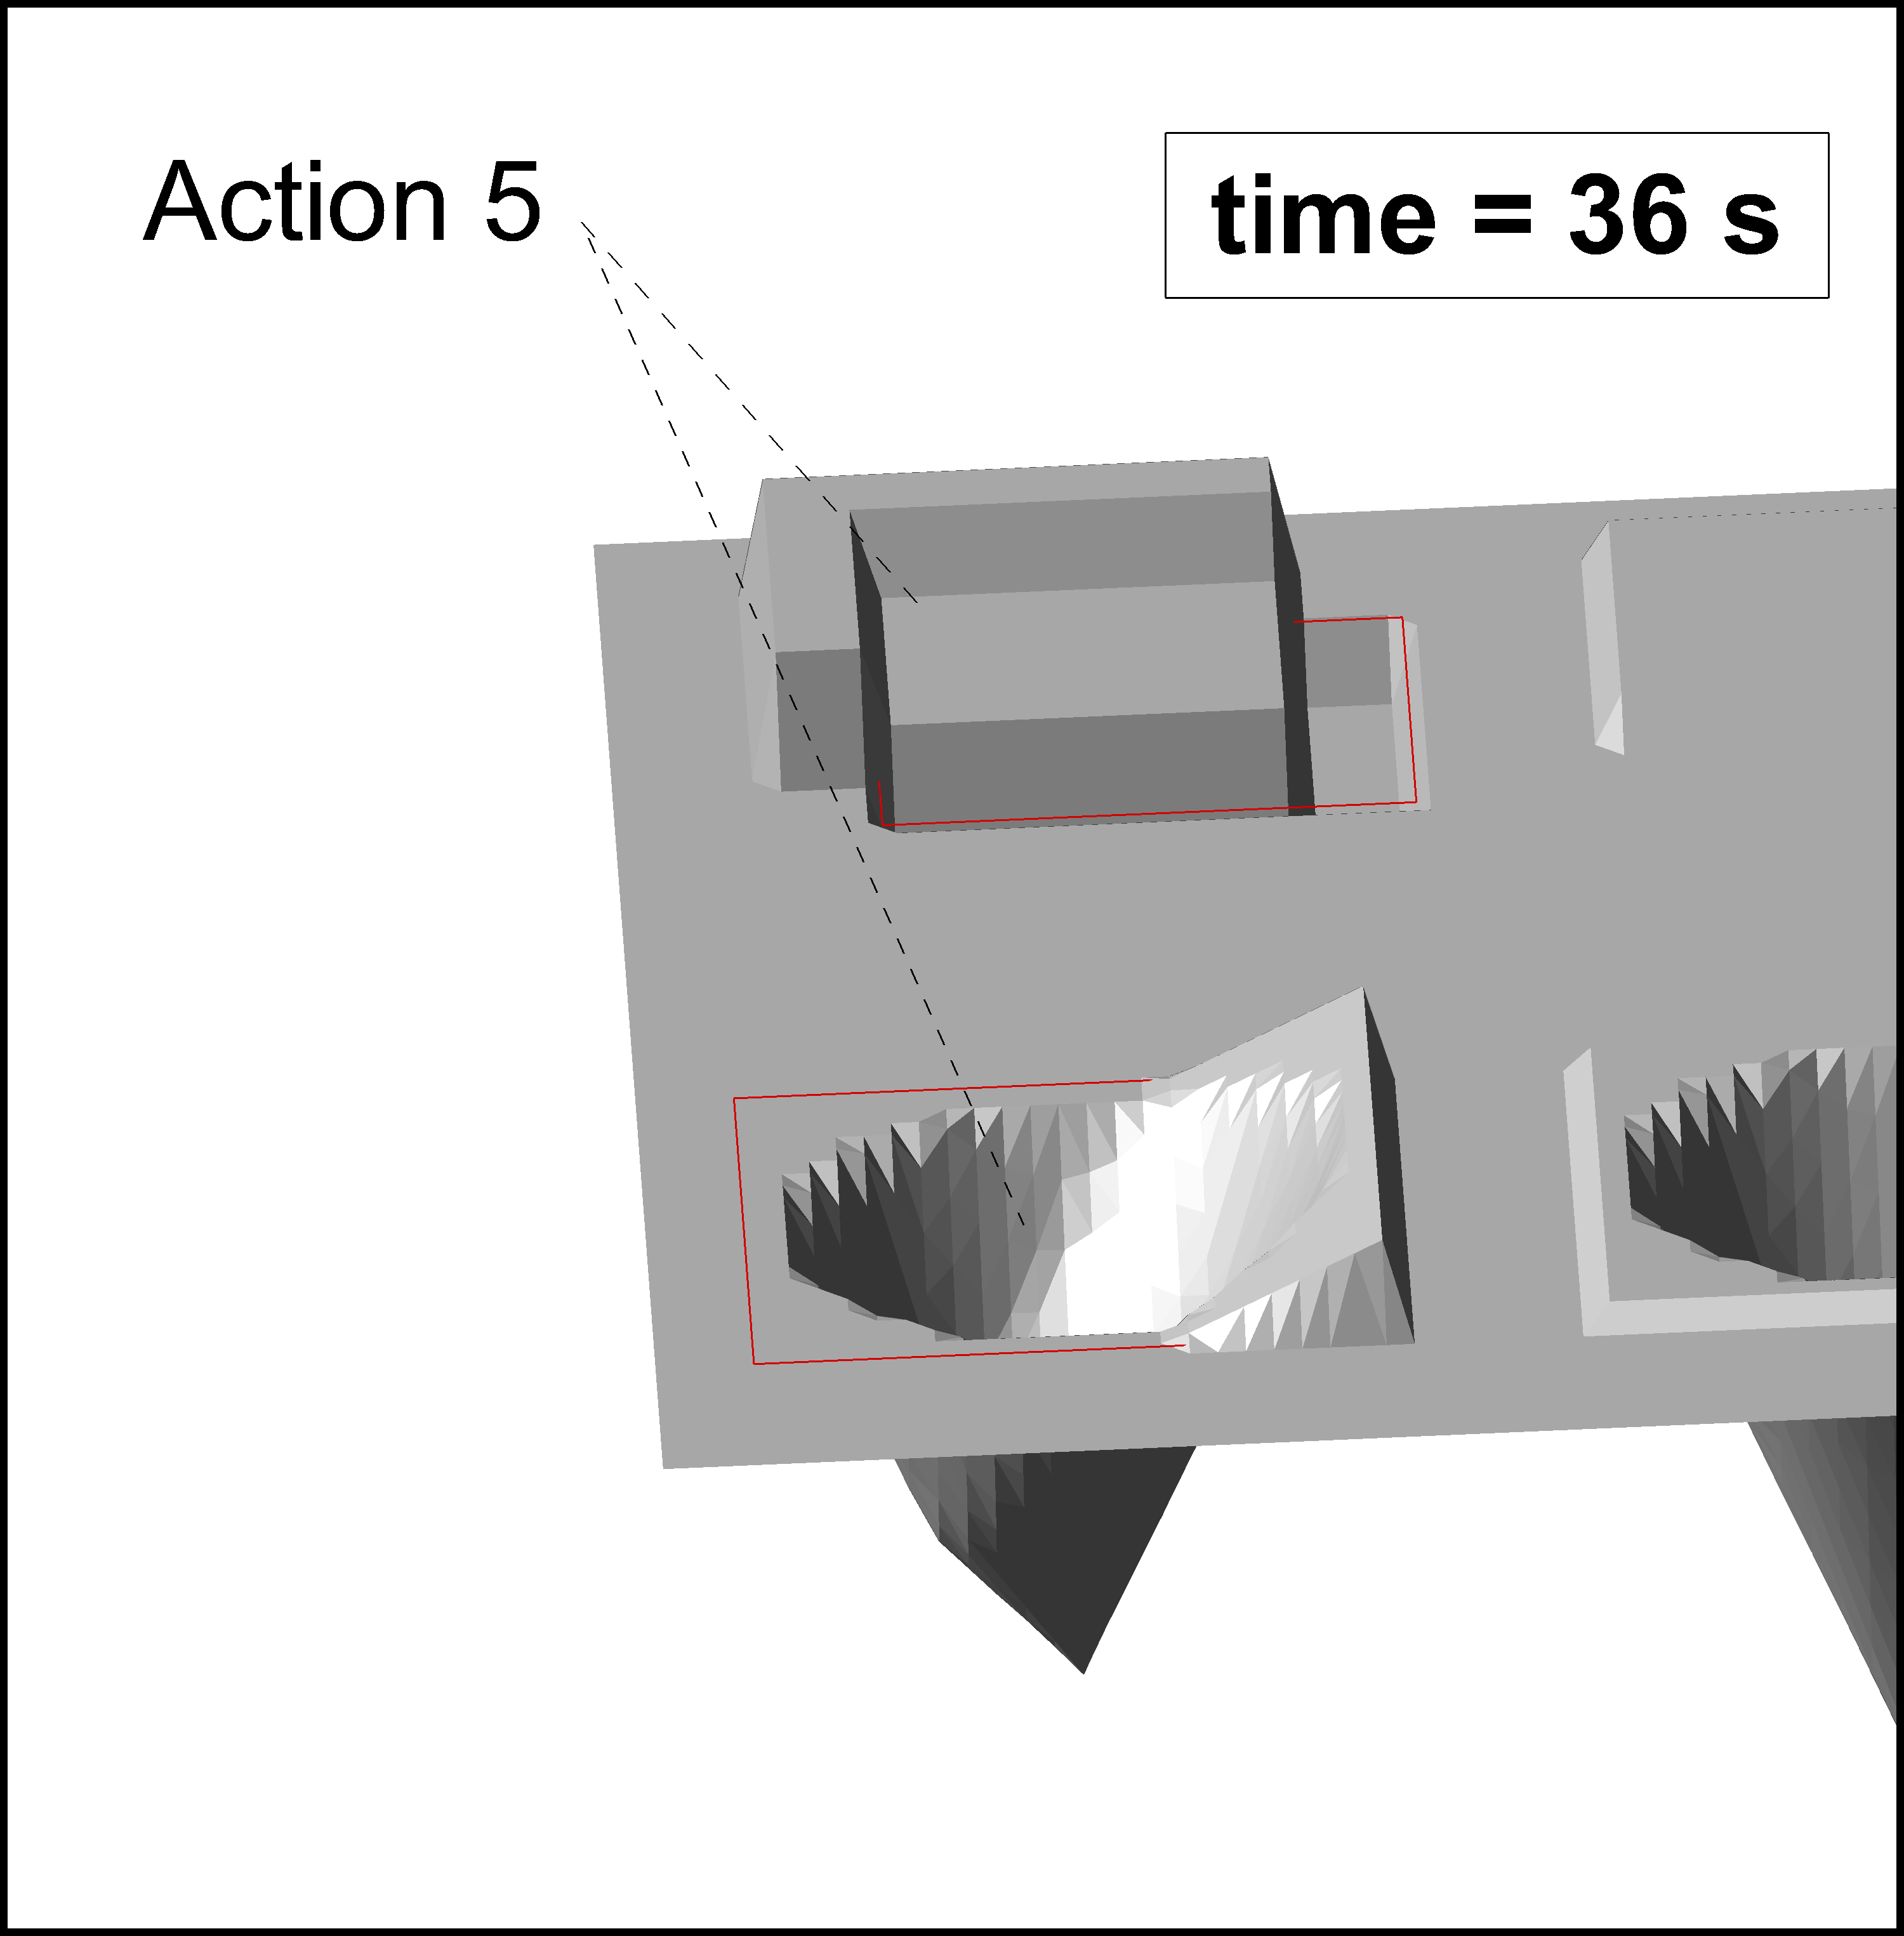
\includegraphics[width=0.45\textwidth]{img/Bild_Act5_036s.png}}\qquad
    \subfloat[dredging and dumping]{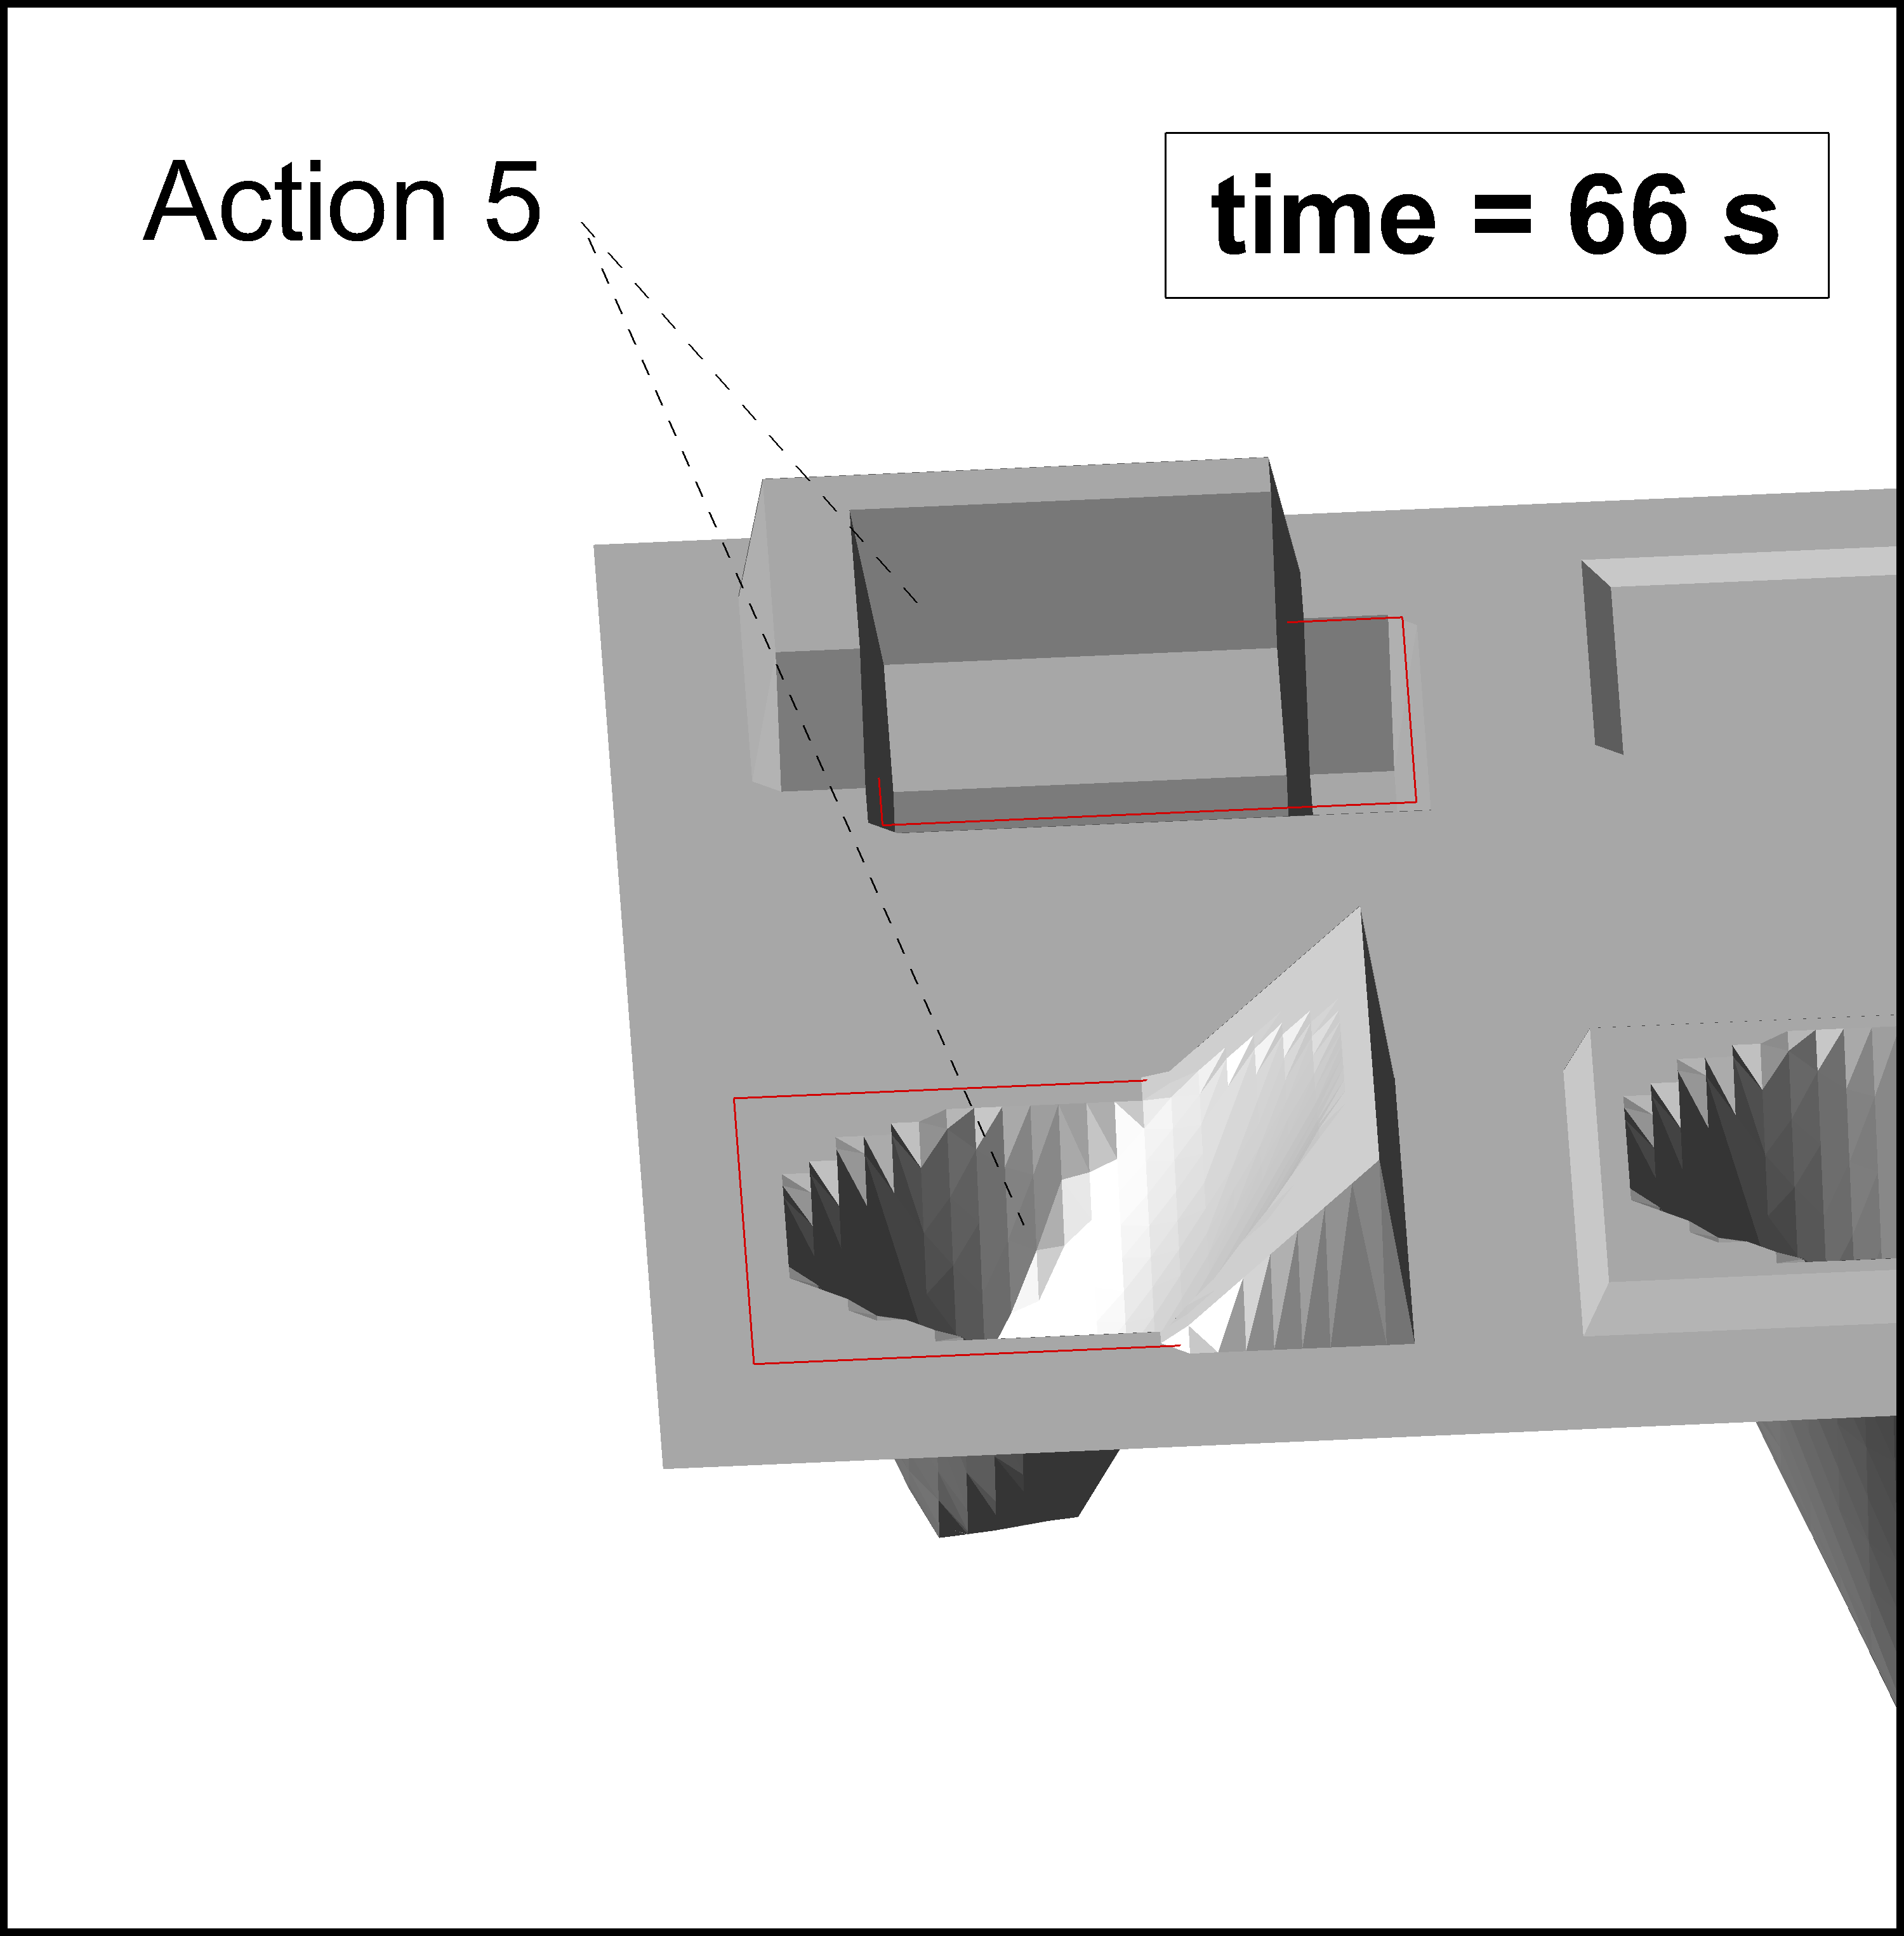
\includegraphics[width=0.45\textwidth]{img/Bild_Act5_066s.png}}\qquad
    \subfloat[dredging and dumping
                     just finished]{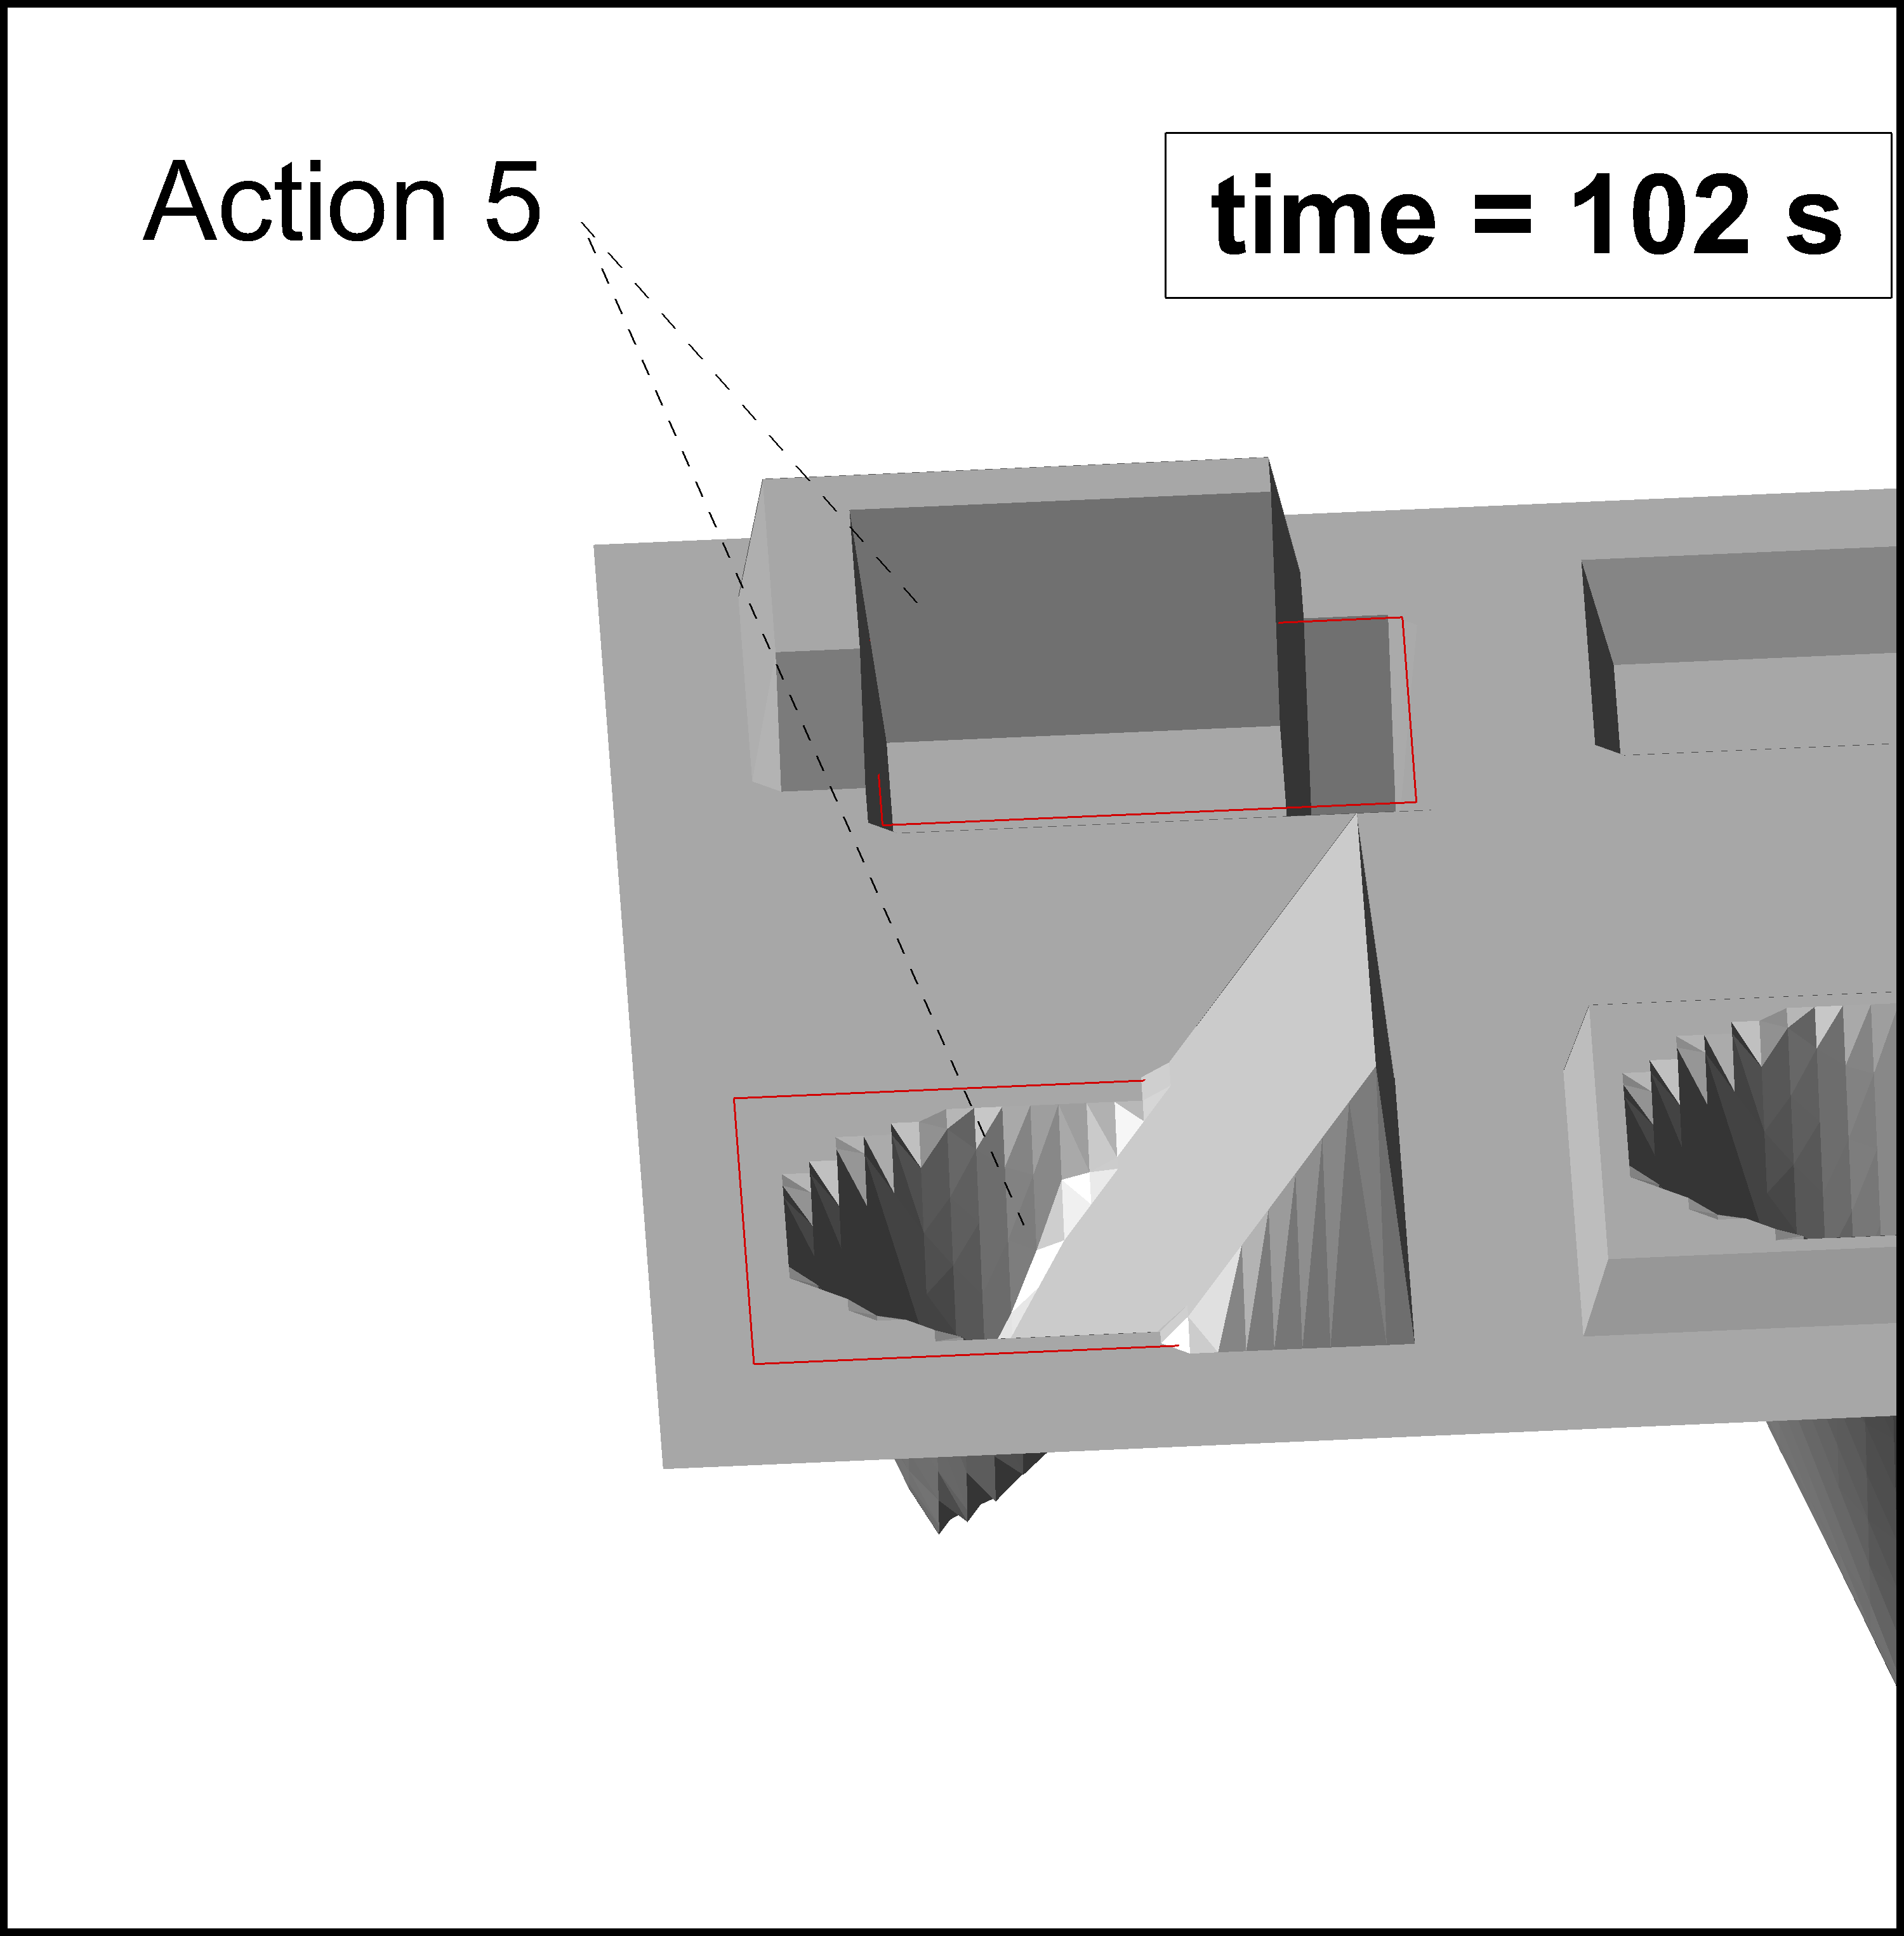
\includegraphics[width=0.45\textwidth]{img/Bild_Act5_102s.png}}
  \caption{Changes of the bottom while executing Action-5}
  \label{Act5}
\end{figure}

\newpage
Excerpt from the action file where the Action-5 is defined:
\\ \hspace*{3mm} \texttt{\small{/================================================================}}
\\ \hspace*{3mm} \texttt{\small{ACTION}}
\\ \hspace*{3mm} \texttt{\small{~~ActionType~~~~~~=~Dig\_by\_time}}
\\ \hspace*{3mm} \texttt{\small{~~ReferenceLevel~~=~~SECTIONS}}
\\ \hspace*{3mm} \texttt{\small{~~TimeStart~~~~~~~=~~2000.01.01-00:00:02~~/~[yyyy.mm.dd-hh:mm:ss]}}
\\ \hspace*{3mm} \texttt{\small{~~TimeEnd ~~~~~~~~=~~2000.01.01-00:01:42~~/~[yyyy.mm.dd-hh:mm:ss]}}
\\ \hspace*{3mm}
\\ \hspace*{3mm} \texttt{\small{~~FieldDig~~~~~~~~=~~434\_ri\_top}}
\\ \hspace*{3mm} \texttt{\small{~~DigVolume~~~~~~~=~~529.0~~~~~~~~~~~~~~~~/~[m\textasciicircum3]}}
\\ \hspace*{3mm}
\\ \hspace*{3mm} \texttt{\small{~~FieldDump~~~~~~~=~~424\_le\_top}}
\\ \hspace*{3mm} \texttt{\small{~~DumpPlanar~~~~~~=~~TRUE}}
\\ \hspace*{3mm} \texttt{\small{ENDACTION}}
\\ \hspace*{3mm} \texttt{\small{/================================================================}}


% ******************************************************************
% ******************************************************************
% **                                                              **
% **                          Action-6                            **
% ******************************************************************
% ******************************************************************
\newpage
\subsection{Action-6: ActionType\, = \,Backfill\_to\_level , ReferenceLevel = GRID}
\label{ssec:E4Action6}
\textbf{Action-6 :}~~~\texttt{ActionType\,=\,Backfill\_to\_level}~~~begins at simulation time 00:02:52.
During the next 90\,s the nodes in the flield \texttt{532\_ri\_middle\_low\_2} are elevated to the
height: reference level minus \texttt{CritDepth}.\\
Because of the setting \texttt{~ReferenceLevel\,=\,GRID~} the surface which is available
in the \textsc{Geometry File} is used as reference level.
Although Nestor is now coupled to telemac2d it operates internally in the single grain mode. Because of this
\texttt{~GrainClass\,=\,1.0~} must be set.\\
\\
There is the option to control the backfilling by rate, to do so use the keyword \texttt{~DumpRate~}.\\
\\
As a result, the bottom where the back filling happened, is shaped like a spherical segment referring to the shape of
the reference level (grey surface in fig.\,\ref{refl3D}).\\
\\
\begin{figure}[H]
  \centering
    \subfloat[]                   {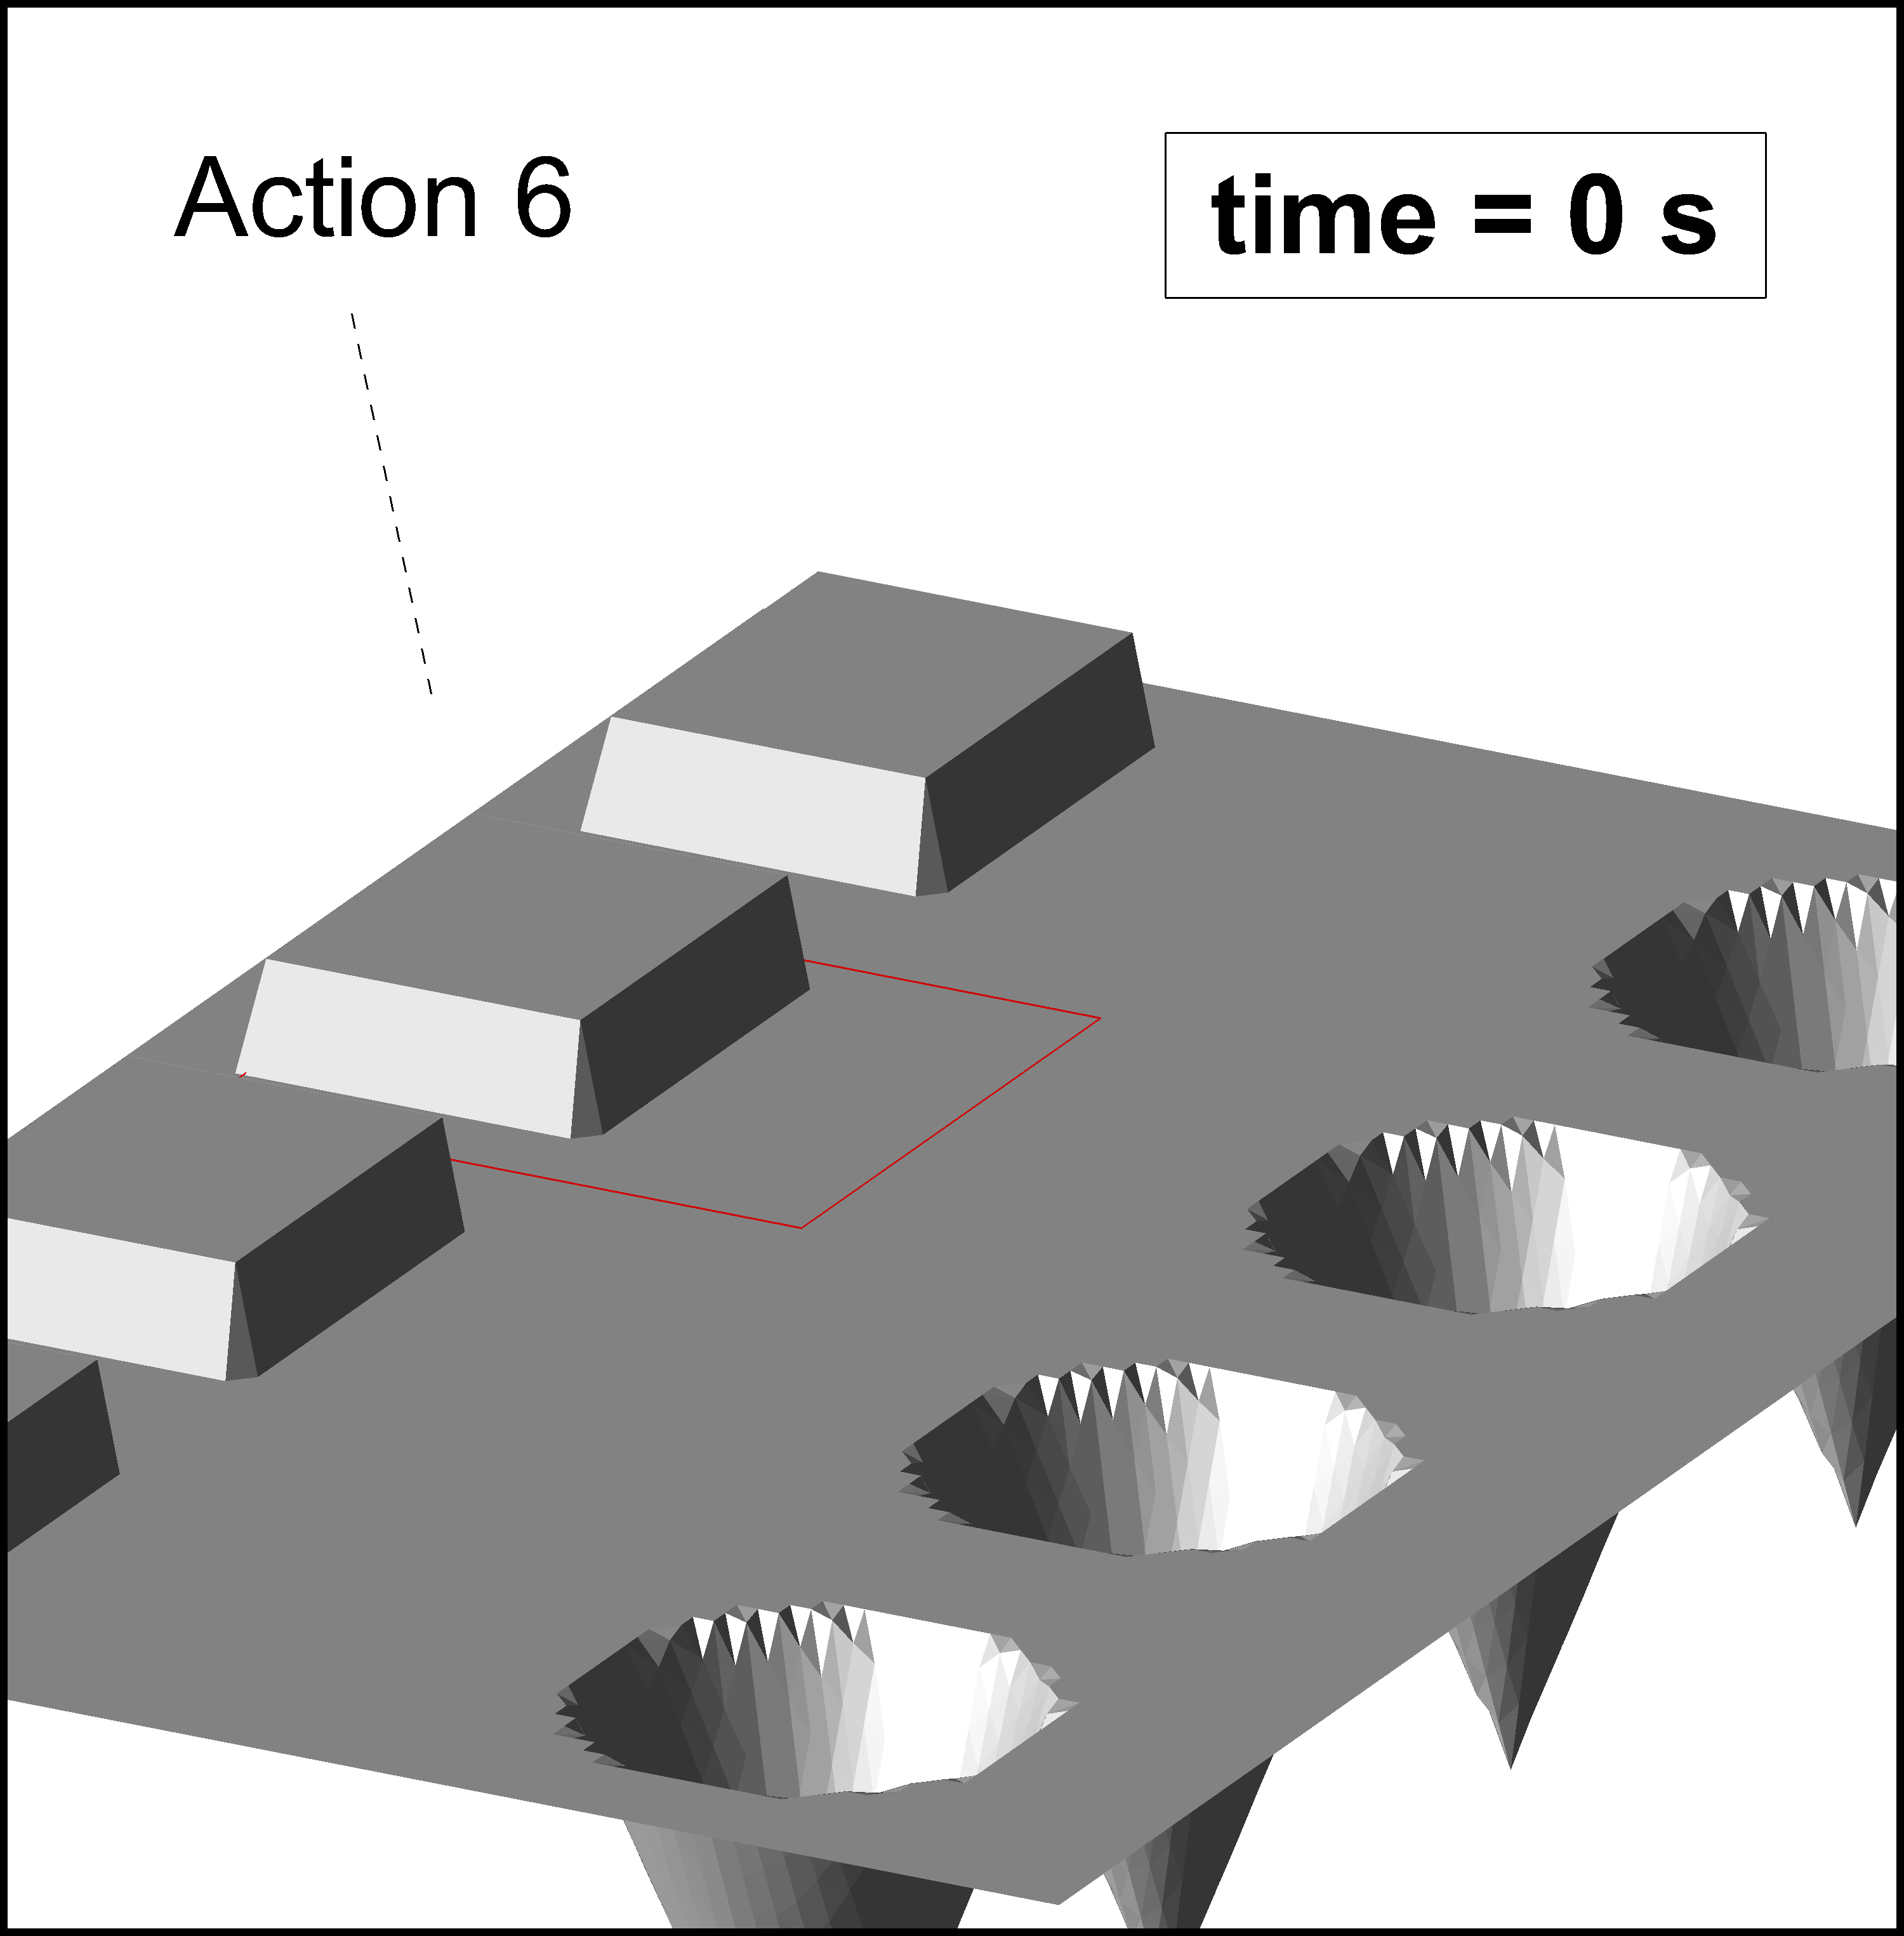
\includegraphics[width=0.45\textwidth]{img/Bild_Act6_000s.png}}\qquad
    \subfloat[just before dumping]{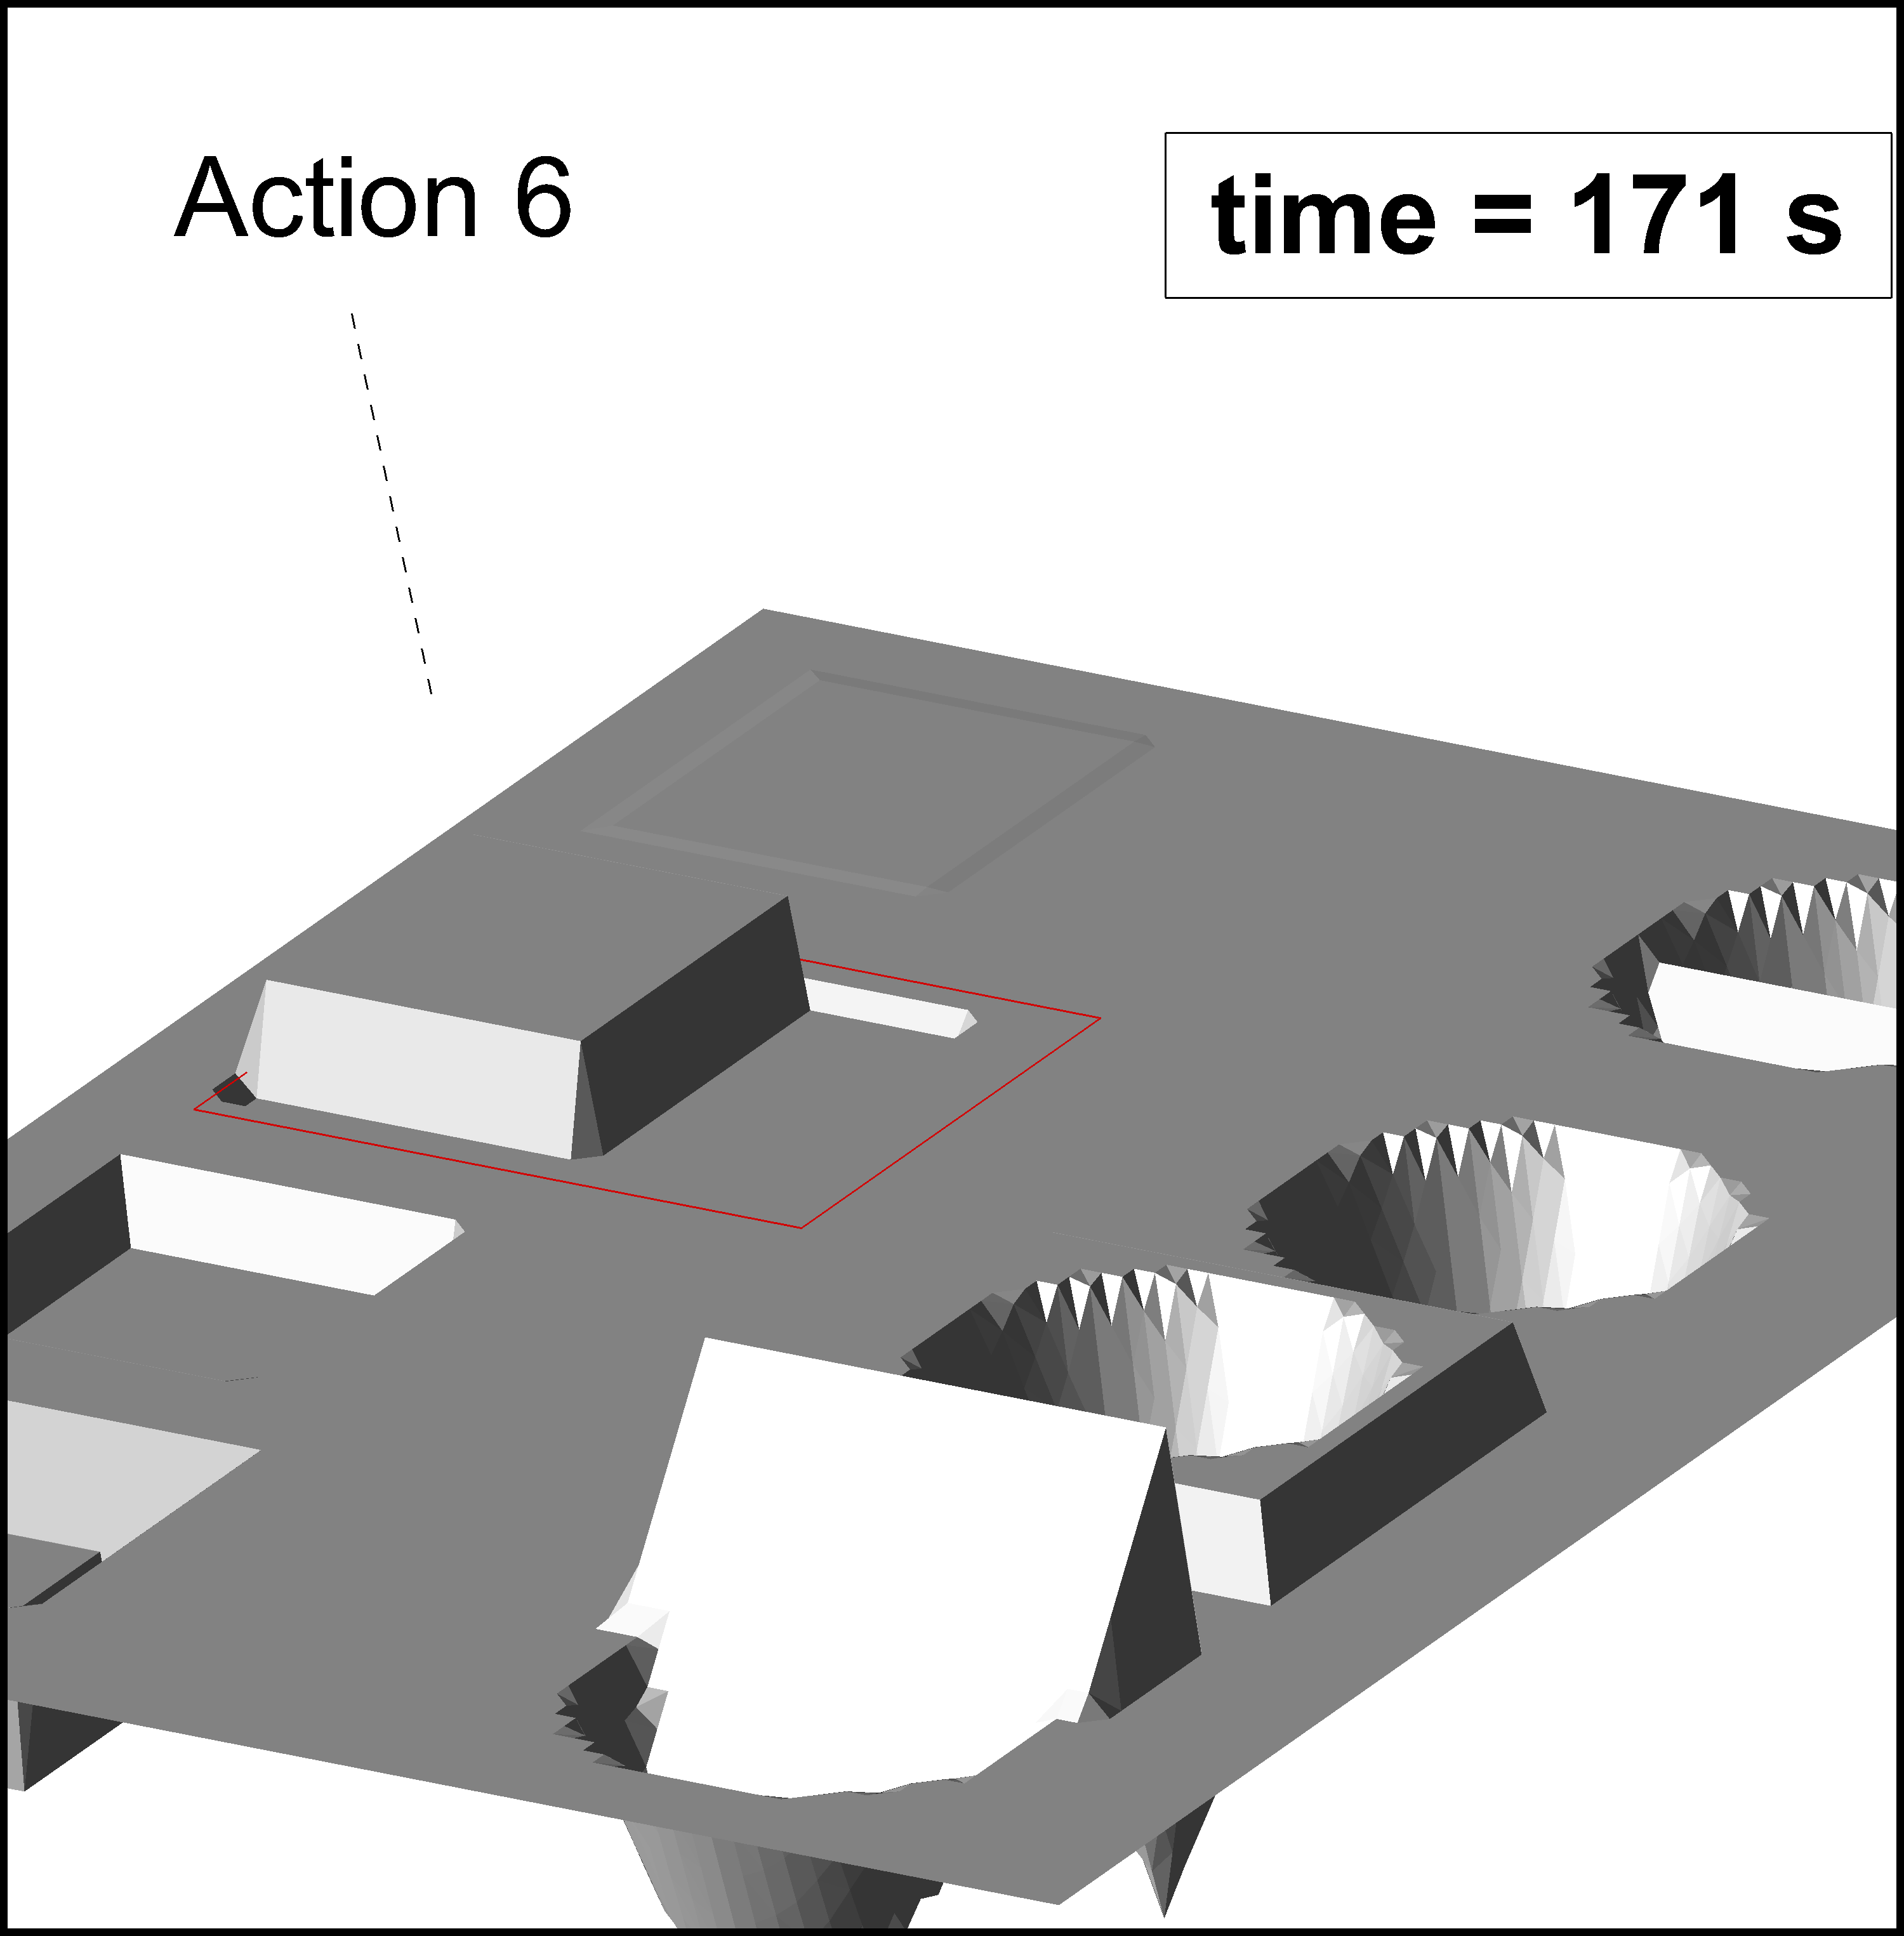
\includegraphics[width=0.45\textwidth]{img/Bild_Act6_171s.png}}\qquad
    \subfloat[dumping]            {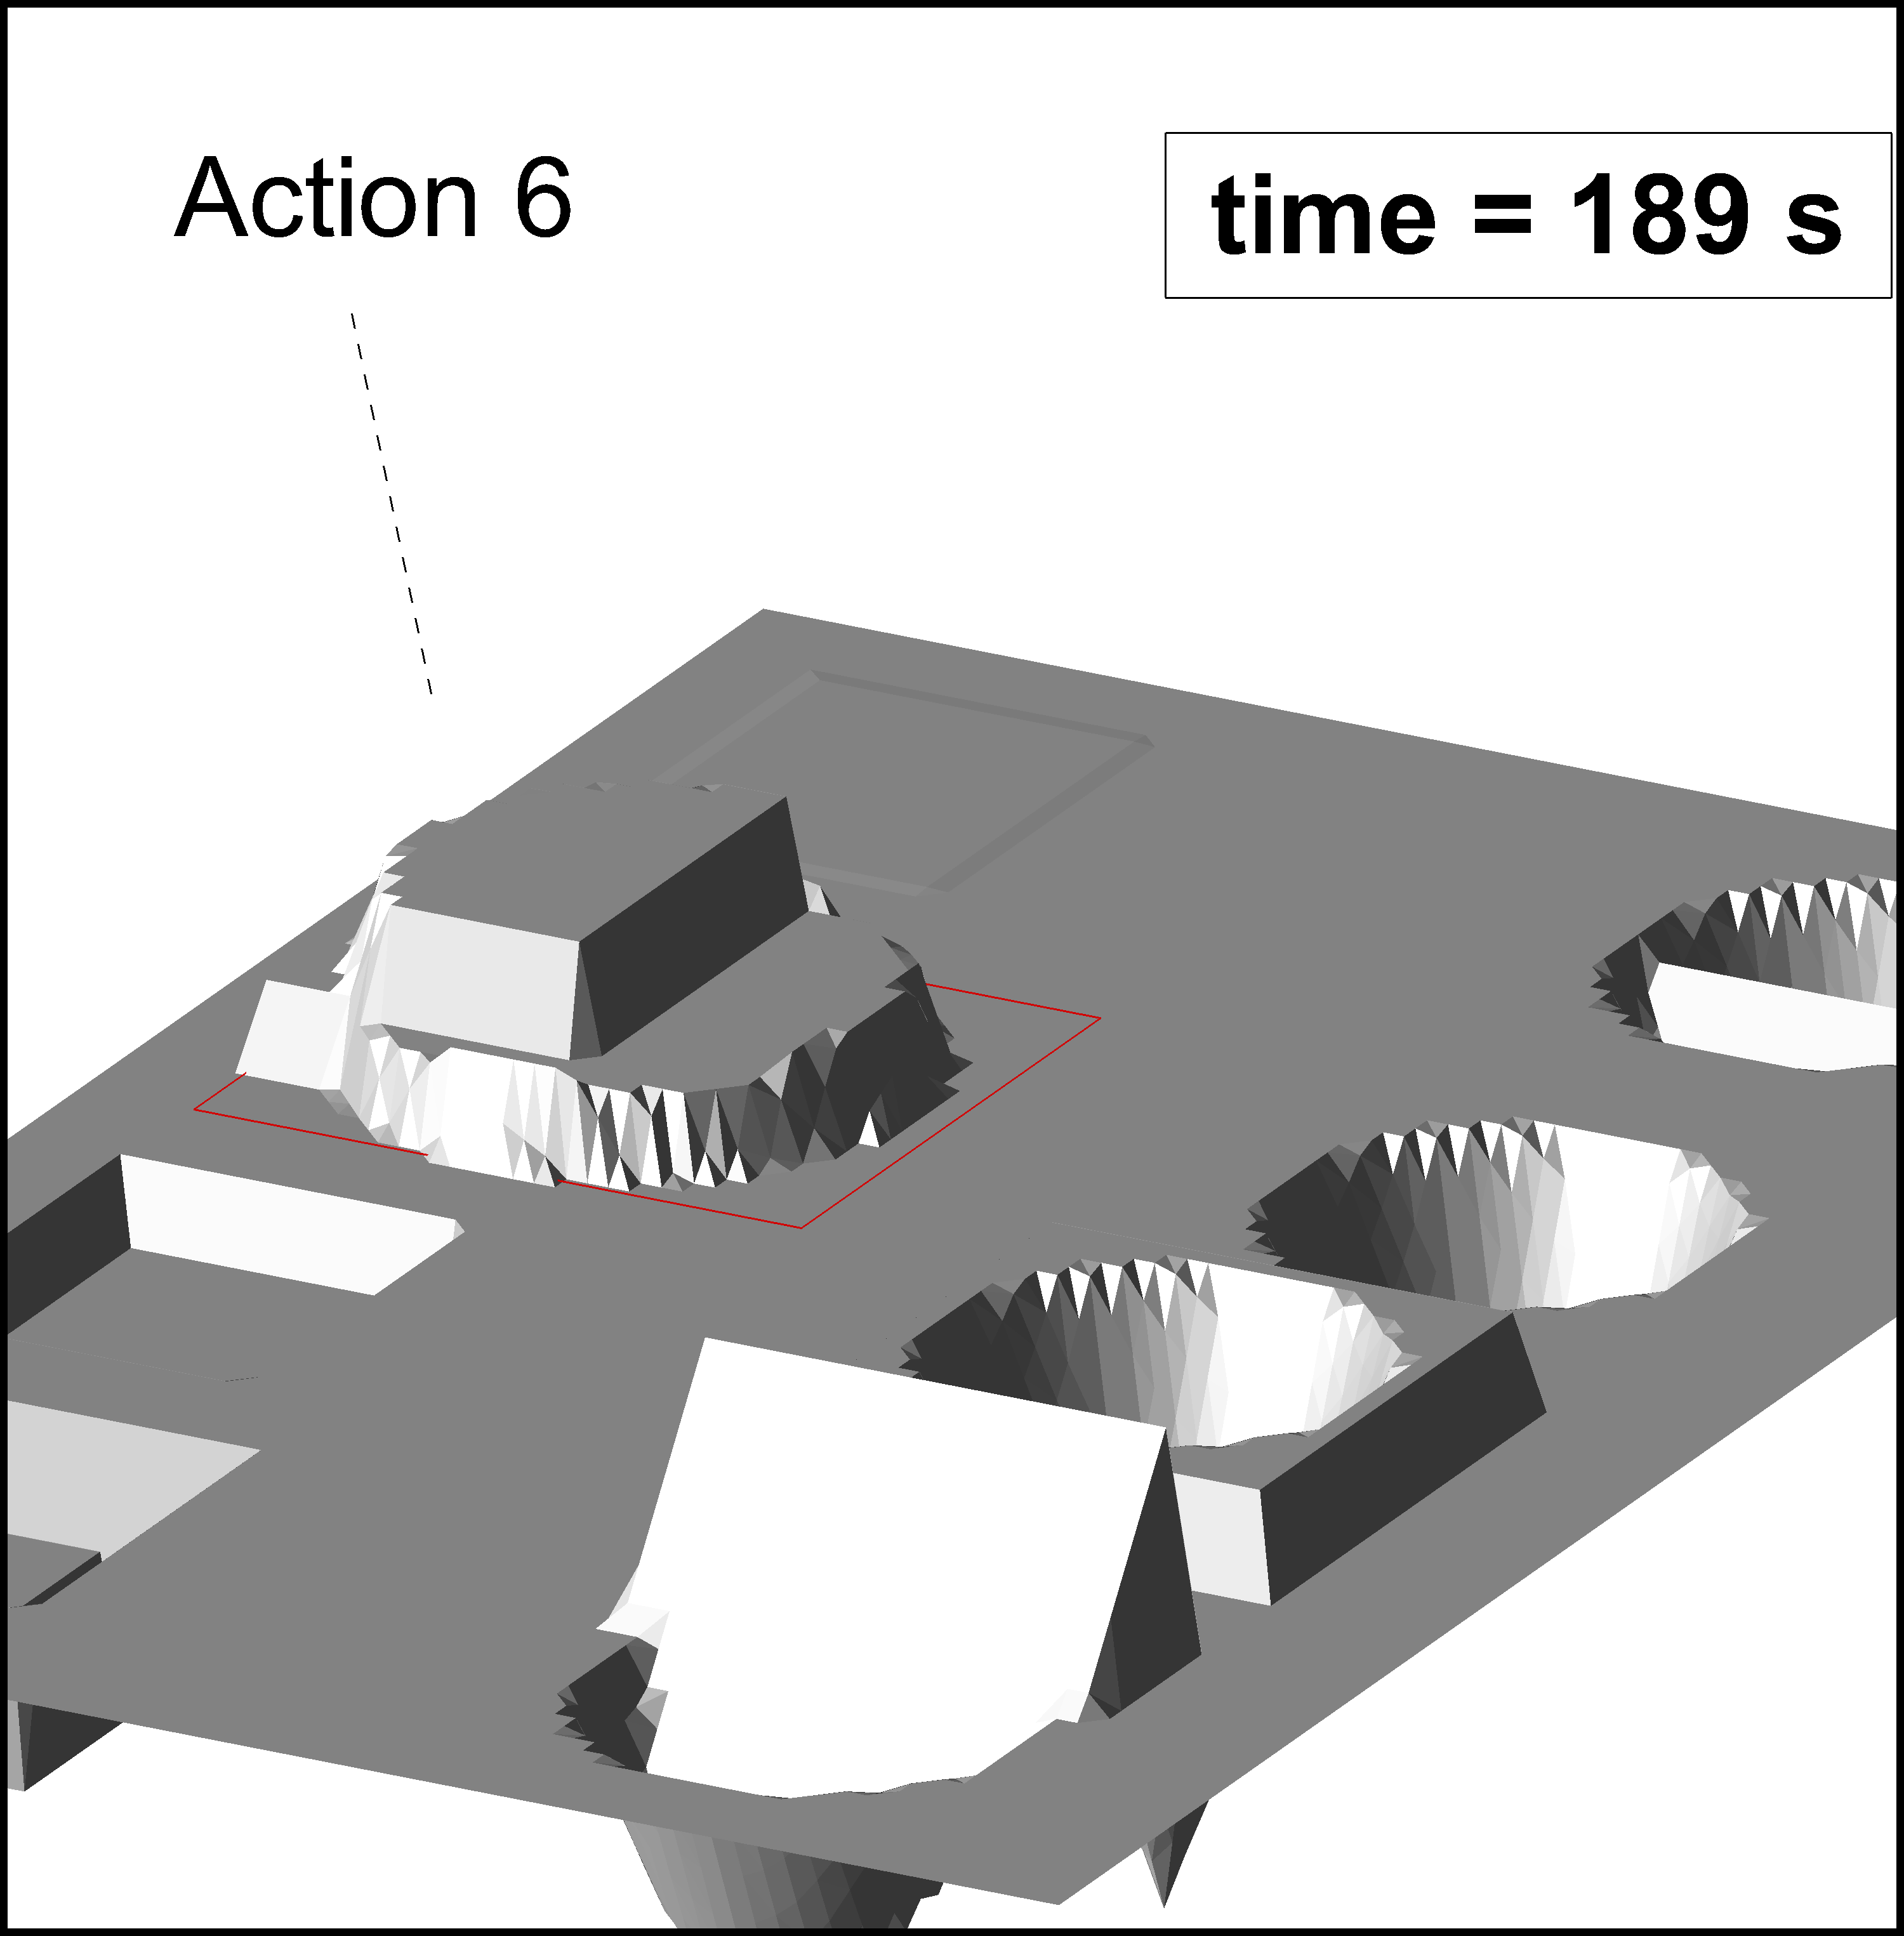
\includegraphics[width=0.45\textwidth]{img/Bild_Act6_189s.png}}\qquad
    \subfloat[just finished dumping
                                 ]{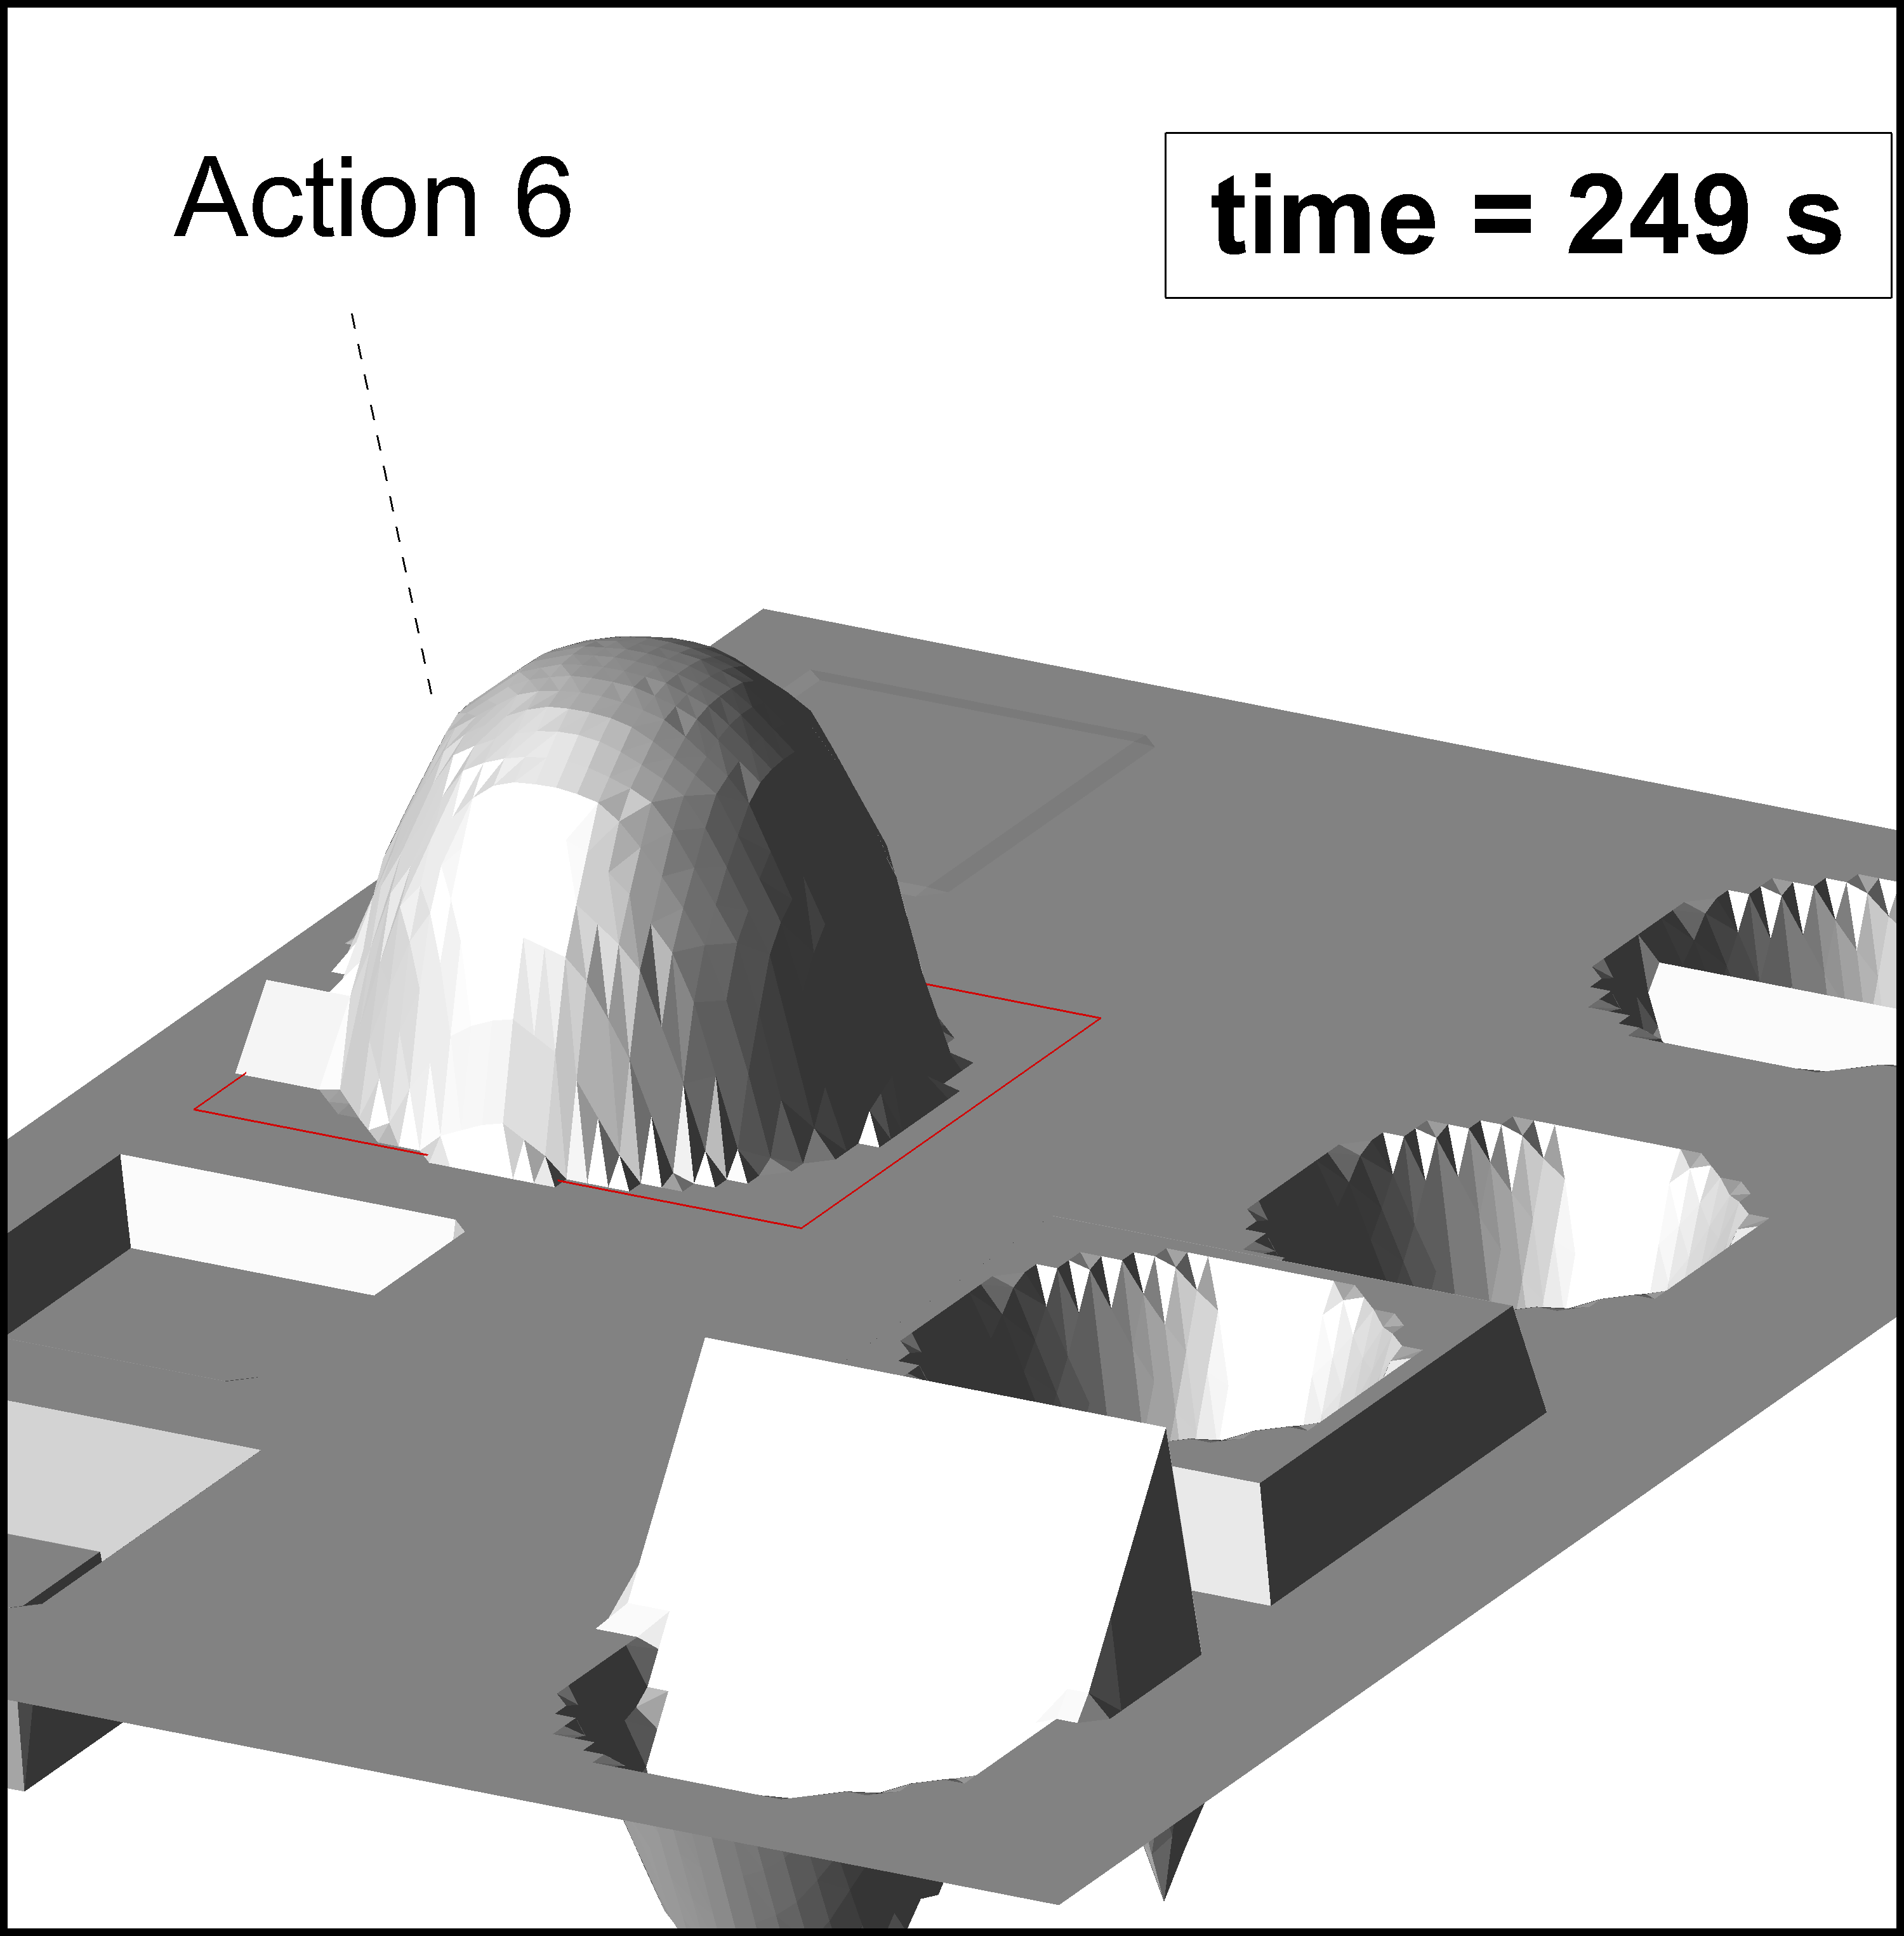
\includegraphics[width=0.45\textwidth]{img/Bild_Act6_249s.png}}
  \caption{Changes of the bottom while executing Action-5}
  \label{Act6}
\end{figure}

\newpage
Excerpt from the action file where the Action-6 is defined:
\\ \hspace*{3mm} \texttt{\small{/================================================================}}
\\ \hspace*{3mm} \texttt{\small{ACTION}}
\\ \hspace*{3mm} \texttt{\small{~~ActionType~~~~~~=~Backfill\_to\_level}}
\\ \hspace*{3mm} \texttt{\small{~~ReferenceLevel~~=~~GRID}}
\\ \hspace*{3mm} \texttt{\small{~~TimeStart~~~~~~~=~~2000.01.01-00:02:52~~/~[yyyy.mm.dd-hh:mm:ss]}}
\\ \hspace*{3mm} \texttt{\small{~~TimeEnd ~~~~~~~~=~~2000.01.01-00:04:22~~/~[yyyy.mm.dd-hh:mm:ss]}}
\\ \hspace*{3mm}
\\ \hspace*{3mm} \texttt{\small{~~FieldDump~~~~~~~=~~532\_ri\_middle\_low\_2}}
\\ \hspace*{3mm} \texttt{\small{~~CritDepth~~~~~~~=~~10.00~~~~~~~~~~~~~~~~/~[m]}}
\\ \hspace*{3mm} \texttt{\small{~~GrainClass~~~~~~=~~~1.00}}
\\ \hspace*{3mm} \texttt{\small{ENDACTION}}
\\ \hspace*{3mm} \texttt{\small{/================================================================}}




%      100 m$^3$ material will be dredged in the polygon named \texttt{201\_Abschnitt\_1\_2\_1000m**2}  defined in \texttt{\_DigPolys.dat} over a time period of 100 s.
%      The name must start with an integert number between 100 and 999. From position 4 is free text to help the user.
%      Only the number is the identifyer of the polygon. This Dredging area is located between 100,5 and 300,5 m of the flume with an area of 200 x 5 = 1000 m$^2$. In this part only
%      coarse material (dm=2mm) exists.
%      The dredging starts 50 s after the simulation start (2000.01.01-00:00:50) and ended 100 s later
%      (2000.01.01-00:02:30). This is defined in \texttt{\_DigActions.dat}.
%      The dredged material will create a final erosion of 0,1 m in the dredging area.
%      The dredging rate (calculeted by Nestor) is the dredging volume devided by the dredging time and the dredging area
%      $\frac{100 m^3/s}{100 s*1000 m^2}=0,001$ m/s
%
%      At the time when the dredging starts the dredged material will
%      be dumped in the polygon named \texttt{field 202\_Abschnitt\_6\_7\_1000m**2}, which is located between 700,5 and 900,5 m of the flume
%      with an area of 200 x 5 = 1000 m$^2$. The final sedimentation will be 0,1 m in the dumping field.
%      In this part originally only fine material is located (dm=0,1mm).
%      Due to a small dumping rate (preset to 0,0005 m/s), which is two times smaller than the dredging rate it takes 200 s to dump the material.
%
%      The sediment distribution will not be changed in the dredging area. In the
%      dumping area the mean grain size will be increased during the dumping of coarse material.
%      The final mean grain size is only 1,3 mm due to mixing processes of the Hirano layer model.
%      Without mixing processes, the active layer would completely consists of the coarse material and would have
%      a mean grain size of 2 mm as the sedimentation depth is as big as the active layer.
%
%      % - Reference:
%      %     This part gives the reference solution we are comparing to and
%      %     explicits the analytical solution when available;
%      %
%      %
%      \section{Reference}
%      %
%
%      % - Physical parameters:
%      %     This part specifies the geometry, details all the physical parameters
%      %     used to describe both porous media (soil model in particularly) and
%      %     solute characteristics (dispersion/diffusion coefficients, soil <=> pollutant interactions...)
%      %
%      %
%      \section{Physical parameters}
%      %
%      The simulation has set up with three grain classes (d=0,1 / 0,2 / 2 mm), but only the fine and the coarse material
%      are used. The bottom is discretised with three layers. A constant active layer (10 cm), an underlying stratum (10 cm)
%      and a last layer up to the rigid bed (9.8m).
%
%      The Meyer-Peter Mueller transport formula is used but the MPM parameter is set to zero which avoids sediment transport.
%      All bottom changes come from the dredging and dumping processes.
%      % - Geometry and Mesh:
%      %     This part describes the mesh used in the computation
%      %
%      %
%      \section{Geometry and Mesh}
%      %
%      A 1000 m long flume with three widening parts has been chosen as test geometry (figure \ref{ini}).
%      The width of the flume is 10 m and increases up to 30 m in the widening parts.
%      Two of the widening parts are 100 m long and the third is 200 m long.
%      The initial bottom has a continuous slope of 0,09 %.
%      The node area for every node is 1 m$^2$ in order to calculate dredging and dumping volumes very easily.
%
%      \begin{figure} [!ht]
%      \centering
%      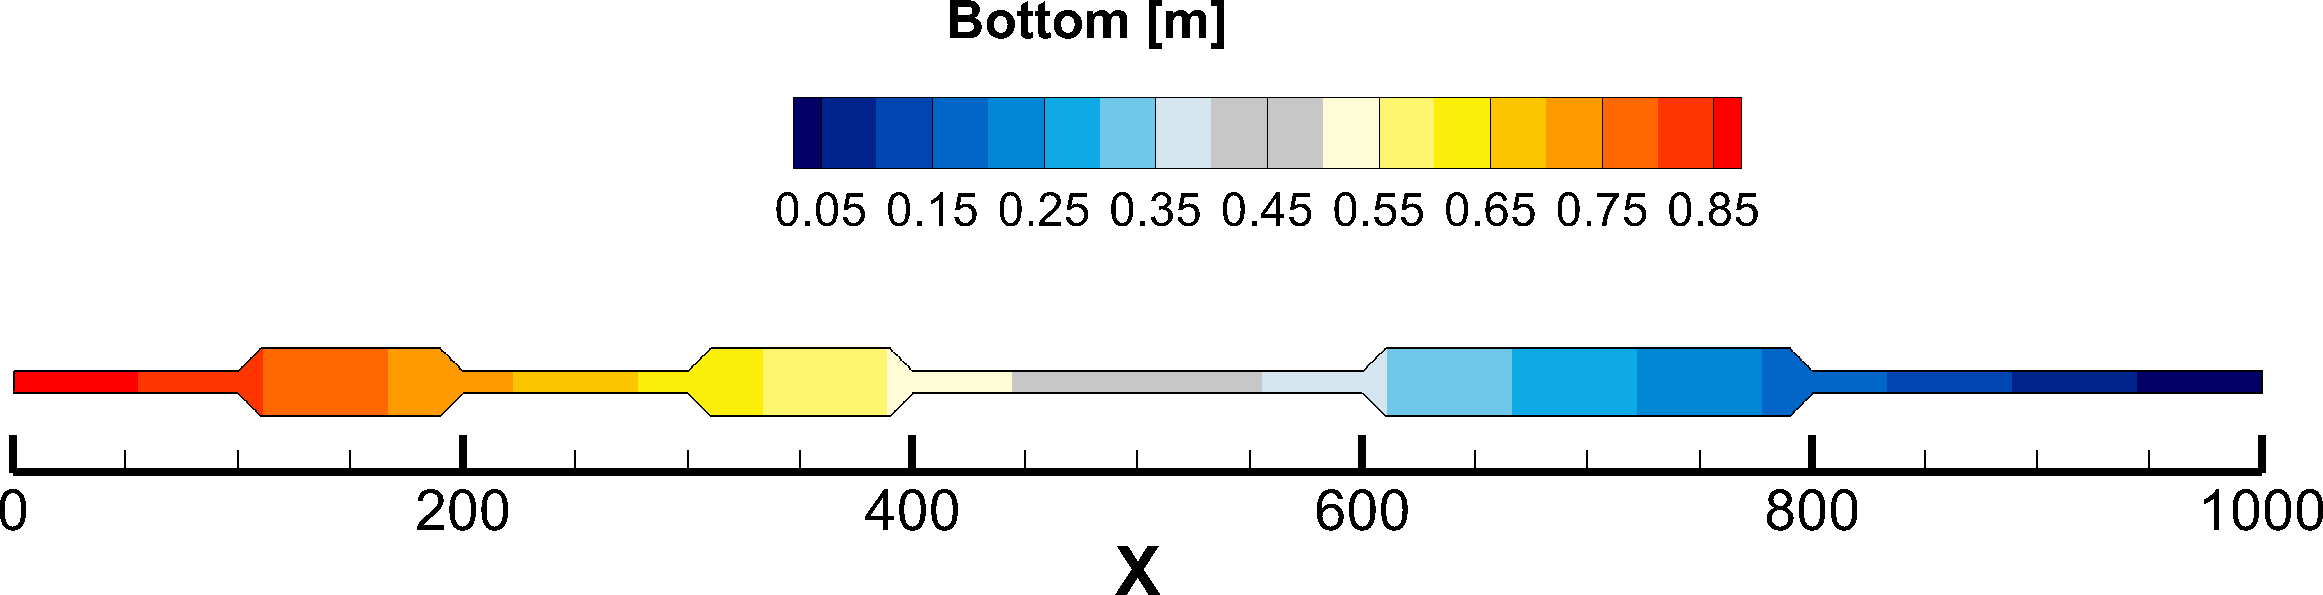
\includegraphics[scale=0.15]{img/ini_bottom.png}
%      \caption{Geometry of the test flume with three widening parts}\label{ini}
%      \end{figure}
%      The mesh consists of 18411 nodes and 34800 elements.
%
%      % - Initial and boundary conditions:
%      %     This part details both initial and boundary conditions used to simulate the case
%      %
%      %
%      \section{Initial and Boundary Conditions}
%      %
%      Steady state boundary conditions:
%      \begin{itemize}
%      \item{ Discharge at the inlet = 20 m$^3$/s}
%      \item Water depth at outlet = 1 m
%      \item Sedimentological equilibrium at the inlet (zF is constant, QS will be calculated)
%      \end{itemize}
%      Fully developed flow from a previous simulation is used as initial conditions.
%
%      With a time step of 1 s a simulation period of 250 s are computed.
%      % - Numerical parameters:
%      %     This part is used to specify the numerical parameters used
%      %     (adaptive time step, mass-lumping when necessary...)
%      %
%      %
%      \section{Numerical parameters}
%      %
%      % - Results:
%      %     We comment in this part the numerical results against the reference ones,
%      %     giving understanding keys and making assumptions when necessary.
%      %
%      %
%      \section{Results}
%      %
%      Figure \ref{result50} shows the evolution after 50 s (start of dredging and dumping),
%      after 100 s (end of dredging) and after 250 s (final simulation state and end of dumping process).
%
%      % Here is an example of how to include the graph generated by validateTELEMAC.py
%      % They should be in test_case/img
%      \begin{figure} [!ht]
%      \centering
%      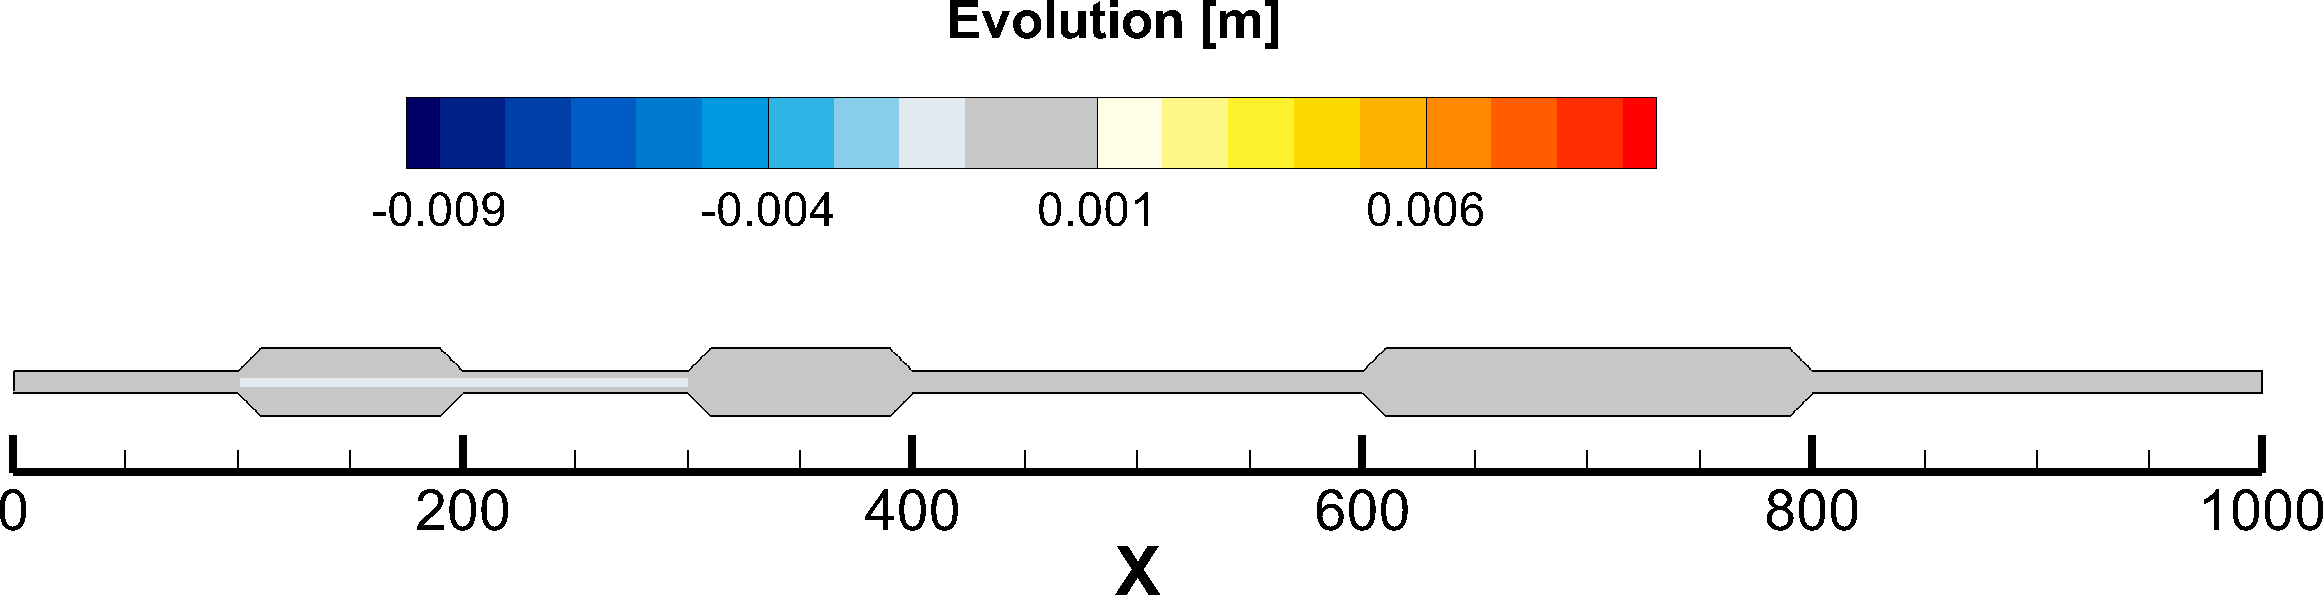
\includegraphics[scale=0.15]{img/result50.png}
%      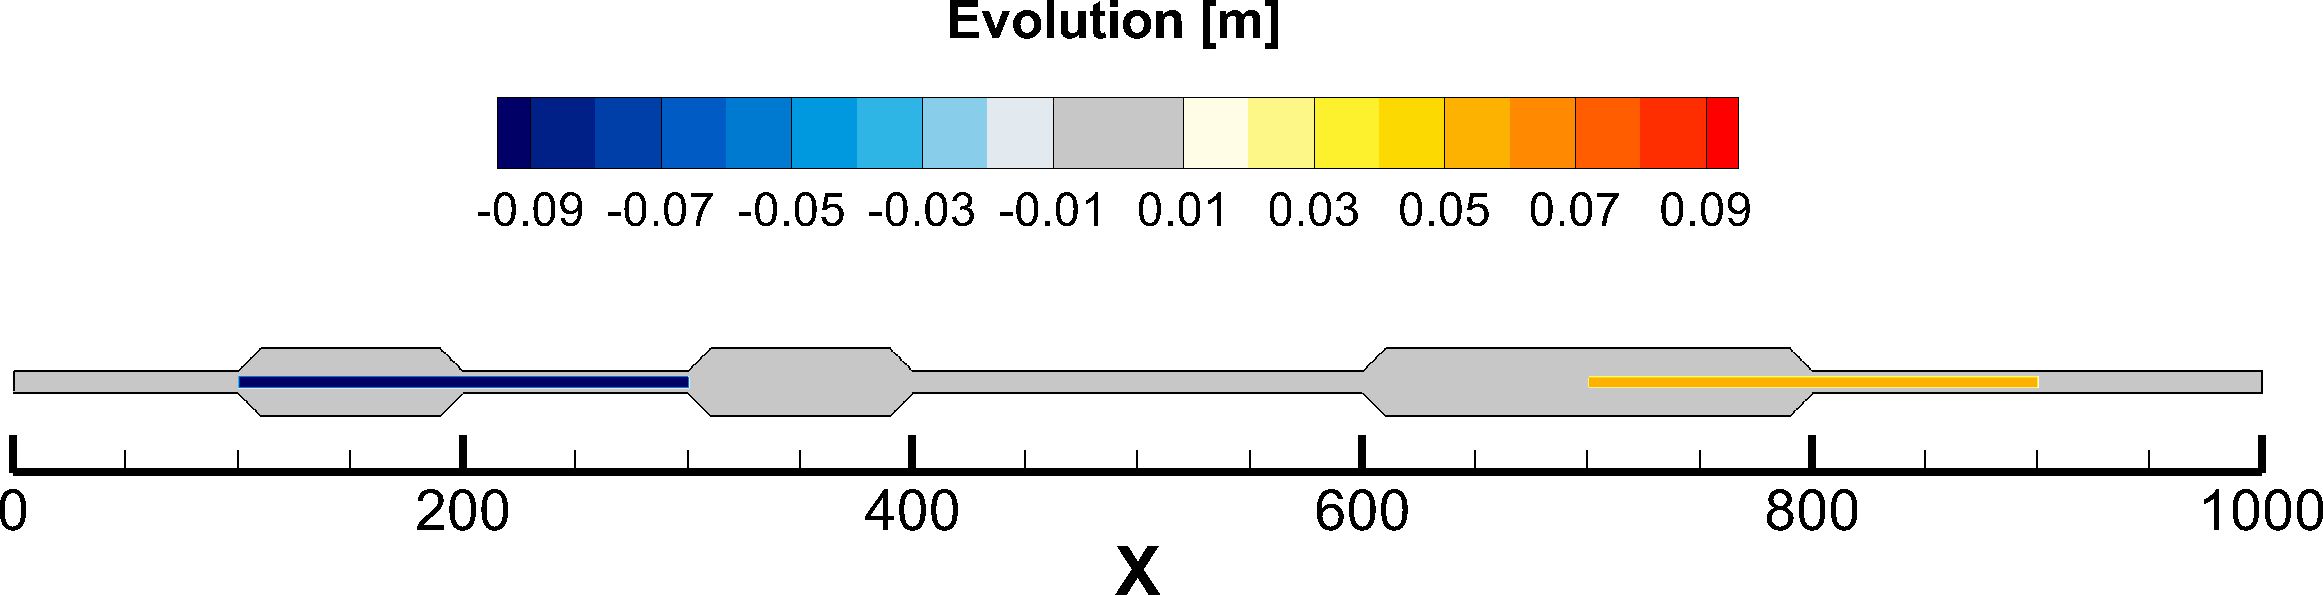
\includegraphics[scale=0.15]{img/result150.png}
%      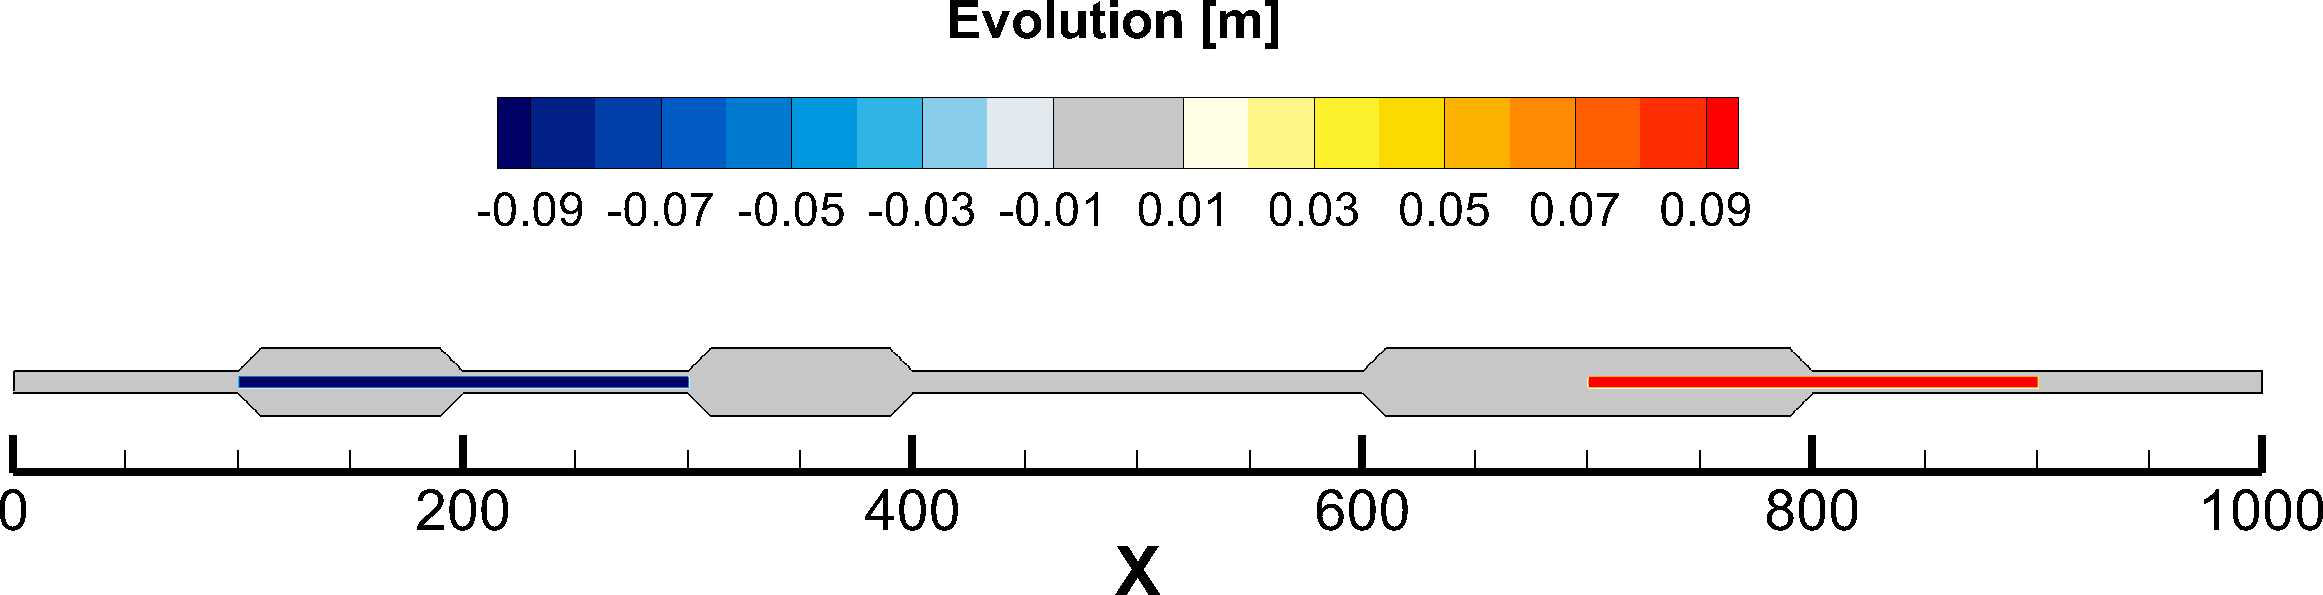
\includegraphics[scale=0.15]{img/result250.png}
%      \caption{Simulated evolution after 50, 100 and 250 s.}\label{result50}
%      \end{figure}
